% docs/sem_report/report.tex: semester project report (Study Oriented Project).
% Every number is \R{key}; keys are defined in macros.tex, generated by
%   python3 -I tools/make_paper_macros.py --target report
% from committed results files, and checked by
%   python3 -I tools/paper_numbers_check.py --macros docs/sem_report
% Build: make (repository copy, ID omitted) or make submission (copy with the student ID from the gitignored
% file student_id.local). See the Makefile.
\documentclass[11pt,a4paper]{report}
\usepackage[T1]{fontenc}
\usepackage{mathptmx}
\usepackage[margin=2.1cm]{geometry}
\usepackage{graphicx}
\usepackage{booktabs}
\usepackage{array}
\usepackage{tabularx}
\usepackage{longtable}

\usepackage{xcolor}
\usepackage{enumitem}
\usepackage{url}
\usepackage{tikz}
\usetikzlibrary{positioning,arrows.meta,fit,calc}
\usepackage[font=small,labelfont=bf]{caption}
\usepackage[hidelinks]{hyperref}
\usepackage[final]{microtype}
\usepackage{titlesec}
\titleformat{\chapter}[hang]{\LARGE\bfseries}{\thechapter}{0.8em}{}
\titlespacing*{\chapter}{0pt}{0pt}{14pt}
\setlength{\textfloatsep}{10pt plus 2pt minus 2pt}
\setlength{\floatsep}{8pt plus 2pt minus 2pt}
\setlength{\intextsep}{8pt plus 2pt minus 2pt}
\graphicspath{{figs/}{../../paper/v2/figs/}}
\setlength{\emergencystretch}{2em}
\makeatletter\g@addto@macro\UrlBreaks{\do-}\makeatother
\setlist{itemsep=2pt,topsep=4pt}
\makeatletter
\newcommand{\defnum}[2]{\expandafter\def\csname pn@#1\endcsname{#2}}
\DeclareRobustCommand{\R}[1]{\ifcsname pn@#1\endcsname\csname pn@#1\endcsname\else
  \PackageError{report}{number key '#1' is not defined in macros.tex}{Run tools/make_paper_macros.py --target report}\fi}
\makeatother
\newcommand{\umsq}{\textmu m\textsuperscript{2}}
\newcommand{\withdrawn}[1]{#1}
\newcommand{\reportdate}{November 2026}
\newcommand{\coursecode}{\fbox{\textsf{to be filled in}}}
\ifdefined\withid
  \input{student_id.local}
\else
  \newcommand{\studentid}{\textit{[omitted from the repository copy]}}
\fi
\newcolumntype{L}{>{\raggedright\arraybackslash}X}
% Generated by tools/make_paper_macros.py from committed results files. Do not edit by hand.
% Each line: \defnum{key}{shown}% format: source file:line [row | column] = full source value
\defnum{ds.rows}{45,840,617}% raw: results/P7/TABLES.md:8 /Rows in the file: ([\d,]+)/ group 1 = 45,840,617
\defnum{ds.tables}{26}% raw: results/P7/TABLES.md:8 /; (\d+) categorical columns = \d+ tables/ group 1 = 26
\defnum{ds.r2M}{2,000,000}% raw: results/P7/TABLES.md:8 /use the first ([\d,]+) and/ group 1 = 2,000,000
\defnum{ds.r10M}{10,000,000}% raw: results/P7/TABLES.md:8 /and the first ([\d,]+) of them/ group 1 = 10,000,000
\defnum{lab.2M}{2M}% raw: results/P9/SUMMARY.md:14 /\| (2M), 256 \|/ group 1 = 2M
\defnum{lab.10M}{10M}% raw: results/P9/SUMMARY.md:18 /\| (10M), 256 \|/ group 1 = 10M
\defnum{sz.16}{16}% raw: results/P11/PARTA.md:7 [2,000,000, 16 | entries] = 16
\defnum{sz.64}{64}% raw: results/P11/PARTA.md:8 [2,000,000, 64 | entries] = 64
\defnum{sz.256}{256}% raw: results/P11/PARTA.md:9 [2,000,000, 256 | entries] = 256
\defnum{sz.1000}{1,000}% raw: results/P7/TABLES.md:196 [1,000 | capacity (vectors, total)] = 1,000
\defnum{sz.10000}{10,000}% raw: results/P7/TABLES.md:197 [10,000 | capacity (vectors, total)] = 10,000
\defnum{sz.100000}{100,000}% raw: results/P7/TABLES.md:198 [100,000 | capacity (vectors, total)] = 100,000
\defnum{sz.p3min}{64}% raw: results/P7/TABLES.md:18 [64 | capacity (vectors per table)] = 64
\defnum{p11.acc.2M}{46,128,690}% raw: results/P11/PARTA.md:9 [2,000,000, 256 | accesses] = 46,128,690
\defnum{p11.acc.10M}{231,492,097}% raw: results/P11/PARTA.md:12 [10,000,000, 256 | accesses] = 231,492,097
\defnum{p3.window}{1}% raw: results/P7/TABLES.md:16 /W-TinyLFU \(Count-Min, window=(\d+)%\)/ group 1 = 1
\defnum{rtl.vecw}{128}% raw: results/P7/TABLES.md:464 [RTL parameter VECTOR_WIDTH (default) | value] = 128
\defnum{rtl.addrw}{20}% raw: results/P7/TABLES.md:463 [RTL parameter ADDR_WIDTH (default) | value] = 20
\defnum{rtl.cntw}{6}% raw: results/P7/TABLES.md:465 [RTL parameter COUNTER_WIDTH (default) | value] = 6
\defnum{rtl.groups}{16}% raw: results/P7/TABLES.md:466 [RTL parameter GROUPS (default) | value] = 16
\defnum{rtl.sat}{63}% raw: results/P7/TABLES.md:468 [RTL counter saturation value, 2^COUNTER_WIDTH - 1 | value] = 63
\defnum{rtl.tests}{7}% raw: results/P7/TABLES.md:469 [unit testbench tests | value] = 7
\defnum{rtl.simcap}{255}% raw: results/P7/TABLES.md:470 [trace simulator LFU counter cap (`min(N, ...)` in trace_sim/run_trace_sim.py) | value] = 255
\defnum{p10.kw}{8}% raw: results/P10/SUMMARY.md:4 /KW = EW\+1 = (\d+) bits/ group 1 = 8
\defnum{p11.ff.256}{8}% raw: results/P11/SUMMARY.md:24 /ptr width \(\+(\d+) / \+(\d+) / \+(\d+)\)/ group 3 = 8
\defnum{tool.yosys}{0.33}% raw: results/P7/TABLES.md:675 [Yosys | value] = 0.33
\defnum{tool.opensta}{3.1.0}% raw: results/P7/TABLES.md:673 /OpenSTA commit / version \| \w+ / ([\d.]+)/ group 1 = 3.1.0
\defnum{p9.runs}{24}% raw: results/P7/TABLES.md:944 /Runs with zero mismatches in both models: (\d+) of \d+/ group 1 = 24
\defnum{p9.req}{2,560,448}% raw: results/P7/TABLES.md:944 /requests compared: ([\d,]+)/ group 1 = 2,560,448
\defnum{p9.mism}{0}% raw: results/P7/TABLES.md:939 [256, 0, row0, full | mismatches (RTL-exact / structural)] = 0; same value in 48 more cells
\defnum{p9.slicereq}{200,000}% raw: results/P7/TABLES.md:939 [256, 0, row0, full | requests] = 200,000
\defnum{p14.B.64}{64}% raw: results/P14/SUMMARY.md:9 [64, per_table | B] = 64
\defnum{p14.pt.64}{74.35}% hit: results/P14/SUMMARY.md:9 [64, per_table | L2 read hit %] = 74.3535
\defnum{p14.cc.64}{76.35}% hit: results/P14/SUMMARY.md:10 [64, concat | L2 read hit %] = 76.3465
\defnum{p14.B.1024}{1,024}% raw: results/P14/SUMMARY.md:11 [1,024, per_table | B] = 1,024
\defnum{p14.pt.1024}{68.24}% hit: results/P14/SUMMARY.md:11 [1,024, per_table | L2 read hit %] = 68.2354
\defnum{p14.cc.1024}{67.45}% hit: results/P14/SUMMARY.md:12 [1,024, concat | L2 read hit %] = 67.4503
\defnum{p14.B.16384}{16,384}% raw: results/P14/SUMMARY.md:13 [16,384, per_table | B] = 16,384
\defnum{p14.pt.16384}{56.26}% hit: results/P14/SUMMARY.md:13 [16,384, per_table | L2 read hit %] = 56.2621
\defnum{p14.cc.16384}{54.04}% hit: results/P14/SUMMARY.md:14 [16,384, concat | L2 read hit %] = 54.0394
\defnum{p14.rows}{2M}% raw: results/P14/SUMMARY.md:1 /first (2M) rows/ group 1 = 2M
\defnum{p14.batches}{20}% raw: results/P14/SUMMARY.md:5 /Profiled: (\d+) batches/ group 1 = 20
\defnum{p14.dim}{128}% raw: results/P14/SUMMARY.md:4 /dim (\d+) float32/ group 1 = 128
\defnum{p14.cap}{100,000}% raw: results/P14/SUMMARY.md:22 /closest P3b capacity: ([\d,]+)/ group 1 = 100,000
\defnum{p14.vecbytes}{512}% raw: results/P14/SUMMARY.md:19 /A vector is (\d+) B/ group 1 = 512
\defnum{p3b.2M.256.LRU}{41.40}% hit: results/P7/TABLES.md:195 [256 | LRU] = 41.4010
\defnum{p3b.2M.1000.LRU}{53.68}% hit: results/P7/TABLES.md:196 [1,000 | LRU] = 53.6803
\defnum{p3b.2M.100000.LRU}{90.42}% hit: results/P7/TABLES.md:198 [100,000 | LRU] = 90.4240
\defnum{p3b.2M.256.LFUr}{47.67}% hit: results/P7/TABLES.md:195 [256 | LFU (gem5 LFURP — reset on eviction)] = 47.6719
\defnum{p3b.2M.1000.LFUr}{58.45}% hit: results/P7/TABLES.md:196 [1,000 | LFU (gem5 LFURP — reset on eviction)] = 58.4477
\defnum{p3b.2M.100000.LFUr}{91.61}% hit: results/P7/TABLES.md:198 [100,000 | LFU (gem5 LFURP — reset on eviction)] = 91.6117
\defnum{p3b.2M.256.LFUp}{41.00}% hit: results/P7/TABLES.md:195 [256 | LFU (persistent counters)] = 41.0006
\defnum{p3b.2M.1000.LFUp}{56.11}% hit: results/P7/TABLES.md:196 [1,000 | LFU (persistent counters)] = 56.1060
\defnum{p3b.2M.100000.LFUp}{92.58}% hit: results/P7/TABLES.md:198 [100,000 | LFU (persistent counters)] = 92.5839
\defnum{p3b.2M.256.WTLFU}{50.97}% hit: results/P7/TABLES.md:195 [256 | W-TinyLFU (Count-Min, window=1%)] = 50.9749
\defnum{p3b.2M.1000.WTLFU}{62.03}% hit: results/P7/TABLES.md:196 [1,000 | W-TinyLFU (Count-Min, window=1%)] = 62.0342
\defnum{p3b.2M.100000.WTLFU}{91.95}% hit: results/P7/TABLES.md:198 [100,000 | W-TinyLFU (Count-Min, window=1%)] = 91.9523
\defnum{p3b.2M.256.ARC}{50.92}% hit: results/P7/TABLES.md:195 [256 | ARC] = 50.9225
\defnum{p3b.2M.1000.ARC}{61.79}% hit: results/P7/TABLES.md:196 [1,000 | ARC] = 61.7905
\defnum{p3b.2M.100000.ARC}{92.37}% hit: results/P7/TABLES.md:198 [100,000 | ARC] = 92.3695
\defnum{p3.10M.256.LRU}{67.08}% hit: results/P7/TABLES.md:37 [256 | LRU] = 67.0796
\defnum{p3.10M.256.LFUr}{70.33}% hit: results/P7/TABLES.md:37 [256 | LFU (gem5 LFURP — reset on eviction)] = 70.3276
\defnum{p3.10M.256.LFUp}{68.33}% hit: results/P7/TABLES.md:37 [256 | LFU (persistent counters)] = 68.3280
\defnum{p3.10M.256.TLFU}{64.53}% hit: results/P7/TABLES.md:37 [256 | TinyLFU-exact (window=1%)] = 64.5267
\defnum{p3.10M.256.WTLFU}{73.10}% hit: results/P7/TABLES.md:37 [256 | W-TinyLFU (Count-Min, window=1%)] = 73.1009
\defnum{p3.10M.256.ARC}{72.42}% hit: results/P7/TABLES.md:37 [256 | ARC] = 72.4225
\defnum{p3.10M.256.BEL}{78.42}% hit: results/P7/TABLES.md:37 [256 | Belady (MIN, offline)] = 78.4180
\defnum{p3b.10M.256.LRU}{41.26}% hit: results/P7/TABLES.md:205 [256 | LRU] = 41.2640
\defnum{p3b.10M.1000.LRU}{53.47}% hit: results/P7/TABLES.md:206 [1,000 | LRU] = 53.4740
\defnum{p3b.10M.100000.LRU}{90.02}% hit: results/P7/TABLES.md:208 [100,000 | LRU] = 90.0219
\defnum{p3b.10M.256.LFUr}{48.16}% hit: results/P7/TABLES.md:205 [256 | LFU (gem5 LFURP — reset on eviction)] = 48.1592
\defnum{p3b.10M.1000.LFUr}{59.10}% hit: results/P7/TABLES.md:206 [1,000 | LFU (gem5 LFURP — reset on eviction)] = 59.1030
\defnum{p3b.10M.100000.LFUr}{90.93}% hit: results/P7/TABLES.md:208 [100,000 | LFU (gem5 LFURP — reset on eviction)] = 90.9315
\defnum{p3b.10M.256.LFUp}{38.49}% hit: results/P7/TABLES.md:205 [256 | LFU (persistent counters)] = 38.4896
\defnum{p3b.10M.1000.LFUp}{52.91}% hit: results/P7/TABLES.md:206 [1,000 | LFU (persistent counters)] = 52.9099
\defnum{p3b.10M.100000.LFUp}{92.39}% hit: results/P7/TABLES.md:208 [100,000 | LFU (persistent counters)] = 92.3924
\defnum{p3b.10M.256.WTLFU}{50.91}% hit: results/P7/TABLES.md:205 [256 | W-TinyLFU (Count-Min, window=1%)] = 50.9101
\defnum{p3b.10M.1000.WTLFU}{61.92}% hit: results/P7/TABLES.md:206 [1,000 | W-TinyLFU (Count-Min, window=1%)] = 61.9160
\defnum{p3b.10M.100000.WTLFU}{91.96}% hit: results/P7/TABLES.md:208 [100,000 | W-TinyLFU (Count-Min, window=1%)] = 91.9623
\defnum{p3b.10M.256.ARC}{50.88}% hit: results/P7/TABLES.md:205 [256 | ARC] = 50.8773
\defnum{p3b.10M.1000.ARC}{61.68}% hit: results/P7/TABLES.md:206 [1,000 | ARC] = 61.6774
\defnum{p3b.10M.100000.ARC}{92.18}% hit: results/P7/TABLES.md:208 [100,000 | ARC] = 92.1847
\defnum{p3b.drop.lo}{2.5109}% abs: results/P3b/SUMMARY.md:28 /\((-[\d.]+) to (-[\d.]+) pp/ group 1 = -2.5109
\defnum{p3b.drop.hi}{3.6112}% abs: results/P3b/SUMMARY.md:28 /\((-[\d.]+) to (-[\d.]+) pp/ group 2 = -3.6112
\defnum{p9.10M.256.v2}{39.82}% hit: results/P7/TABLES.md:1052 [256 | RTL-exact mode 0] = 39.8162
\defnum{p11.10M.256.v3}{48.16}% hit: results/P7/TABLES.md:1120 [256 | Rotate-victim m0 (v3 rule)] = 48.1592
\defnum{d.v3lru}{6.90}% sub (results/P7/TABLES.md:1120 [256 | Rotate-victim m0 (v3 rule)] = 48.1592) - (results/P7/TABLES.md:1052 [256 | LRU] = 41.2640), 2 decimals
\defnum{d.v3v2}{8.34}% sub (results/P7/TABLES.md:1120 [256 | Rotate-victim m0 (v3 rule)] = 48.1592) - (results/P7/TABLES.md:1052 [256 | RTL-exact mode 0] = 39.8162), 2 decimals
\defnum{p9.prev.v2}{118,522}% raw: results/P7/TABLES.md:983 [row0, 256 | RTL-exact mode 0] = 118,522
\defnum{p9.prev.v2.n}{118,523}% raw: results/P7/TABLES.md:983 [row0, 256 | RTL-exact mode 0] = 118,523
\defnum{p9.prev.old}{0}% raw: results/P7/TABLES.md:983 [row0, 256 | LFU-reset (oldest)] = 0
\defnum{p9.prev.old.n}{96,362}% raw: results/P7/TABLES.md:983 [row0, 256 | LFU-reset (oldest)] = 96,362
\defnum{p9.sat}{0}% raw: results/P7/TABLES.md:1027 [256 | sat] = 0; same value in 8 more cells
\defnum{p9.int}{0}% raw: results/P7/TABLES.md:1027 [256 | interaction] = 0; same value in 8 more cells
\defnum{p9.rec}{100.0}% raw: results/P7/TABLES.md:1039 [256 | recovered % Rotate-victim mode 0] = 100.0; same value in 8 more cells
\defnum{p11.tl.16}{10}% raw: results/P11/PARTA.md:7 [2,000,000, 16 | tables with v3 < v2 (of 26)] = 10; same value in 1 more cells
\defnum{p11.tl.256}{2}% raw: results/P11/PARTA.md:9 [2,000,000, 256 | tables with v3 < v2 (of 26)] = 2; same value in 1 more cells
\defnum{p10.16.row0.v3}{17,035}% raw: results/P7/TABLES.md:1089 [16, 0, row0 | RTL hits] = 17,035
\defnum{p10.16.row0.v2}{19,946}% raw: results/P7/TABLES.md:1089 [16, 0, row0 | v2-rule hits (m0) / equals P9 v2 log (m1)] = 19,946
\defnum{p10.16.row1M.v3}{5,217}% raw: results/P7/TABLES.md:1090 [16, 0, row1M | RTL hits] = 5,217
\defnum{p10.16.row1M.v2}{18,254}% raw: results/P7/TABLES.md:1090 [16, 0, row1M | v2-rule hits (m0) / equals P9 v2 log (m1)] = 18,254
\defnum{p10.256.row0.v3}{103,382}% raw: results/P7/TABLES.md:1093 [256, 0, row0 | RTL hits] = 103,382
\defnum{p10.256.row0.v2}{81,221}% raw: results/P7/TABLES.md:1093 [256, 0, row0 | v2-rule hits (m0) / equals P9 v2 log (m1)] = 81,221
\defnum{p10.runs}{12}% raw: results/P10/SUMMARY.md:14 /Mismatches = 0 in all (\d+) runs/ group 1 = 12
\defnum{p10.mism}{0}% raw: results/P10/SUMMARY.md:14 /Mismatches = (\d+) in all \d+ runs/ group 1 = 0
\defnum{p10.mut}{3}% raw: results/P10/SUMMARY.md:12 /all (\d+) caught/ group 1 = 3
\defnum{p11.mut.tb}{140}% raw: results/P11/SUMMARY.md:36 /(\d+) were killed by the testbench/ group 1 = 140
\defnum{p11.mut.ls}{5}% raw: results/P11/SUMMARY.md:36 /, (\d+) by lockstep against/ group 1 = 5
\defnum{p11.eq.16}{3,520}% raw: results/P11/SUMMARY.md:26 /Also proven at depth 16: ([\d,]+) of/ group 1 = 3,520
\defnum{p11.eq.64}{12,578}% raw: results/P11/SUMMARY.md:26 /all ([\d,]+) \$equiv cells proven/ group 1 = 12,578
\defnum{p11.gls.n}{24}% raw: results/P11/SUMMARY.md:34 /- (\d+)/\d+ pass: all/ group 1 = 24
\defnum{p11.gls.mism}{0}% raw: results/P11/SUMMARY.md:31 /\| (0) in every task \|/ group 1 = 0
\defnum{p13.mism}{0}% raw: results/P13/TABLES.md:11 [v3, row0 | SDF: mismatching; X (netlist/RTL) cycles] = 0; same value in 8 more cells
\defnum{p15.mism}{0}% raw: results/P15/TABLES.md:175 [v3, row0, sdf | mismatching cycles] = 0; same value in 12 more cells
\defnum{p15.sdf.path}{100.00}% raw: results/P15/TABLES.md:175 [v3, row0, sdf | SDF path delays annotated] = 100.00; same value in 1 more cells
\defnum{p15.sdf.check}{0.00}% raw: results/P15/TABLES.md:175 [v3, row0, sdf | SDF timing checks annotated] = 0.00; same value in 1 more cells
\defnum{p11.nnoise}{6.44}% raw: results/P11/SUMMARY.md:23 /This ([\d.]+)% is the observed flow variation/ group 1 = 6.44
\defnum{p12.br.256.met}{0.8}% raw: results/P12/TABLES.md:131 [v2, 0, 256 | tightest met (ns)] = 0.8; same value in 4 more cells
\defnum{p12.br.256.fail}{0.65}% raw: results/P12/TABLES.md:131 [v2, 0, 256 | loosest failed (ns)] = 0.65; same value in 4 more cells
\defnum{p12.per.min}{0.5}% raw: results/P12/TABLES.md:129 [v2, 0, 16 | periods run (ns)] = 0.5
\defnum{p12.per.max}{2.0}% raw: results/P12/TABLES.md:129 [v2, 0, 16 | periods run (ns)] = 2.0
\defnum{p12.io}{0.2}% raw: results/P12/TABLES.md:3 /I/O delay ([\d.]+) x period/ group 1 = 0.2
\defnum{p12.relax}{2.0}% raw: results/P12/TABLES.md:92 [0, 16, 2.0 | period (ns)] = 2.0
\defnum{p12.mo.v2}{4.06}% abs: results/P12/TABLES.md:164 [v2, 0.65, merge-off | Fmax change] = +4.06
\defnum{p12.fmo.v2}{1310.6}% raw: results/P12/TABLES.md:164 [v2, 0.65, merge-off | Fmax (MHz)] = 1310.6
\defnum{p12.f.v2}{1259.4}% raw: results/P12/TABLES.md:163 [v2, 0.65, normal | Fmax (MHz)] = 1259.4
\defnum{p12.mo.v3}{4.60}% abs: results/P12/TABLES.md:168 [v3, 0.65, merge-off | Fmax change] = +4.60
\defnum{p12.fmo.v3}{1314.1}% raw: results/P12/TABLES.md:168 [v3, 0.65, merge-off | Fmax (MHz)] = 1314.1
\defnum{p12.f.v3}{1256.3}% raw: results/P12/TABLES.md:167 [v3, 0.65, normal | Fmax (MHz)] = 1256.3
\defnum{p12.copies}{320}% raw: results/P12/TABLES.md:164 [v2, 0.65, merge-off | req_addr_grp flops] = 320; same value in 4 more cells
\defnum{p13.period}{0.8}% raw: results/P13/SUMMARY.md:2 /clock ([\d.]+) ns;/ group 1 = 0.8
\defnum{p13.req}{200,000}% raw: results/P13/SUMMARY.md:2 /([\d,]+) requests per slice/ group 1 = 200,000
\defnum{p13.E.v2.row0}{743.94}% raw: results/P13/TABLES.md:28 [v2, row0 | energy per request] = 743.94
\defnum{p13.E.v2.row1M}{737.64}% raw: results/P13/TABLES.md:29 [v2, row1M | energy per request] = 737.64
\defnum{p13.E.v3.row0}{676.39}% raw: results/P13/TABLES.md:30 [v3, row0 | energy per request] = 676.39
\defnum{p13.E.v3.row1M}{682.79}% raw: results/P13/TABLES.md:31 [v3, row1M | energy per request] = 682.79
\defnum{p13.logic.hi}{2.21}% max of 4: results/P13/TABLES.md:28 [v2, row0 | logic share] = 1.49; results/P13/TABLES.md:29 [v2, row1M | logic share] = 1.49; results/P13/TABLES.md:30 [v3, row0 | logic share] = 2.00; results/P13/TABLES.md:31 [v3, row1M | logic share] = 2.21
\defnum{p15.met}{1.0}% raw: results/P15/TABLES.md:128 [v2_m0_d256_p0.8_nomerge, target-slack flow, latest hold pass at each period | tightest met ns] = 1.0; same value in 1 more cells
\defnum{p15.fail}{0.9}% raw: results/P15/TABLES.md:128 [v2_m0_d256_p0.8_nomerge, target-slack flow, latest hold pass at each period | loosest failed ns] = 0.9; same value in 1 more cells
\defnum{p15.oldfail}{1.1}% raw: results/P15/SUMMARY.md:18 /Earlier flows failed ([\d.]+)-([\d.]+) ns/ group 2 = 1.1
\defnum{p15.tslack}{0.03}% raw: results/P15/SUMMARY.md:8 /setup target slack ([\d.]+) ns/ group 1 = 0.03
\defnum{p15.tt.v}{1.00}% raw: results/P15/SUMMARY.md:2 /typical ([\d.]+) V (\d+) C/ group 1 = 1.00
\defnum{p15.tt.t}{25}% raw: results/P15/SUMMARY.md:2 /typical ([\d.]+) V (\d+) C/ group 2 = 25
\defnum{p15.core.v2}{379007.7}% raw: results/P15/TABLES.md:36 [v2_m0_d256_p0.8_nomerge, nodvtsh database + hold target slack 0.01, optDesign -postRoute -hold, ecoRoute -fix_drc (+1 if verify_drc found a violation), 1.0 | core area] = 379007.7
\defnum{p15.rs.v2}{8}% raw: results/P15/TABLES.md:104 [v2_m0_d256_p0.8_nomerge, 1.0 | resized to single-row] = 8
\defnum{p15.core.v3}{376946.3}% raw: results/P15/TABLES.md:51 [v3_m0_d256_p0.8_nomerge, nodvtsh database + hold target slack 0.01, optDesign -postRoute -hold, ecoRoute -fix_drc (+1 if verify_drc found a violation), 1.0 | core area] = 376946.3
\defnum{p15.rs.v3}{6}% raw: results/P15/TABLES.md:116 [v3_m0_d256_p0.8_nomerge, 1.0 | resized to single-row] = 6
\defnum{p15.wtv}{2}% raw: results/P15/TABLES.md:36 [v2_m0_d256_p0.8_nomerge, nodvtsh database + hold target slack 0.01, optDesign -postRoute -hold, ecoRoute -fix_drc (+1 if verify_drc found a violation), 1.0 | well-tap viol. full core] = 2; same value in 1 more cells
\defnum{p15.d16.period}{0.8}% raw: results/P15/TABLES.md:40 [v3_m0_d16_p0.8, multi-row dont_use, 0.8 | period ns] = 0.8
\defnum{p15.gls.period}{1.1}% raw: results/P15/TABLES.md:202 /## v3 against v2 per slice \(([\d.]+) ns/ group 1 = 1.1
\defnum{p15.E.v2.row0}{1011.49}% raw: results/P15/TABLES.md:197 [v2, row0 | energy per request] = 1011.49
\defnum{p15.E.v2.row1M}{1000.41}% raw: results/P15/TABLES.md:198 [v2, row1M | energy per request] = 1000.41
\defnum{p15.E.v3.row0}{924.68}% raw: results/P15/TABLES.md:199 [v3, row0 | energy per request] = 924.68
\defnum{p15.E.v3.row1M}{932.72}% raw: results/P15/TABLES.md:200 [v3, row1M | energy per request] = 932.72
\defnum{p15.logic.lo}{2.48}% min of 4: results/P15/TABLES.md:197 [v2, row0 | logic (combinational) share = uncertainty bound] = 2.72; results/P15/TABLES.md:198 [v2, row1M | logic (combinational) share = uncertainty bound] = 2.48; results/P15/TABLES.md:199 [v3, row0 | logic (combinational) share = uncertainty bound] = 3.21; results/P15/TABLES.md:200 [v3, row1M | logic (combinational) share = uncertainty bound] = 3.34
\defnum{p15.logic.hi}{3.34}% max of 4: results/P15/TABLES.md:197 [v2, row0 | logic (combinational) share = uncertainty bound] = 2.72; results/P15/TABLES.md:198 [v2, row1M | logic (combinational) share = uncertainty bound] = 2.48; results/P15/TABLES.md:199 [v3, row0 | logic (combinational) share = uncertainty bound] = 3.21; results/P15/TABLES.md:200 [v3, row1M | logic (combinational) share = uncertainty bound] = 3.34
\defnum{p15.cov.v2}{48.74}% raw: results/P15/TABLES.md:197 [v2, row0 | driver nets annotated] = 48.74; same value in 1 more cells
\defnum{p15.cov.v3}{48.95}% raw: results/P15/TABLES.md:199 [v3, row0 | driver nets annotated] = 48.95; same value in 1 more cells
\defnum{p15.dE.row0.abs}{8.58}% abs: results/P15/TABLES.md:205 [row0 | change] = -8.58
\defnum{p15.dE.row1M.abs}{6.77}% abs: results/P15/TABLES.md:206 [row1M | change] = -6.77
\defnum{p16.ss.v}{0.90}% raw: results/P16/SUMMARY.md:2 /ss = slow ([\d.]+) V (\d+) C/ group 1 = 0.90
\defnum{p16.ss.t}{125}% raw: results/P16/SUMMARY.md:2 /ss = slow ([\d.]+) V (\d+) C/ group 2 = 125
\defnum{p16.ff.v}{1.10}% raw: results/P16/SUMMARY.md:3 /ff = fast ([\d.]+) V (-\d+) C/ group 1 = 1.10
\defnum{p16.ff.t}{\ensuremath{-}40}% raw: results/P16/SUMMARY.md:3 /ff = fast ([\d.]+) V (-\d+) C/ group 2 = -40
\defnum{p16.dp.v2.10}{1.257}% raw: results/P16/TABLES.md:68 [d256 v2, 1.0 | derived slow-corner period ns] = 1.257
\defnum{p16.dp.v3.10}{1.236}% raw: results/P16/TABLES.md:69 [d256 v3, 1.0 | derived slow-corner period ns] = 1.236
\defnum{p16.io.indelay}{0.200}% raw: results/P16/TABLES.md:80 [ss | worst in2reg hold path: input delay] = 0.200
\defnum{p16.io.clk}{0.414}% raw: results/P16/TABLES.md:80 [ss | clock arrival at register] = 0.414
\defnum{p16.io.slack}{\ensuremath{-}0.212}% raw: results/P16/TABLES.md:80 [ss | slack] = -0.212
\defnum{p16.io.lat}{\ensuremath{-}0.315}% raw: results/P16/TABLES.md:79 [tt | capture clock source latency] = -0.315
\defnum{p16.io.tree}{0.319}% raw: results/P16/TABLES.md:79 [tt | tree insertion delay (arrival - source latency)] = 0.319
\defnum{p16.io.ttslack}{0.191}% raw: results/P16/TABLES.md:79 [tt | slack] = 0.191
\defnum{p9.ff.rs}{8}% raw: results/P9/CANDIDATES.md:12 [R2 Rotate-step | added state (by construction, depth 256, 16 groups)] = 8; same value in 1 more cells
\defnum{p9.ff.yb}{256}% raw: results/P9/CANDIDATES.md:13 [R3 Young-bit | added state (by construction, depth 256, 16 groups)] = 256
\defnum{p9.probe.n}{60}% raw: results/P7/TABLES.md:1000 /Synthetic probe \(not Criteo; (\d+) random Zipf traces.*Rotate-victim mode 0 (\d+), Rotate-step mode 0 (\d+)/ group 1 = 60
\defnum{p9.probe.rv}{9}% raw: results/P7/TABLES.md:1000 /Synthetic probe \(not Criteo; (\d+) random Zipf traces.*Rotate-victim mode 0 (\d+), Rotate-step mode 0 (\d+)/ group 2 = 9
\defnum{p9.probe.rs}{54}% raw: results/P7/TABLES.md:1000 /Synthetic probe \(not Criteo; (\d+) random Zipf traces.*Rotate-victim mode 0 (\d+), Rotate-step mode 0 (\d+)/ group 3 = 54
\defnum{p15.ladiff}{2.30}% ratio 100 x ((results/P15/TABLES.md:51 [v3_m0_d256_p0.8_nomerge, nodvtsh database + hold target slack 0.01, optDesign -postRoute -hold, ecoRoute -fix_drc (+1 if verify_drc found a violation), 1.0 | logic cell area] = 246532.5) / (results/P15/TABLES.md:36 [v2_m0_d256_p0.8_nomerge, nodvtsh database + hold target slack 0.01, optDesign -postRoute -hold, ecoRoute -fix_drc (+1 if verify_drc found a violation), 1.0 | logic cell area] = 240979.5) - 1), 2 decimals
\defnum{p12.noise}{3.41}% abs: results/P12/SUMMARY.md:32 /the same-logic mode-1 difference reaches (-[\d.]+)%/ group 1 = -3.41
\defnum{p14.l2mib}{50}% div (results/P14/SUMMARY.md:22 /H100 L2 = ([\d,]+) B/ group 1 = 52,428,800) / 1048576 (1 MiB = 1,048,576 bytes), exact
\defnum{p13.mW.v2.row0}{227.987}% mW: results/P13/TABLES.md:28 [v2, row0 | total] = 2.27987e-01
\defnum{p15.mW.v2.row0}{225.440}% mW: results/P15/TABLES.md:197 [v2, row0 | total] = 2.25440e-01
\defnum{p13.mW.v2.row1M}{227.986}% mW: results/P13/TABLES.md:29 [v2, row1M | total] = 2.27986e-01
\defnum{p15.mW.v2.row1M}{224.874}% mW: results/P15/TABLES.md:198 [v2, row1M | total] = 2.24874e-01
\defnum{p13.mW.v3.row0}{229.104}% mW: results/P13/TABLES.md:30 [v3, row0 | total] = 2.29104e-01
\defnum{p15.mW.v3.row0}{227.787}% mW: results/P15/TABLES.md:199 [v3, row0 | total] = 2.27787e-01
\defnum{p13.mW.v3.row1M}{229.615}% mW: results/P13/TABLES.md:31 [v3, row1M | total] = 2.29615e-01
\defnum{p15.mW.v3.row1M}{228.118}% mW: results/P15/TABLES.md:200 [v3, row1M | total] = 2.28118e-01
\defnum{p15.reg.v2.row0}{72.74}% raw: results/P15/TABLES.md:197 [v2, row0 | register share] = 72.74
\defnum{p15.clk.v2.row0}{24.54}% raw: results/P15/TABLES.md:197 [v2, row0 | clock (clock tree) share] = 24.54
\defnum{p15.logic.v2.row0}{2.72}% raw: results/P15/TABLES.md:197 [v2, row0 | logic (combinational) share = uncertainty bound] = 2.72
\defnum{p15.reg.v3.row0}{71.98}% raw: results/P15/TABLES.md:199 [v3, row0 | register share] = 71.98
\defnum{p15.clk.v3.row0}{24.80}% raw: results/P15/TABLES.md:199 [v3, row0 | clock (clock tree) share] = 24.80
\defnum{p15.logic.v3.row0}{3.21}% raw: results/P15/TABLES.md:199 [v3, row0 | logic (combinational) share = uncertainty bound] = 3.21
\defnum{p13.dE.row0.abs}{9.08}% abs: results/P13/TABLES.md:39 [row0 | change] = -9.08
\defnum{p13.dE.row1M.abs}{7.44}% abs: results/P13/TABLES.md:40 [row1M | change] = -7.44
\defnum{d.in2reg.other}{4}% sub (results/P16/TABLES.md:91 /Failing hold paths at ss in timeDesign: (\d+)/ group 1 = 6507) - (results/P16/TABLES.md:90 [ss | violating hold paths in2reg] = 6503), 0 decimals
\defnum{p13.fill.max}{3}% raw: results/P13/SUMMARY.md:29 /(\d)-(\d) random cycles/ group 2 = 3
\defnum{p9.rvdiff.hi.abs}{918}% abs: results/P9/SUMMARY.md:37 /Rotate-victim differs by (-?\d+) to (\+[\d,]+) hits/ group 2 = +918
\defnum{p12.a.16.m0.abs}{0.40}% abs: results/P12/TABLES.md:92 [0, 16, 2.0 | area change] = +0.40
\defnum{p12.mo.a.v3.abs}{4.06}% abs: results/P12/TABLES.md:168 [v3, 0.65, merge-off | area change] = +4.06
\defnum{p12.mo.a08.v3.abs}{1.10}% abs: results/P12/TABLES.md:170 [v3, 0.8, merge-off | area change] = +1.10
\defnum{p12.a.256.m1.abs}{0.65}% abs: results/P12/TABLES.md:122 [1, 256, 2.0 | area change] = -0.65
\defnum{p1.mutants}{6}% raw: results/P1/SUMMARY.md:25 /(\d+) mutants x (\d+) modes = (\d+) runs/ group 1 = 6
\defnum{p1.runs}{12}% raw: results/P1/SUMMARY.md:25 /(\d+) mutants x (\d+) modes = (\d+) runs/ group 3 = 12
\defnum{p1.survive}{3}% raw: results/P1/SUMMARY.md:29 /(\d+) runs survive as expected/ group 1 = 3
\defnum{p2.archive}{4576820670}% raw: results/P2/SUMMARY.md:7 /Archive size (\d+) bytes/ group 1 = 4576820670
\defnum{p2.train}{11147184845}% raw: results/P2/SUMMARY.md:13 [train.txt | Bytes] = 11147184845
\defnum{p2.cols}{40}% raw: results/P2/SUMMARY.md:19 /Rows without (\d+) tab-separated columns/ group 1 = 40
\defnum{p2.bad}{0}% raw: results/P2/SUMMARY.md:19 /Rows without \d+ tab-separated columns: (\d+)/ group 1 = 0
\defnum{p2.c.lo}{14}% raw: results/P2/SUMMARY.md:22 /Categorical columns (\d+)-(\d+):/ group 1 = 14
\defnum{p2.c.hi}{39}% raw: results/P2/SUMMARY.md:22 /Categorical columns (\d+)-(\d+):/ group 2 = 39
\defnum{p2.hexlen}{8}% raw: results/P2/SUMMARY.md:22 /fields are (\d+)-char lowercase hex/ group 1 = 8
\defnum{p2.hex}{1061312074}% raw: results/P2/SUMMARY.md:22 /: (\d+) fields are \d+-char lowercase hex/ group 1 = 1061312074
\defnum{p2.empty}{130543968}% raw: results/P2/SUMMARY.md:22 /hex, (\d+) empty/ group 1 = 130543968
\defnum{p2.fields}{1191856042}% raw: results/P2/SUMMARY.md:24 /= (\d+) = \d+ rows/ group 1 = 1191856042
\defnum{p3.t2M.p.win}{18}% raw: results/P3/SUMMARY.md:25 /2M: persistent LFU > LRU on (\d+) tables, tie on (\d+), worse on (\d+); LFURP > LRU on (\d+), tie (\d+), worse on (\d+)/ group 1 = 18
\defnum{p3.t2M.p.tie}{8}% raw: results/P3/SUMMARY.md:25 /2M: persistent LFU > LRU on (\d+) tables, tie on (\d+), worse on (\d+); LFURP > LRU on (\d+), tie (\d+), worse on (\d+)/ group 2 = 8
\defnum{p3.t2M.p.lose}{0}% raw: results/P3/SUMMARY.md:25 /2M: persistent LFU > LRU on (\d+) tables, tie on (\d+), worse on (\d+); LFURP > LRU on (\d+), tie (\d+), worse on (\d+)/ group 3 = 0
\defnum{p3.t2M.r.win}{17}% raw: results/P3/SUMMARY.md:25 /2M: persistent LFU > LRU on (\d+) tables, tie on (\d+), worse on (\d+); LFURP > LRU on (\d+), tie (\d+), worse on (\d+)/ group 4 = 17
\defnum{p3.t2M.r.tie}{8}% raw: results/P3/SUMMARY.md:25 /2M: persistent LFU > LRU on (\d+) tables, tie on (\d+), worse on (\d+); LFURP > LRU on (\d+), tie (\d+), worse on (\d+)/ group 5 = 8
\defnum{p3.t2M.r.lose}{1}% raw: results/P3/SUMMARY.md:25 /2M: persistent LFU > LRU on (\d+) tables, tie on (\d+), worse on (\d+); LFURP > LRU on (\d+), tie (\d+), worse on (\d+)/ group 6 = 1
\defnum{p3.t10M.p.lose}{6}% raw: results/P3/SUMMARY.md:26 /10M: persistent LFU > LRU on (\d+), tie (\d+), worse on (\d+)/ group 3 = 6
\defnum{p3.t10M.r.lose}{2}% raw: results/P3/SUMMARY.md:27 /LFURP > LRU on (\d+), tie (\d+), worse on (\d+) \(tables 1, 4\)/ group 3 = 2
\defnum{p3.zipf.n}{24}% raw: results/P3/SUMMARY.md:32 /(\d+) of (\d+) tables fitted at both sizes/ group 1 = 24
\defnum{p3.zipf.lo}{1.0759}% raw: results/P3/SUMMARY.md:33 /10M: ([\d.]+) \(table 2\) to ([\d.]+) \(table 5\)/ group 1 = 1.0759
\defnum{p3.zipf.hi}{5.6033}% raw: results/P3/SUMMARY.md:33 /10M: ([\d.]+) \(table 2\) to ([\d.]+) \(table 5\)/ group 2 = 5.6033
\defnum{p3.large.thr}{150,000}% raw: results/P7/TABLES.md:111 /unique ids >= ([\d,]+) at both row counts/ group 1 = 150,000
\defnum{p3b.2M.10000.LRU}{75.40}% hit: results/P7/TABLES.md:197 [10,000 | LRU] = 75.4015
\defnum{p3b.2M.10000.LFUr}{77.97}% hit: results/P7/TABLES.md:197 [10,000 | LFU (gem5 LFURP — reset on eviction)] = 77.9677
\defnum{p3b.2M.10000.LFUp}{81.93}% hit: results/P7/TABLES.md:197 [10,000 | LFU (persistent counters)] = 81.9279
\defnum{p3b.2M.10000.WTLFU}{80.86}% hit: results/P7/TABLES.md:197 [10,000 | W-TinyLFU (Count-Min, window=1%)] = 80.8618
\defnum{p3b.2M.10000.ARC}{80.76}% hit: results/P7/TABLES.md:197 [10,000 | ARC] = 80.7592
\defnum{p3.10M.64.LRU}{55.35}% hit: results/P7/TABLES.md:35 [64 | LRU] = 55.3528
\defnum{p3.10M.64.LFUr}{59.51}% hit: results/P7/TABLES.md:35 [64 | LFU (gem5 LFURP — reset on eviction)] = 59.5139
\defnum{p3.10M.64.LFUp}{55.94}% hit: results/P7/TABLES.md:35 [64 | LFU (persistent counters)] = 55.9428
\defnum{p3.10M.64.TLFU}{55.79}% hit: results/P7/TABLES.md:35 [64 | TinyLFU-exact (window=1%)] = 55.7862
\defnum{p3.10M.64.WTLFU}{62.30}% hit: results/P7/TABLES.md:35 [64 | W-TinyLFU (Count-Min, window=1%)] = 62.3022
\defnum{p3.10M.64.ARC}{61.75}% hit: results/P7/TABLES.md:35 [64 | ARC] = 61.7499
\defnum{p3.10M.64.BEL}{68.39}% hit: results/P7/TABLES.md:35 [64 | Belady (MIN, offline)] = 68.3932
\defnum{p3.10M.1000.LRU}{78.96}% hit: results/P7/TABLES.md:39 [1,000 | LRU] = 78.9558
\defnum{p3.10M.1000.LFUr}{80.82}% hit: results/P7/TABLES.md:39 [1,000 | LFU (gem5 LFURP — reset on eviction)] = 80.8217
\defnum{p3.10M.1000.LFUp}{81.57}% hit: results/P7/TABLES.md:39 [1,000 | LFU (persistent counters)] = 81.5675
\defnum{p3.10M.1000.TLFU}{78.01}% hit: results/P7/TABLES.md:39 [1,000 | TinyLFU-exact (window=1%)] = 78.0131
\defnum{p3.10M.1000.WTLFU}{83.09}% hit: results/P7/TABLES.md:39 [1,000 | W-TinyLFU (Count-Min, window=1%)] = 83.0855
\defnum{p3.10M.1000.ARC}{82.45}% hit: results/P7/TABLES.md:39 [1,000 | ARC] = 82.4512
\defnum{p3.10M.1000.BEL}{86.65}% hit: results/P7/TABLES.md:39 [1,000 | Belady (MIN, offline)] = 86.6536
\defnum{p3.10M.10000.LRU}{90.96}% hit: results/P7/TABLES.md:42 [10,000 | LRU] = 90.9630
\defnum{p3.10M.10000.LFUr}{91.53}% hit: results/P7/TABLES.md:42 [10,000 | LFU (gem5 LFURP — reset on eviction)] = 91.5273
\defnum{p3.10M.10000.LFUp}{92.61}% hit: results/P7/TABLES.md:42 [10,000 | LFU (persistent counters)] = 92.6098
\defnum{p3.10M.10000.TLFU}{92.63}% hit: results/P7/TABLES.md:42 [10,000 | TinyLFU-exact (window=1%)] = 92.6279
\defnum{p3.10M.10000.WTLFU}{92.39}% hit: results/P7/TABLES.md:42 [10,000 | W-TinyLFU (Count-Min, window=1%)] = 92.3935
\defnum{p3.10M.10000.ARC}{92.43}% hit: results/P7/TABLES.md:42 [10,000 | ARC] = 92.4280
\defnum{p3.10M.10000.BEL}{93.71}% hit: results/P7/TABLES.md:42 [10,000 | Belady (MIN, offline)] = 93.7107
\defnum{p3.10M.100000.LRU}{94.46}% hit: results/P7/TABLES.md:45 [100,000 | LRU] = 94.4645
\defnum{p3.10M.100000.LFUr}{94.89}% hit: results/P7/TABLES.md:45 [100,000 | LFU (gem5 LFURP — reset on eviction)] = 94.8891
\defnum{p3.10M.100000.LFUp}{95.13}% hit: results/P7/TABLES.md:45 [100,000 | LFU (persistent counters)] = 95.1321
\defnum{p3.10M.100000.TLFU}{95.10}% hit: results/P7/TABLES.md:45 [100,000 | TinyLFU-exact (window=1%)] = 95.1012
\defnum{p3.10M.100000.WTLFU}{94.89}% hit: results/P7/TABLES.md:45 [100,000 | W-TinyLFU (Count-Min, window=1%)] = 94.8909
\defnum{p3.10M.100000.ARC}{95.07}% hit: results/P7/TABLES.md:45 [100,000 | ARC] = 95.0715
\defnum{p3.10M.100000.BEL}{95.77}% hit: results/P7/TABLES.md:45 [100,000 | Belady (MIN, offline)] = 95.7692
\defnum{p3b.10M.10000.LRU}{75.07}% hit: results/P7/TABLES.md:207 [10,000 | LRU] = 75.0711
\defnum{p3b.10M.10000.LFUr}{78.07}% hit: results/P7/TABLES.md:207 [10,000 | LFU (gem5 LFURP — reset on eviction)] = 78.0735
\defnum{p3b.10M.10000.LFUp}{78.32}% hit: results/P7/TABLES.md:207 [10,000 | LFU (persistent counters)] = 78.3167
\defnum{p3b.10M.10000.WTLFU}{80.65}% hit: results/P7/TABLES.md:207 [10,000 | W-TinyLFU (Count-Min, window=1%)] = 80.6457
\defnum{p3b.10M.10000.ARC}{80.58}% hit: results/P7/TABLES.md:207 [10,000 | ARC] = 80.5750
\defnum{p3b.tests}{16}% raw: results/P3b/SUMMARY.md:15 /test_shared_cache.py` (\d+) tests/ group 1 = 16
\defnum{p3b.mut}{10}% raw: results/P3b/SUMMARY.md:15 /mutation (\d+)/(\d+) \(`mutation.txt`\)/ group 1 = 10
\defnum{p3b.mut.n}{10}% raw: results/P3b/SUMMARY.md:15 /mutation (\d+)/(\d+) \(`mutation.txt`\)/ group 2 = 10
\defnum{p5f.mism}{0}% raw: results/P7/TABLES.md:860 [d256_m0_1000MHz | mismatching cycles] = 0; same value in 12 more cells
\defnum{p3b.large.acc}{20.9254}% raw: results/P7/TABLES.md:213 /2,000,000 rows: large tables = ([\d.]+)% of all accesses/ group 1 = 20.9254
\defnum{p3b.large.hit.lo}{2.4969}% raw: results/P7/TABLES.md:220 [256, LRU | share of all hits %] = 2.4969
\defnum{p3b.large.hit.hi}{4.6272}% raw: results/P7/TABLES.md:217 [256, ARC | share of all hits %] = 4.6272
\defnum{p4.cfg}{160}% raw: results/P4/SUMMARY.md:7 /## Ran vs skipped \((\d+) configs per GPU/ group 1 = 160
\defnum{p4.h100.skip}{40}% raw: results/P4/SUMMARY.md:8 /H100: (\d+) ok, (\d+) skipped/ group 2 = 40
\defnum{p4.lb.pct}{5}% raw: results/P4/SUMMARY.md:20 /CPU wall/iter within (\d+)% of the batch-64 wall/ group 1 = 5
\defnum{p4.lb.h100.lo}{0.5261}% raw: results/P4/SUMMARY.md:27 /\(H100 ([\d.]+)-([\d.]+), H200 ([\d.]+)-([\d.]+)\)/ group 1 = 0.5261
\defnum{p4.lb.h100.hi}{0.8112}% raw: results/P4/SUMMARY.md:27 /\(H100 ([\d.]+)-([\d.]+), H200 ([\d.]+)-([\d.]+)\)/ group 2 = 0.8112
\defnum{p4.b8k.h100.lo}{0.4224}% raw: results/P4/SUMMARY.md:32 /H100 B=8192: ([\d.]+)-([\d.]+)\./ group 1 = 0.4224
\defnum{p4.b8k.h100.hi}{0.4553}% raw: results/P4/SUMMARY.md:32 /H100 B=8192: ([\d.]+)-([\d.]+)\./ group 2 = 0.4553
\defnum{p4.b8k.h200.lo}{0.4024}% raw: results/P4/SUMMARY.md:32 /; B=8192: ([\d.]+)-([\d.]+)\./ group 1 = 0.4024
\defnum{p4.b8k.h200.hi}{0.4358}% raw: results/P4/SUMMARY.md:32 /; B=8192: ([\d.]+)-([\d.]+)\./ group 2 = 0.4358
\defnum{p4.b.min}{64}% raw: results/P4/SUMMARY.md:20 /batch-(\d+) wall/ group 1 = 64
\defnum{p4.b.max}{8192}% raw: results/P4/SUMMARY.md:32 /H100 B=(\d+):/ group 1 = 8192
\defnum{p4.dim.hi}{128}% raw: results/P4/SUMMARY.md:35 /Dim: (\d+) leaves the launch-bound region at a smaller batch than (\d+)/ group 1 = 128
\defnum{p4.dim.lo}{64}% raw: results/P4/SUMMARY.md:35 /Dim: (\d+) leaves the launch-bound region at a smaller batch than (\d+)/ group 2 = 64
\defnum{p14.all.64.pt}{99.38}% hit: results/P14/SUMMARY.md:9 [64, per_table | L2 hit % (all)] = 99.3830
\defnum{p14.dram.64.pt}{93.84}% raw: results/P14/SUMMARY.md:9 [64, per_table | DRAM B/lookup] = 93.84
\defnum{p14.us.64.pt}{120.138}% raw: results/P14/SUMMARY.md:9 [64, per_table | GPU us/batch] = 120.138
\defnum{p14.all.64.cc}{94.49}% hit: results/P14/SUMMARY.md:10 [64, concat | L2 hit % (all)] = 94.4859
\defnum{p14.dram.64.cc}{90.01}% raw: results/P14/SUMMARY.md:10 [64, concat | DRAM B/lookup] = 90.01
\defnum{p14.us.64.cc}{6.578}% raw: results/P14/SUMMARY.md:10 [64, concat | GPU us/batch] = 6.578
\defnum{p14.look.64}{29,552}% raw: results/P14/SUMMARY.md:9 [64, per_table | lookups] = 29,552
\defnum{p14.all.1024.pt}{95.33}% hit: results/P14/SUMMARY.md:11 [1,024, per_table | L2 hit % (all)] = 95.3290
\defnum{p14.dram.1024.pt}{88.71}% raw: results/P14/SUMMARY.md:11 [1,024, per_table | DRAM B/lookup] = 88.71
\defnum{p14.us.1024.pt}{143.019}% raw: results/P14/SUMMARY.md:11 [1,024, per_table | GPU us/batch] = 143.019
\defnum{p14.all.1024.cc}{89.97}% hit: results/P14/SUMMARY.md:12 [1,024, concat | L2 hit % (all)] = 89.9658
\defnum{p14.dram.1024.cc}{103.90}% raw: results/P14/SUMMARY.md:12 [1,024, concat | DRAM B/lookup] = 103.90
\defnum{p14.us.1024.cc}{43.795}% raw: results/P14/SUMMARY.md:12 [1,024, concat | GPU us/batch] = 43.795
\defnum{p14.look.1024}{471,919}% raw: results/P14/SUMMARY.md:11 [1,024, per_table | lookups] = 471,919
\defnum{p14.all.16384.pt}{89.58}% hit: results/P14/SUMMARY.md:13 [16,384, per_table | L2 hit % (all)] = 89.5832
\defnum{p14.dram.16384.pt}{100.29}% raw: results/P14/SUMMARY.md:13 [16,384, per_table | DRAM B/lookup] = 100.29
\defnum{p14.us.16384.pt}{757.539}% raw: results/P14/SUMMARY.md:13 [16,384, per_table | GPU us/batch] = 757.539
\defnum{p14.all.16384.cc}{85.91}% hit: results/P14/SUMMARY.md:14 [16,384, concat | L2 hit % (all)] = 85.9119
\defnum{p14.dram.16384.cc}{137.45}% raw: results/P14/SUMMARY.md:14 [16,384, concat | DRAM B/lookup] = 137.45
\defnum{p14.us.16384.cc}{631.214}% raw: results/P14/SUMMARY.md:14 [16,384, concat | GPU us/batch] = 631.214
\defnum{p14.look.16384}{7,567,848}% raw: results/P14/SUMMARY.md:13 [16,384, per_table | lookups] = 7,567,848
\defnum{p14.acc}{46,128,690}% raw: results/P14/SUMMARY.md:3 /True; ([\d,]+) accesses, ([\d,]+) unique/ group 1 = 46,128,690
\defnum{p14.uniq}{2,293,344}% raw: results/P14/SUMMARY.md:3 /True; ([\d,]+) accesses, ([\d,]+) unique/ group 2 = 2,293,344
\defnum{p14.bad.pct}{100.6}% raw: results/P14/SUMMARY.md:17 /wrong denominator, gave ([\d.]+) %/ group 1 = 100.6
\defnum{p14.ncu}{2025.1.1.0}% raw: results/P14/SUMMARY.md:2 /ncu Version ([\d.]+)/ group 1 = 2025.1.1.0
\defnum{p14.sectors}{16}% raw: results/P14/SUMMARY.md:19 /A vector is \d+ B = (\d+) sectors/ group 1 = 16
\defnum{p5.f.16}{203.1}% raw: results/P7/TABLES.md:481 [16, 0, 1000 MHz | Fmax MHz (pre-layout)] = 203.1
\defnum{p5.f.64}{194.7}% raw: results/P7/TABLES.md:485 [64, 0, 1000 MHz | Fmax MHz (pre-layout)] = 194.7
\defnum{p5.f.256}{167.4}% raw: results/P7/TABLES.md:489 [256, 0, 1000 MHz | Fmax MHz (pre-layout)] = 167.4
\defnum{p5b.f.16}{629.2}% raw: results/P7/TABLES.md:502 [16, 0, 1000 MHz | Fmax MHz (pre-layout)] = 629.2
\defnum{p5b.f.64}{476.1}% raw: results/P7/TABLES.md:506 [64, 0, 1000 MHz | Fmax MHz (pre-layout)] = 476.1
\defnum{p5b.f.256}{188.4}% raw: results/P7/TABLES.md:510 [256, 0, 1000 MHz | Fmax MHz (pre-layout)] = 188.4
\defnum{p5c.f.16}{626.1}% raw: results/P7/TABLES.md:544 [16, 0, 1000 MHz | Fmax MHz (pre-layout)] = 626.1
\defnum{p5c.f.64}{486.4}% raw: results/P7/TABLES.md:548 [64, 0, 1000 MHz | Fmax MHz (pre-layout)] = 486.4
\defnum{p5c.f.256}{213.9}% raw: results/P7/TABLES.md:552 [256, 0, 1000 MHz | Fmax MHz (pre-layout)] = 213.9
\defnum{p5d.f.16}{571.3}% raw: results/P7/TABLES.md:565 [16, 0, 1000 MHz | Fmax MHz (pre-layout)] = 571.3
\defnum{p5d.f.64}{528.4}% raw: results/P7/TABLES.md:569 [64, 0, 1000 MHz | Fmax MHz (pre-layout)] = 528.4
\defnum{p5d.f.256}{451.2}% raw: results/P7/TABLES.md:573 [256, 0, 1000 MHz | Fmax MHz (pre-layout)] = 451.2
\defnum{p5e.f.16}{636.1}% raw: results/P7/TABLES.md:586 [16, 0, 1000 MHz | Fmax MHz (pre-layout)] = 636.1
\defnum{p5e.f.64}{603.0}% raw: results/P7/TABLES.md:590 [64, 0, 1000 MHz | Fmax MHz (pre-layout)] = 603.0
\defnum{p5e.f.256}{556.6}% raw: results/P7/TABLES.md:594 [256, 0, 1000 MHz | Fmax MHz (pre-layout)] = 556.6
\defnum{p5e.16.0.cells}{11,466}% raw: results/P7/TABLES.md:586 [16, 0, 1000 MHz | cells] = 11,466
\defnum{p5e.16.0.ff}{2,957}% raw: results/P7/TABLES.md:586 [16, 0, 1000 MHz | flip-flops] = 2,957
\defnum{p5e.16.0.area}{26744.438}% raw: results/P7/TABLES.md:586 [16, 0, 1000 MHz | area um^2] = 26744.438
\defnum{p5e.16.0.fmax}{636.1}% raw: results/P7/TABLES.md:586 [16, 0, 1000 MHz | Fmax MHz (pre-layout)] = 636.1
\defnum{p5e.16.0.wns500}{0.0000}% raw: results/P7/TABLES.md:587 [16, 0, 500 MHz | WNS ns] = 0.0000
\defnum{p5d.noise.16.0}{11.12}% raw: results/P7/TABLES.md:635 [16, 0 | spread] = 11.12
\defnum{p5e.noise.16.0}{16.23}% raw: results/P7/TABLES.md:647 [16, 0 | spread] = 16.23
\defnum{p5e.16.1.cells}{11,057}% raw: results/P7/TABLES.md:588 [16, 1, 1000 MHz | cells] = 11,057
\defnum{p5e.16.1.ff}{2,957}% raw: results/P7/TABLES.md:588 [16, 1, 1000 MHz | flip-flops] = 2,957
\defnum{p5e.16.1.area}{26626.866}% raw: results/P7/TABLES.md:588 [16, 1, 1000 MHz | area um^2] = 26626.866
\defnum{p5e.16.1.fmax}{659.5}% raw: results/P7/TABLES.md:588 [16, 1, 1000 MHz | Fmax MHz (pre-layout)] = 659.5
\defnum{p5e.16.1.wns500}{0.0000}% raw: results/P7/TABLES.md:589 [16, 1, 500 MHz | WNS ns] = 0.0000
\defnum{p5e.64.0.cells}{37,939}% raw: results/P7/TABLES.md:590 [64, 0, 1000 MHz | cells] = 37,939
\defnum{p5e.64.0.ff}{10,431}% raw: results/P7/TABLES.md:590 [64, 0, 1000 MHz | flip-flops] = 10,431
\defnum{p5e.64.0.area}{94385.578}% raw: results/P7/TABLES.md:590 [64, 0, 1000 MHz | area um^2] = 94385.578
\defnum{p5e.64.0.fmax}{603.0}% raw: results/P7/TABLES.md:590 [64, 0, 1000 MHz | Fmax MHz (pre-layout)] = 603.0
\defnum{p5e.64.0.wns500}{0.0000}% raw: results/P7/TABLES.md:591 [64, 0, 500 MHz | WNS ns] = 0.0000
\defnum{p5d.noise.64.0}{1.96}% raw: results/P7/TABLES.md:637 [64, 0 | spread] = 1.96
\defnum{p5e.noise.64.0}{6.24}% raw: results/P7/TABLES.md:649 [64, 0 | spread] = 6.24
\defnum{p5e.64.1.cells}{38,692}% raw: results/P7/TABLES.md:592 [64, 1, 1000 MHz | cells] = 38,692
\defnum{p5e.64.1.ff}{10,431}% raw: results/P7/TABLES.md:592 [64, 1, 1000 MHz | flip-flops] = 10,431
\defnum{p5e.64.1.area}{95100.852}% raw: results/P7/TABLES.md:592 [64, 1, 1000 MHz | area um^2] = 95100.852
\defnum{p5e.64.1.fmax}{611.2}% raw: results/P7/TABLES.md:592 [64, 1, 1000 MHz | Fmax MHz (pre-layout)] = 611.2
\defnum{p5e.64.1.wns500}{0.0000}% raw: results/P7/TABLES.md:593 [64, 1, 500 MHz | WNS ns] = 0.0000
\defnum{p5d.noise.64.1}{16.62}% raw: results/P7/TABLES.md:638 [64, 1 | spread] = 16.62
\defnum{p5e.256.0.cells}{149,620}% raw: results/P7/TABLES.md:594 [256, 0, 1000 MHz | cells] = 149,620
\defnum{p5e.256.0.ff}{40,225}% raw: results/P7/TABLES.md:594 [256, 0, 1000 MHz | flip-flops] = 40,225
\defnum{p5e.256.0.area}{369529.860}% raw: results/P7/TABLES.md:594 [256, 0, 1000 MHz | area um^2] = 369529.860
\defnum{p5e.256.0.fmax}{556.6}% raw: results/P7/TABLES.md:594 [256, 0, 1000 MHz | Fmax MHz (pre-layout)] = 556.6
\defnum{p5e.256.0.wns500}{\ensuremath{-}0.0357}% raw: results/P7/TABLES.md:595 [256, 0, 500 MHz | WNS ns] = -0.0357
\defnum{p5d.noise.256.0}{13.54}% raw: results/P7/TABLES.md:639 [256, 0 | spread] = 13.54
\defnum{p5e.noise.256.0}{8.53}% raw: results/P7/TABLES.md:651 [256, 0 | spread] = 8.53
\defnum{p5e.256.1.cells}{150,254}% raw: results/P7/TABLES.md:596 [256, 1, 1000 MHz | cells] = 150,254
\defnum{p5e.256.1.ff}{40,225}% raw: results/P7/TABLES.md:596 [256, 1, 1000 MHz | flip-flops] = 40,225
\defnum{p5e.256.1.area}{370226.514}% raw: results/P7/TABLES.md:596 [256, 1, 1000 MHz | area um^2] = 370226.514
\defnum{p5e.256.1.fmax}{542.3}% raw: results/P7/TABLES.md:596 [256, 1, 1000 MHz | Fmax MHz (pre-layout)] = 542.3
\defnum{p5e.256.1.wns500}{\ensuremath{-}0.0015}% raw: results/P7/TABLES.md:597 [256, 1, 500 MHz | WNS ns] = -0.0015
\defnum{clk.1000}{1000}% raw: results/P7/TABLES.md:586 [16, 0, 1000 MHz | clock target] = 1000
\defnum{clk.500}{500}% raw: results/P7/TABLES.md:587 [16, 0, 500 MHz | clock target] = 500
\defnum{p5e.budget}{141.5}% raw: results/P7/TABLES.md:668 [timing-driven flow ABC budget, ps (ABC target = period - budget) | value] = 141.5
\defnum{p5c.rule}{1.05}% raw: results/P5c/SUMMARY.md:10 /Fmax\(tree \+ copies\) >= ([\d.]+) x Fmax/ group 1 = 1.05
\defnum{p5c.copy.m0}{+7.44}% raw: results/P5c/SUMMARY.md:19 /Rule met \(([+\d.]+)%, ([+\d.]+)%\)/ group 1 = +7.44
\defnum{p5c.copy.m1}{+5.84}% raw: results/P5c/SUMMARY.md:19 /Rule met \(([+\d.]+)%, ([+\d.]+)%\)/ group 2 = +5.84
\defnum{p5d.icarus}{5791}% raw: results/P5d/SUMMARY.md:13 /took Icarus (\d+) s per depth-256 lockstep run/ group 1 = 5791
\defnum{p5f.cells}{85}% raw: results/P5f_gls/SUMMARY.md:7 /(\d+) cells against the liberty functions, (\d+) PASS/ group 1 = 85
\defnum{p5f.pass}{84}% raw: results/P5f_gls/SUMMARY.md:7 /(\d+) cells against the liberty functions, (\d+) PASS/ group 2 = 84
\defnum{p5f.netlists}{12}% raw: results/P5f_gls/SUMMARY.md:4 /- Netlists: (\d+) \(depth/ group 1 = 12
\defnum{p5f.cycles}{200000}% raw: results/P7/TABLES.md:860 [d256_m0_1000MHz | cycles compared] = 200000
\defnum{p5f.eq}{2977}% raw: results/P7/TABLES.md:892 [d16_m0_1000MHz | $equiv cells proven / unproven] = 2977
\defnum{p5.mut.tb}{113}% raw: results/P7/TABLES.md:656 /All depths and modes: (\d+) mutant runs killed by the unit testbench, (\d+) by the lockstep check, (\d+) survived/ group 1 = 113
\defnum{p5.mut.ls}{10}% raw: results/P7/TABLES.md:656 /All depths and modes: (\d+) mutant runs killed by the unit testbench, (\d+) by the lockstep check, (\d+) survived/ group 2 = 10
\defnum{p5.mut.eq}{33}% raw: results/P7/TABLES.md:656 /All depths and modes: (\d+) mutant runs killed by the unit testbench, (\d+) by the lockstep check, (\d+) survived/ group 3 = 33
\defnum{p7.sat.cyc.lo}{187614}% min of 6: results/P7/TABLES.md:904 [16, 0 | cycles with a line at max] = 199023; results/P7/TABLES.md:905 [16, 1 | cycles with a line at max] = 198775; results/P7/TABLES.md:906 [64, 0 | cycles with a line at max] = 196542; results/P7/TABLES.md:907 [64, 1 | cycles with a line at max] = 196366; results/P7/TABLES.md:908 [256, 0 | cycles with a line at max] = 187876; results/P7/TABLES.md:909 [256, 1 | cycles with a line at max] = 187614
\defnum{p7.sat.cyc.hi}{199023}% max of 6: results/P7/TABLES.md:904 [16, 0 | cycles with a line at max] = 199023; results/P7/TABLES.md:905 [16, 1 | cycles with a line at max] = 198775; results/P7/TABLES.md:906 [64, 0 | cycles with a line at max] = 196542; results/P7/TABLES.md:907 [64, 1 | cycles with a line at max] = 196366; results/P7/TABLES.md:908 [256, 0 | cycles with a line at max] = 187876; results/P7/TABLES.md:909 [256, 1 | cycles with a line at max] = 187614
\defnum{p7.sat.sup.lo}{47168}% min of 6: results/P7/TABLES.md:904 [16, 0 | hit increments suppressed at max] = 55889; results/P7/TABLES.md:905 [16, 1 | hit increments suppressed at max] = 56501; results/P7/TABLES.md:906 [64, 0 | hit increments suppressed at max] = 53072; results/P7/TABLES.md:907 [64, 1 | hit increments suppressed at max] = 51277; results/P7/TABLES.md:908 [256, 0 | hit increments suppressed at max] = 47168; results/P7/TABLES.md:909 [256, 1 | hit increments suppressed at max] = 47838
\defnum{p7.sat.sup.hi}{56501}% max of 6: results/P7/TABLES.md:904 [16, 0 | hit increments suppressed at max] = 55889; results/P7/TABLES.md:905 [16, 1 | hit increments suppressed at max] = 56501; results/P7/TABLES.md:906 [64, 0 | hit increments suppressed at max] = 53072; results/P7/TABLES.md:907 [64, 1 | hit increments suppressed at max] = 51277; results/P7/TABLES.md:908 [256, 0 | hit increments suppressed at max] = 47168; results/P7/TABLES.md:909 [256, 1 | hit increments suppressed at max] = 47838
\defnum{p8.16.ck}{21.144}% raw: results/P8/RESULTS.md:15 [16, 0, Criteo slice row0 | (b) CK all flip-flops] = 21.144
\defnum{p8.16.ffo}{0.441}% raw: results/P8/RESULTS.md:15 [16, 0, Criteo slice row0 | (d) flip-flop other internal] = 0.441
\defnum{p8.16.comb}{0.873}% raw: results/P8/RESULTS.md:15 [16, 0, Criteo slice row0 | (e) combinational internal] = 0.873
\defnum{p8.16.sw}{1.342}% raw: results/P8/RESULTS.md:15 [16, 0, Criteo slice row0 | (f) switching] = 1.342
\defnum{p8.16.leak}{0.4870}% raw: results/P8/RESULTS.md:15 [16, 0, Criteo slice row0 | (g) leakage mW] = 0.4870
\defnum{p8.64.ck}{74.575}% raw: results/P8/RESULTS.md:25 [64, 0, Criteo slice row0 | (b) CK all flip-flops] = 74.575
\defnum{p8.64.ffo}{0.459}% raw: results/P8/RESULTS.md:25 [64, 0, Criteo slice row0 | (d) flip-flop other internal] = 0.459
\defnum{p8.64.comb}{1.546}% raw: results/P8/RESULTS.md:25 [64, 0, Criteo slice row0 | (e) combinational internal] = 1.546
\defnum{p8.64.sw}{2.538}% raw: results/P8/RESULTS.md:25 [64, 0, Criteo slice row0 | (f) switching] = 2.538
\defnum{p8.64.leak}{1.6949}% raw: results/P8/RESULTS.md:25 [64, 0, Criteo slice row0 | (g) leakage mW] = 1.6949
\defnum{p8.256.ck}{287.565}% raw: results/P8/RESULTS.md:31 [256, 0, Criteo slice row0 | (b) CK all flip-flops] = 287.565
\defnum{p8.256.ffo}{0.514}% raw: results/P8/RESULTS.md:31 [256, 0, Criteo slice row0 | (d) flip-flop other internal] = 0.514
\defnum{p8.256.comb}{3.677}% raw: results/P8/RESULTS.md:31 [256, 0, Criteo slice row0 | (e) combinational internal] = 3.677
\defnum{p8.256.sw}{6.119}% raw: results/P8/RESULTS.md:31 [256, 0, Criteo slice row0 | (f) switching] = 6.119
\defnum{p8.256.leak}{6.6860}% raw: results/P8/RESULTS.md:31 [256, 0, Criteo slice row0 | (g) leakage mW] = 6.6860
\defnum{p8.ckff}{7.1489}% raw: results/P8/RESULTS.md:31 [256, 0, Criteo slice row0 | (a) CK fJ per flip-flop per cycle] = 7.1489
\defnum{p8.bias}{6.17}% raw: results/P8/RESULTS.md:42 /per-event recomputation [\d.]+ mW vs OpenSTA [\d.]+ mW \(\+([\d.]+)%\)/ group 1 = 6.17
\defnum{p8.cycles}{10,000}% raw: results/P8/RESULTS.md:31 [256, 0, Criteo slice row0 | recorded cycles] = 10,000
\defnum{p9t.16.LRU}{0.08}% hit: results/P7/TABLES.md:1050 [16 (P11) | LRU] = 0.0796
\defnum{p9t.16.LFUr}{14.83}% hit: results/P7/TABLES.md:1050 [16 (P11) | LFU-reset (oldest)] = 14.8318
\defnum{p9t.16.v2}{9.56}% hit: results/P7/TABLES.md:1050 [16 (P11) | RTL-exact mode 0] = 9.5573
\defnum{p9t.16.v3}{14.83}% hit: results/P7/TABLES.md:1075 [16 (P11) | Rotate-victim mode 0] = 14.8318
\defnum{p9t.64.LRU}{25.05}% hit: results/P7/TABLES.md:1051 [64 (P11) | LRU] = 25.0508
\defnum{p9t.64.LFUr}{39.25}% hit: results/P7/TABLES.md:1051 [64 (P11) | LFU-reset (oldest)] = 39.2538
\defnum{p9t.64.v2}{28.46}% hit: results/P7/TABLES.md:1051 [64 (P11) | RTL-exact mode 0] = 28.4614
\defnum{p9t.64.v3}{39.25}% hit: results/P7/TABLES.md:1076 [64 (P11) | Rotate-victim mode 0] = 39.2538
\defnum{p9t.256.LRU}{41.26}% hit: results/P7/TABLES.md:1052 [256 | LRU] = 41.2640
\defnum{p9t.256.LFUr}{48.16}% hit: results/P7/TABLES.md:1052 [256 | LFU-reset (oldest)] = 48.1592
\defnum{p9t.256.v2}{39.82}% hit: results/P7/TABLES.md:1052 [256 | RTL-exact mode 0] = 39.8162
\defnum{p9t.256.v3}{48.16}% hit: results/P7/TABLES.md:1077 [256 | Rotate-victim mode 0] = 48.1592
\defnum{p9t.256.m1}{43.12}% hit: results/P7/TABLES.md:1052 [256 | RTL-exact mode 1] = 43.1205
\defnum{p9t.256.vslru}{\ensuremath{-}3,351,497}% raw: results/P7/TABLES.md:1065 [256 | RTL-exact m0 vs LRU] = -3,351,497
\defnum{p9t.256.gap}{19,313,343}% raw: results/P7/TABLES.md:1065 [256 | gap] = 19,313,343
\defnum{p9c.256.rv}{100.0}% raw: results/P7/TABLES.md:1077 [256 | recovered % Rotate-victim mode 0] = 100.0
\defnum{p9c.256.rs}{100.6}% raw: results/P7/TABLES.md:1077 [256 | recovered % Rotate-step mode 0] = 100.6
\defnum{p9c.256.yb}{100.0}% raw: results/P7/TABLES.md:1077 [256 | recovered % Young-bit mode 0] = 100.0
\defnum{p9c.256.rv1}{\ensuremath{-}151.9}% raw: results/P7/TABLES.md:1077 [256 | recovered % Rotate-victim mode 1] = -151.9
\defnum{p9t.1000.LRU}{53.47}% hit: results/P7/TABLES.md:1053 [1,000 | LRU] = 53.4740
\defnum{p9t.1000.LFUr}{59.10}% hit: results/P7/TABLES.md:1053 [1,000 | LFU-reset (oldest)] = 59.1030
\defnum{p9t.1000.v2}{51.46}% hit: results/P7/TABLES.md:1053 [1,000 | RTL-exact mode 0] = 51.4595
\defnum{p9t.1000.v3}{59.10}% hit: results/P7/TABLES.md:1078 [1,000 | Rotate-victim mode 0] = 59.1030
\defnum{p9t.1000.m1}{53.43}% hit: results/P7/TABLES.md:1053 [1,000 | RTL-exact mode 1] = 53.4319
\defnum{p9t.1000.vslru}{\ensuremath{-}4,663,509}% raw: results/P7/TABLES.md:1066 [1,000 | RTL-exact m0 vs LRU] = -4,663,509
\defnum{p9t.1000.gap}{17,694,103}% raw: results/P7/TABLES.md:1066 [1,000 | gap] = 17,694,103
\defnum{p9c.1000.rv}{100.0}% raw: results/P7/TABLES.md:1078 [1,000 | recovered % Rotate-victim mode 0] = 100.0
\defnum{p9c.1000.rs}{102.8}% raw: results/P7/TABLES.md:1078 [1,000 | recovered % Rotate-step mode 0] = 102.8
\defnum{p9c.1000.yb}{100.0}% raw: results/P7/TABLES.md:1078 [1,000 | recovered % Young-bit mode 0] = 100.0
\defnum{p9c.1000.rv1}{\ensuremath{-}73.4}% raw: results/P7/TABLES.md:1078 [1,000 | recovered % Rotate-victim mode 1] = -73.4
\defnum{p9t.10000.LRU}{75.07}% hit: results/P7/TABLES.md:1054 [10,000 | LRU] = 75.0711
\defnum{p9t.10000.LFUr}{78.07}% hit: results/P7/TABLES.md:1054 [10,000 | LFU-reset (oldest)] = 78.0735
\defnum{p9t.10000.v2}{72.86}% hit: results/P7/TABLES.md:1054 [10,000 | RTL-exact mode 0] = 72.8623
\defnum{p9t.10000.v3}{78.07}% hit: results/P7/TABLES.md:1079 [10,000 | Rotate-victim mode 0] = 78.0739
\defnum{p9t.10000.m1}{74.23}% hit: results/P7/TABLES.md:1054 [10,000 | RTL-exact mode 1] = 74.2280
\defnum{p9t.10000.vslru}{\ensuremath{-}5,113,301}% raw: results/P7/TABLES.md:1067 [10,000 | RTL-exact m0 vs LRU] = -5,113,301
\defnum{p9t.10000.gap}{12,063,431}% raw: results/P7/TABLES.md:1067 [10,000 | gap] = 12,063,431
\defnum{p9c.10000.rv}{100.0}% raw: results/P7/TABLES.md:1079 [10,000 | recovered % Rotate-victim mode 0] = 100.0
\defnum{p9c.10000.rs}{107.2}% raw: results/P7/TABLES.md:1079 [10,000 | recovered % Rotate-step mode 0] = 107.2
\defnum{p9c.10000.yb}{99.9}% raw: results/P7/TABLES.md:1079 [10,000 | recovered % Young-bit mode 0] = 99.9
\defnum{p9c.10000.rv1}{\ensuremath{-}73.8}% raw: results/P7/TABLES.md:1079 [10,000 | recovered % Rotate-victim mode 1] = -73.8
\defnum{p9t.100000.LRU}{90.02}% hit: results/P7/TABLES.md:1055 [100,000 | LRU] = 90.0219
\defnum{p9t.100000.LFUr}{90.93}% hit: results/P7/TABLES.md:1055 [100,000 | LFU-reset (oldest)] = 90.9315
\defnum{p9t.100000.v2}{88.33}% hit: results/P7/TABLES.md:1055 [100,000 | RTL-exact mode 0] = 88.3256
\defnum{p9t.100000.v3}{90.93}% hit: results/P7/TABLES.md:1080 [100,000 | Rotate-victim mode 0] = 90.9315
\defnum{p9t.100000.m1}{89.77}% hit: results/P7/TABLES.md:1055 [100,000 | RTL-exact mode 1] = 89.7660
\defnum{p9t.100000.vslru}{\ensuremath{-}3,926,788}% raw: results/P7/TABLES.md:1068 [100,000 | RTL-exact m0 vs LRU] = -3,926,788
\defnum{p9t.100000.gap}{6,032,359}% raw: results/P7/TABLES.md:1068 [100,000 | gap] = 6,032,359
\defnum{p9c.100000.rv}{100.0}% raw: results/P7/TABLES.md:1080 [100,000 | recovered % Rotate-victim mode 0] = 100.0
\defnum{p9c.100000.rs}{110.7}% raw: results/P7/TABLES.md:1080 [100,000 | recovered % Rotate-step mode 0] = 110.7
\defnum{p9c.100000.yb}{100.0}% raw: results/P7/TABLES.md:1080 [100,000 | recovered % Young-bit mode 0] = 100.0
\defnum{p9c.100000.rv1}{\ensuremath{-}129.0}% raw: results/P7/TABLES.md:1080 [100,000 | recovered % Rotate-victim mode 1] = -129.0
\defnum{p10.64.row0.v3}{80,697}% raw: results/P7/TABLES.md:1091 [64, 0, row0 | RTL hits] = 80,697
\defnum{p10.64.row0.v2}{54,737}% raw: results/P7/TABLES.md:1091 [64, 0, row0 | v2-rule hits (m0) / equals P9 v2 log (m1)] = 54,737
\defnum{p10.64.row1M.v3}{77,528}% raw: results/P7/TABLES.md:1092 [64, 0, row1M | RTL hits] = 77,528
\defnum{p10.64.row1M.v2}{53,788}% raw: results/P7/TABLES.md:1092 [64, 0, row1M | v2-rule hits (m0) / equals P9 v2 log (m1)] = 53,788
\defnum{p10.256.row1M.v3}{101,867}% raw: results/P7/TABLES.md:1094 [256, 0, row1M | RTL hits] = 101,867
\defnum{p10.256.row1M.v2}{83,219}% raw: results/P7/TABLES.md:1094 [256, 0, row1M | v2-rule hits (m0) / equals P9 v2 log (m1)] = 83,219
\defnum{p12.b.v2.0.16.met}{0.65}% raw: results/P12/TABLES.md:129 [v2, 0, 16 | tightest met (ns)] = 0.65
\defnum{p12.b.v2.0.16.fail}{0.5}% raw: results/P12/TABLES.md:129 [v2, 0, 16 | loosest failed (ns)] = 0.5
\defnum{p12.b.v2.0.64.met}{0.8}% raw: results/P12/TABLES.md:130 [v2, 0, 64 | tightest met (ns)] = 0.8
\defnum{p12.b.v2.0.64.fail}{0.65}% raw: results/P12/TABLES.md:130 [v2, 0, 64 | loosest failed (ns)] = 0.65
\defnum{p12.b.v2.0.256.met}{0.8}% raw: results/P12/TABLES.md:131 [v2, 0, 256 | tightest met (ns)] = 0.8
\defnum{p12.b.v2.0.256.fail}{0.65}% raw: results/P12/TABLES.md:131 [v2, 0, 256 | loosest failed (ns)] = 0.65
\defnum{p12.b.v2.1.16.met}{0.65}% raw: results/P12/TABLES.md:132 [v2, 1, 16 | tightest met (ns)] = 0.65
\defnum{p12.b.v2.1.16.fail}{0.5}% raw: results/P12/TABLES.md:132 [v2, 1, 16 | loosest failed (ns)] = 0.5
\defnum{p12.b.v2.1.64.met}{0.8}% raw: results/P12/TABLES.md:133 [v2, 1, 64 | tightest met (ns)] = 0.8
\defnum{p12.b.v2.1.64.fail}{0.65}% raw: results/P12/TABLES.md:133 [v2, 1, 64 | loosest failed (ns)] = 0.65
\defnum{p12.b.v2.1.256.met}{0.8}% raw: results/P12/TABLES.md:134 [v2, 1, 256 | tightest met (ns)] = 0.8
\defnum{p12.b.v2.1.256.fail}{0.65}% raw: results/P12/TABLES.md:134 [v2, 1, 256 | loosest failed (ns)] = 0.65
\defnum{p12.b.v3.0.16.met}{0.65}% raw: results/P12/TABLES.md:135 [v3, 0, 16 | tightest met (ns)] = 0.65
\defnum{p12.b.v3.0.16.fail}{0.5}% raw: results/P12/TABLES.md:135 [v3, 0, 16 | loosest failed (ns)] = 0.5
\defnum{p12.b.v3.0.64.met}{0.8}% raw: results/P12/TABLES.md:136 [v3, 0, 64 | tightest met (ns)] = 0.8
\defnum{p12.b.v3.0.64.fail}{0.65}% raw: results/P12/TABLES.md:136 [v3, 0, 64 | loosest failed (ns)] = 0.65
\defnum{p12.b.v3.0.256.met}{0.8}% raw: results/P12/TABLES.md:137 [v3, 0, 256 | tightest met (ns)] = 0.8
\defnum{p12.b.v3.0.256.fail}{0.65}% raw: results/P12/TABLES.md:137 [v3, 0, 256 | loosest failed (ns)] = 0.65
\defnum{p12.b.v3.1.16.met}{0.65}% raw: results/P12/TABLES.md:138 [v3, 1, 16 | tightest met (ns)] = 0.65
\defnum{p12.b.v3.1.16.fail}{0.5}% raw: results/P12/TABLES.md:138 [v3, 1, 16 | loosest failed (ns)] = 0.5
\defnum{p12.b.v3.1.64.met}{0.65}% raw: results/P12/TABLES.md:139 [v3, 1, 64 | tightest met (ns)] = 0.65
\defnum{p12.b.v3.1.64.fail}{0.5}% raw: results/P12/TABLES.md:139 [v3, 1, 64 | loosest failed (ns)] = 0.5
\defnum{p12.b.v3.1.256.met}{0.8}% raw: results/P12/TABLES.md:140 [v3, 1, 256 | tightest met (ns)] = 0.8
\defnum{p12.b.v3.1.256.fail}{0.65}% raw: results/P12/TABLES.md:140 [v3, 1, 256 | loosest failed (ns)] = 0.65
\defnum{p12.fmo.a.v2}{+0.31}% raw: results/P12/TABLES.md:164 [v2, 0.65, merge-off | area change] = +0.31
\defnum{p13.logic.v2.row0}{1.49}% raw: results/P13/TABLES.md:28 [v2, row0 | logic share] = 1.49
\defnum{p13.cov.v2.row0}{41.95}% raw: results/P13/TABLES.md:28 [v2, row0 | driver nets annotated] = 41.95
\defnum{p13.reg.v2.row0}{98.51}% raw: results/P13/TABLES.md:28 [v2, row0 | register share] = 98.51
\defnum{p13.logic.v2.row1M}{1.49}% raw: results/P13/TABLES.md:29 [v2, row1M | logic share] = 1.49
\defnum{p13.cov.v2.row1M}{41.95}% raw: results/P13/TABLES.md:29 [v2, row1M | driver nets annotated] = 41.95
\defnum{p13.reg.v2.row1M}{98.51}% raw: results/P13/TABLES.md:29 [v2, row1M | register share] = 98.51
\defnum{p13.logic.v3.row0}{2.00}% raw: results/P13/TABLES.md:30 [v3, row0 | logic share] = 2.00
\defnum{p13.cov.v3.row0}{42.15}% raw: results/P13/TABLES.md:30 [v3, row0 | driver nets annotated] = 42.15
\defnum{p13.reg.v3.row0}{98.00}% raw: results/P13/TABLES.md:30 [v3, row0 | register share] = 98.00
\defnum{p13.logic.v3.row1M}{2.21}% raw: results/P13/TABLES.md:31 [v3, row1M | logic share] = 2.21
\defnum{p13.cov.v3.row1M}{42.15}% raw: results/P13/TABLES.md:31 [v3, row1M | driver nets annotated] = 42.15
\defnum{p13.reg.v3.row1M}{97.79}% raw: results/P13/TABLES.md:31 [v3, row1M | register share] = 97.79
\defnum{p13.variants}{3}% raw: results/P13/SUMMARY.md:13 /timing checks 0% annotated \(conditional checks in the cell models; (\d+) write_sdf variants tried/ group 1 = 3
\defnum{p15f.v2.09.s}{\ensuremath{-}0.008}% raw: results/P15/TABLES.md:31 [v2_m0_d256_p0.8_nomerge, nodvtsh database + hold target slack 0.01, optDesign -postRoute -hold, ecoRoute -fix_drc (+1 if verify_drc found a violation), 0.9 | setup WNS ns] = -0.008
\defnum{p15f.v2.09.sn}{56}% raw: results/P15/TABLES.md:31 [v2_m0_d256_p0.8_nomerge, nodvtsh database + hold target slack 0.01, optDesign -postRoute -hold, ecoRoute -fix_drc (+1 if verify_drc found a violation), 0.9 | setup viol. paths] = 56
\defnum{p15f.v2.09.h}{0.010}% raw: results/P15/TABLES.md:31 [v2_m0_d256_p0.8_nomerge, nodvtsh database + hold target slack 0.01, optDesign -postRoute -hold, ecoRoute -fix_drc (+1 if verify_drc found a violation), 0.9 | hold WNS ns] = 0.010
\defnum{p15f.v2.09.hn}{0}% raw: results/P15/TABLES.md:31 [v2_m0_d256_p0.8_nomerge, nodvtsh database + hold target slack 0.01, optDesign -postRoute -hold, ecoRoute -fix_drc (+1 if verify_drc found a violation), 0.9 | hold viol. paths] = 0
\defnum{p15f.v2.09.drc}{0}% raw: results/P15/TABLES.md:31 [v2_m0_d256_p0.8_nomerge, nodvtsh database + hold target slack 0.01, optDesign -postRoute -hold, ecoRoute -fix_drc (+1 if verify_drc found a violation), 0.9 | DRC] = 0
\defnum{p15f.v2.09.la}{254731.7}% raw: results/P15/TABLES.md:31 [v2_m0_d256_p0.8_nomerge, nodvtsh database + hold target slack 0.01, optDesign -postRoute -hold, ecoRoute -fix_drc (+1 if verify_drc found a violation), 0.9 | logic cell area] = 254731.7
\defnum{p15f.v2.09.core}{379007.7}% raw: results/P15/TABLES.md:31 [v2_m0_d256_p0.8_nomerge, nodvtsh database + hold target slack 0.01, optDesign -postRoute -hold, ecoRoute -fix_drc (+1 if verify_drc found a violation), 0.9 | core area] = 379007.7
\defnum{p15f.v2.10.s}{0.022}% raw: results/P15/TABLES.md:36 [v2_m0_d256_p0.8_nomerge, nodvtsh database + hold target slack 0.01, optDesign -postRoute -hold, ecoRoute -fix_drc (+1 if verify_drc found a violation), 1.0 | setup WNS ns] = 0.022
\defnum{p15f.v2.10.sn}{0}% raw: results/P15/TABLES.md:36 [v2_m0_d256_p0.8_nomerge, nodvtsh database + hold target slack 0.01, optDesign -postRoute -hold, ecoRoute -fix_drc (+1 if verify_drc found a violation), 1.0 | setup viol. paths] = 0
\defnum{p15f.v2.10.h}{0.009}% raw: results/P15/TABLES.md:36 [v2_m0_d256_p0.8_nomerge, nodvtsh database + hold target slack 0.01, optDesign -postRoute -hold, ecoRoute -fix_drc (+1 if verify_drc found a violation), 1.0 | hold WNS ns] = 0.009
\defnum{p15f.v2.10.hn}{0}% raw: results/P15/TABLES.md:36 [v2_m0_d256_p0.8_nomerge, nodvtsh database + hold target slack 0.01, optDesign -postRoute -hold, ecoRoute -fix_drc (+1 if verify_drc found a violation), 1.0 | hold viol. paths] = 0
\defnum{p15f.v2.10.drc}{0}% raw: results/P15/TABLES.md:36 [v2_m0_d256_p0.8_nomerge, nodvtsh database + hold target slack 0.01, optDesign -postRoute -hold, ecoRoute -fix_drc (+1 if verify_drc found a violation), 1.0 | DRC] = 0
\defnum{p15f.v2.10.la}{240979.5}% raw: results/P15/TABLES.md:36 [v2_m0_d256_p0.8_nomerge, nodvtsh database + hold target slack 0.01, optDesign -postRoute -hold, ecoRoute -fix_drc (+1 if verify_drc found a violation), 1.0 | logic cell area] = 240979.5
\defnum{p15f.v2.10.core}{379007.7}% raw: results/P15/TABLES.md:36 [v2_m0_d256_p0.8_nomerge, nodvtsh database + hold target slack 0.01, optDesign -postRoute -hold, ecoRoute -fix_drc (+1 if verify_drc found a violation), 1.0 | core area] = 379007.7
\defnum{p15f.v2.11.s}{0.029}% raw: results/P15/TABLES.md:38 [v2_m0_d256_p0.8_nomerge, multi-row dont_use + 2nd ecoRoute + setup target slack 0.03 + extra postRoute setup opt, 1.1 | setup WNS ns] = 0.029
\defnum{p15f.v2.11.sn}{0}% raw: results/P15/TABLES.md:38 [v2_m0_d256_p0.8_nomerge, multi-row dont_use + 2nd ecoRoute + setup target slack 0.03 + extra postRoute setup opt, 1.1 | setup viol. paths] = 0
\defnum{p15f.v2.11.h}{0.033}% raw: results/P15/TABLES.md:38 [v2_m0_d256_p0.8_nomerge, multi-row dont_use + 2nd ecoRoute + setup target slack 0.03 + extra postRoute setup opt, 1.1 | hold WNS ns] = 0.033
\defnum{p15f.v2.11.hn}{0}% raw: results/P15/TABLES.md:38 [v2_m0_d256_p0.8_nomerge, multi-row dont_use + 2nd ecoRoute + setup target slack 0.03 + extra postRoute setup opt, 1.1 | hold viol. paths] = 0
\defnum{p15f.v2.11.drc}{0}% raw: results/P15/TABLES.md:38 [v2_m0_d256_p0.8_nomerge, multi-row dont_use + 2nd ecoRoute + setup target slack 0.03 + extra postRoute setup opt, 1.1 | DRC] = 0
\defnum{p15f.v2.11.la}{236373.3}% raw: results/P15/TABLES.md:38 [v2_m0_d256_p0.8_nomerge, multi-row dont_use + 2nd ecoRoute + setup target slack 0.03 + extra postRoute setup opt, 1.1 | logic cell area] = 236373.3
\defnum{p15f.v2.11.core}{379007.7}% raw: results/P15/TABLES.md:38 [v2_m0_d256_p0.8_nomerge, multi-row dont_use + 2nd ecoRoute + setup target slack 0.03 + extra postRoute setup opt, 1.1 | core area] = 379007.7
\defnum{p15.reg.v2.row1M}{72.92}% raw: results/P15/TABLES.md:198 [v2, row1M | register share] = 72.92
\defnum{p15.clk.v2.row1M}{24.60}% raw: results/P15/TABLES.md:198 [v2, row1M | clock (clock tree) share] = 24.60
\defnum{p15.logic.v2.row1M}{2.48}% raw: results/P15/TABLES.md:198 [v2, row1M | logic (combinational) share = uncertainty bound] = 2.48
\defnum{p15f.v3.09.s}{\ensuremath{-}0.056}% raw: results/P15/TABLES.md:46 [v3_m0_d256_p0.8_nomerge, nodvtsh database + hold target slack 0.01, optDesign -postRoute -hold, ecoRoute -fix_drc (+1 if verify_drc found a violation), 0.9 | setup WNS ns] = -0.056
\defnum{p15f.v3.09.sn}{1841}% raw: results/P15/TABLES.md:46 [v3_m0_d256_p0.8_nomerge, nodvtsh database + hold target slack 0.01, optDesign -postRoute -hold, ecoRoute -fix_drc (+1 if verify_drc found a violation), 0.9 | setup viol. paths] = 1841
\defnum{p15f.v3.09.h}{0.010}% raw: results/P15/TABLES.md:46 [v3_m0_d256_p0.8_nomerge, nodvtsh database + hold target slack 0.01, optDesign -postRoute -hold, ecoRoute -fix_drc (+1 if verify_drc found a violation), 0.9 | hold WNS ns] = 0.010
\defnum{p15f.v3.09.hn}{0}% raw: results/P15/TABLES.md:46 [v3_m0_d256_p0.8_nomerge, nodvtsh database + hold target slack 0.01, optDesign -postRoute -hold, ecoRoute -fix_drc (+1 if verify_drc found a violation), 0.9 | hold viol. paths] = 0
\defnum{p15f.v3.09.drc}{0}% raw: results/P15/TABLES.md:46 [v3_m0_d256_p0.8_nomerge, nodvtsh database + hold target slack 0.01, optDesign -postRoute -hold, ecoRoute -fix_drc (+1 if verify_drc found a violation), 0.9 | DRC] = 0
\defnum{p15f.v3.09.la}{260506.0}% raw: results/P15/TABLES.md:46 [v3_m0_d256_p0.8_nomerge, nodvtsh database + hold target slack 0.01, optDesign -postRoute -hold, ecoRoute -fix_drc (+1 if verify_drc found a violation), 0.9 | logic cell area] = 260506.0
\defnum{p15f.v3.09.core}{376946.3}% raw: results/P15/TABLES.md:46 [v3_m0_d256_p0.8_nomerge, nodvtsh database + hold target slack 0.01, optDesign -postRoute -hold, ecoRoute -fix_drc (+1 if verify_drc found a violation), 0.9 | core area] = 376946.3
\defnum{p15f.v3.10.s}{0.014}% raw: results/P15/TABLES.md:51 [v3_m0_d256_p0.8_nomerge, nodvtsh database + hold target slack 0.01, optDesign -postRoute -hold, ecoRoute -fix_drc (+1 if verify_drc found a violation), 1.0 | setup WNS ns] = 0.014
\defnum{p15f.v3.10.sn}{0}% raw: results/P15/TABLES.md:51 [v3_m0_d256_p0.8_nomerge, nodvtsh database + hold target slack 0.01, optDesign -postRoute -hold, ecoRoute -fix_drc (+1 if verify_drc found a violation), 1.0 | setup viol. paths] = 0
\defnum{p15f.v3.10.h}{0.008}% raw: results/P15/TABLES.md:51 [v3_m0_d256_p0.8_nomerge, nodvtsh database + hold target slack 0.01, optDesign -postRoute -hold, ecoRoute -fix_drc (+1 if verify_drc found a violation), 1.0 | hold WNS ns] = 0.008
\defnum{p15f.v3.10.hn}{0}% raw: results/P15/TABLES.md:51 [v3_m0_d256_p0.8_nomerge, nodvtsh database + hold target slack 0.01, optDesign -postRoute -hold, ecoRoute -fix_drc (+1 if verify_drc found a violation), 1.0 | hold viol. paths] = 0
\defnum{p15f.v3.10.drc}{0}% raw: results/P15/TABLES.md:51 [v3_m0_d256_p0.8_nomerge, nodvtsh database + hold target slack 0.01, optDesign -postRoute -hold, ecoRoute -fix_drc (+1 if verify_drc found a violation), 1.0 | DRC] = 0
\defnum{p15f.v3.10.la}{246532.5}% raw: results/P15/TABLES.md:51 [v3_m0_d256_p0.8_nomerge, nodvtsh database + hold target slack 0.01, optDesign -postRoute -hold, ecoRoute -fix_drc (+1 if verify_drc found a violation), 1.0 | logic cell area] = 246532.5
\defnum{p15f.v3.10.core}{376946.3}% raw: results/P15/TABLES.md:51 [v3_m0_d256_p0.8_nomerge, nodvtsh database + hold target slack 0.01, optDesign -postRoute -hold, ecoRoute -fix_drc (+1 if verify_drc found a violation), 1.0 | core area] = 376946.3
\defnum{p15f.v3.11.s}{0.030}% raw: results/P15/TABLES.md:53 [v3_m0_d256_p0.8_nomerge, multi-row dont_use + 2nd ecoRoute + setup target slack 0.03 + extra postRoute setup opt, 1.1 | setup WNS ns] = 0.030
\defnum{p15f.v3.11.sn}{0}% raw: results/P15/TABLES.md:53 [v3_m0_d256_p0.8_nomerge, multi-row dont_use + 2nd ecoRoute + setup target slack 0.03 + extra postRoute setup opt, 1.1 | setup viol. paths] = 0
\defnum{p15f.v3.11.h}{0.051}% raw: results/P15/TABLES.md:53 [v3_m0_d256_p0.8_nomerge, multi-row dont_use + 2nd ecoRoute + setup target slack 0.03 + extra postRoute setup opt, 1.1 | hold WNS ns] = 0.051
\defnum{p15f.v3.11.hn}{0}% raw: results/P15/TABLES.md:53 [v3_m0_d256_p0.8_nomerge, multi-row dont_use + 2nd ecoRoute + setup target slack 0.03 + extra postRoute setup opt, 1.1 | hold viol. paths] = 0
\defnum{p15f.v3.11.drc}{0}% raw: results/P15/TABLES.md:53 [v3_m0_d256_p0.8_nomerge, multi-row dont_use + 2nd ecoRoute + setup target slack 0.03 + extra postRoute setup opt, 1.1 | DRC] = 0
\defnum{p15f.v3.11.la}{238484.3}% raw: results/P15/TABLES.md:53 [v3_m0_d256_p0.8_nomerge, multi-row dont_use + 2nd ecoRoute + setup target slack 0.03 + extra postRoute setup opt, 1.1 | logic cell area] = 238484.3
\defnum{p15f.v3.11.core}{376946.3}% raw: results/P15/TABLES.md:53 [v3_m0_d256_p0.8_nomerge, multi-row dont_use + 2nd ecoRoute + setup target slack 0.03 + extra postRoute setup opt, 1.1 | core area] = 376946.3
\defnum{p15.reg.v3.row1M}{71.89}% raw: results/P15/TABLES.md:200 [v3, row1M | register share] = 71.89
\defnum{p15.clk.v3.row1M}{24.77}% raw: results/P15/TABLES.md:200 [v3, row1M | clock (clock tree) share] = 24.77
\defnum{p15.logic.v3.row1M}{3.34}% raw: results/P15/TABLES.md:200 [v3, row1M | logic (combinational) share = uncertainty bound] = 3.34
\defnum{p15.sh.v2.08}{15}% raw: results/P15/SUMMARY.md:6 /d256 PG-rail shorts \((\d+)/(\d+)/(\d+)/(\d+)\)/ group 1 = 15
\defnum{p15.sh.v2.09}{6}% raw: results/P15/SUMMARY.md:6 /d256 PG-rail shorts \((\d+)/(\d+)/(\d+)/(\d+)\)/ group 2 = 6
\defnum{p15.sh.v3.08}{11}% raw: results/P15/SUMMARY.md:6 /d256 PG-rail shorts \((\d+)/(\d+)/(\d+)/(\d+)\)/ group 3 = 11
\defnum{p15.sh.v3.09}{7}% raw: results/P15/SUMMARY.md:6 /d256 PG-rail shorts \((\d+)/(\d+)/(\d+)/(\d+)\)/ group 4 = 7
\defnum{p15.dontuse}{29}% raw: results/P15/TABLES.md:104 [v2_m0_d256_p0.8_nomerge, 1.0 | multi-row library cells set dont_use] = 29
\defnum{p16t.d16v3.08.tt.s}{\ensuremath{-}0.001}% raw: results/P16/TABLES.md:18 [d16 v3, 0.8, tt | setup WNS ns] = -0.001
\defnum{p16t.d16v3.08.tt.h}{0.056}% raw: results/P16/TABLES.md:18 [d16 v3, 0.8, tt | hold WNS ns] = 0.056
\defnum{p16t.d16v3.08.ss.s}{\ensuremath{-}0.221}% raw: results/P16/TABLES.md:19 [d16 v3, 0.8, ss | setup WNS ns] = -0.221
\defnum{p16t.d16v3.08.ss.h}{0.034}% raw: results/P16/TABLES.md:19 [d16 v3, 0.8, ss | hold WNS ns] = 0.034
\defnum{p16t.d16v3.08.ff.s}{0.174}% raw: results/P16/TABLES.md:20 [d16 v3, 0.8, ff | setup WNS ns] = 0.174
\defnum{p16t.d16v3.08.ff.h}{0.039}% raw: results/P16/TABLES.md:20 [d16 v3, 0.8, ff | hold WNS ns] = 0.039
\defnum{p16t.d256v2.10.tt.s}{0.022}% raw: results/P16/TABLES.md:21 [d256 v2, 1.0, tt | setup WNS ns] = 0.022
\defnum{p16t.d256v2.10.tt.h}{0.009}% raw: results/P16/TABLES.md:21 [d256 v2, 1.0, tt | hold WNS ns] = 0.009
\defnum{p16t.d256v2.10.ss.s}{\ensuremath{-}0.257}% raw: results/P16/TABLES.md:22 [d256 v2, 1.0, ss | setup WNS ns] = -0.257
\defnum{p16t.d256v2.10.ss.h}{\ensuremath{-}0.217}% raw: results/P16/TABLES.md:22 [d256 v2, 1.0, ss | hold WNS ns] = -0.217
\defnum{p16t.d256v2.10.ff.s}{0.213}% raw: results/P16/TABLES.md:23 [d256 v2, 1.0, ff | setup WNS ns] = 0.213
\defnum{p16t.d256v2.10.ff.h}{\ensuremath{-}0.070}% raw: results/P16/TABLES.md:23 [d256 v2, 1.0, ff | hold WNS ns] = -0.070
\defnum{p16t.d256v3.10.tt.s}{0.014}% raw: results/P16/TABLES.md:24 [d256 v3, 1.0, tt | setup WNS ns] = 0.014
\defnum{p16t.d256v3.10.tt.h}{0.008}% raw: results/P16/TABLES.md:24 [d256 v3, 1.0, tt | hold WNS ns] = 0.008
\defnum{p16t.d256v3.10.ss.s}{\ensuremath{-}0.236}% raw: results/P16/TABLES.md:25 [d256 v3, 1.0, ss | setup WNS ns] = -0.236
\defnum{p16t.d256v3.10.ss.h}{\ensuremath{-}0.212}% raw: results/P16/TABLES.md:25 [d256 v3, 1.0, ss | hold WNS ns] = -0.212
\defnum{p16t.d256v3.10.ff.s}{0.214}% raw: results/P16/TABLES.md:26 [d256 v3, 1.0, ff | setup WNS ns] = 0.214
\defnum{p16t.d256v3.10.ff.h}{\ensuremath{-}0.064}% raw: results/P16/TABLES.md:26 [d256 v3, 1.0, ff | hold WNS ns] = -0.064
\defnum{p16t.d256v2.11.tt.s}{0.029}% raw: results/P16/TABLES.md:27 [d256 v2, 1.1, tt | setup WNS ns] = 0.029
\defnum{p16t.d256v2.11.tt.h}{0.033}% raw: results/P16/TABLES.md:27 [d256 v2, 1.1, tt | hold WNS ns] = 0.033
\defnum{p16t.d256v2.11.ss.s}{\ensuremath{-}0.265}% raw: results/P16/TABLES.md:28 [d256 v2, 1.1, ss | setup WNS ns] = -0.265
\defnum{p16t.d256v2.11.ss.h}{\ensuremath{-}0.178}% raw: results/P16/TABLES.md:28 [d256 v2, 1.1, ss | hold WNS ns] = -0.178
\defnum{p16t.d256v2.11.ff.s}{0.221}% raw: results/P16/TABLES.md:29 [d256 v2, 1.1, ff | setup WNS ns] = 0.221
\defnum{p16t.d256v2.11.ff.h}{\ensuremath{-}0.036}% raw: results/P16/TABLES.md:29 [d256 v2, 1.1, ff | hold WNS ns] = -0.036
\defnum{p16t.d256v3.11.tt.s}{0.030}% raw: results/P16/TABLES.md:30 [d256 v3, 1.1, tt | setup WNS ns] = 0.030
\defnum{p16t.d256v3.11.tt.h}{0.051}% raw: results/P16/TABLES.md:30 [d256 v3, 1.1, tt | hold WNS ns] = 0.051
\defnum{p16t.d256v3.11.ss.s}{\ensuremath{-}0.262}% raw: results/P16/TABLES.md:31 [d256 v3, 1.1, ss | setup WNS ns] = -0.262
\defnum{p16t.d256v3.11.ss.h}{\ensuremath{-}0.180}% raw: results/P16/TABLES.md:31 [d256 v3, 1.1, ss | hold WNS ns] = -0.180
\defnum{p16t.d256v3.11.ff.s}{0.234}% raw: results/P16/TABLES.md:32 [d256 v3, 1.1, ff | setup WNS ns] = 0.234
\defnum{p16t.d256v3.11.ff.h}{\ensuremath{-}0.032}% raw: results/P16/TABLES.md:32 [d256 v3, 1.1, ff | hold WNS ns] = -0.032
\defnum{env.pkgs}{165}% raw: results/P14/env_rebuild/result_460012.txt:5 /conda-meta packages (\d+), files listed (\d+), missing (\d+)/ group 1 = 165
\defnum{env.files}{34647}% raw: results/P14/env_rebuild/result_460012.txt:5 /conda-meta packages (\d+), files listed (\d+), missing (\d+)/ group 2 = 34647
\defnum{env.missing}{0}% raw: results/P14/env_rebuild/result_460012.txt:5 /conda-meta packages (\d+), files listed (\d+), missing (\d+)/ group 3 = 0
\defnum{p7.a.n}{36}% raw: results/P7/SUMMARY.md:15 /Section A: (\d+) earlier claims\. (\d+) CONTRADICTED, (\d+) UNSUPPORTED, (\d+) NOT RE-RUN, (\d+) SUPPORTED/ group 1 = 36
\defnum{p7.a.contra}{15}% raw: results/P7/SUMMARY.md:15 /Section A: (\d+) earlier claims\. (\d+) CONTRADICTED, (\d+) UNSUPPORTED, (\d+) NOT RE-RUN, (\d+) SUPPORTED/ group 2 = 15
\defnum{p7.a.unsup}{16}% raw: results/P7/SUMMARY.md:15 /Section A: (\d+) earlier claims\. (\d+) CONTRADICTED, (\d+) UNSUPPORTED, (\d+) NOT RE-RUN, (\d+) SUPPORTED/ group 3 = 16
\defnum{p7.a.notrerun}{4}% raw: results/P7/SUMMARY.md:15 /Section A: (\d+) earlier claims\. (\d+) CONTRADICTED, (\d+) UNSUPPORTED, (\d+) NOT RE-RUN, (\d+) SUPPORTED/ group 4 = 4
\defnum{p7.a.sup}{1}% raw: results/P7/SUMMARY.md:15 /Section A: (\d+) earlier claims\. (\d+) CONTRADICTED, (\d+) UNSUPPORTED, (\d+) NOT RE-RUN, (\d+) SUPPORTED/ group 5 = 1
\defnum{p7.b.n}{13}% raw: results/P7/SUMMARY.md:16 /Section B: (\d+) new claims, .* (\d+) SUPPORTED, (\d+) NOT RE-RUN/ group 1 = 13
\defnum{p7.b.sup}{10}% raw: results/P7/SUMMARY.md:16 /Section B: (\d+) new claims, .* (\d+) SUPPORTED, (\d+) NOT RE-RUN/ group 2 = 10
\defnum{p7.b.notrerun}{3}% raw: results/P7/SUMMARY.md:16 /Section B: (\d+) new claims, .* (\d+) SUPPORTED, (\d+) NOT RE-RUN/ group 3 = 3
\defnum{p7.rerun.cells}{11,331}% raw: results/P7/SUMMARY.md:22 /contradicted by the Yosys rerun \(([\d,]+) cells, ([\d,]+) flip-flops\)/ group 1 = 11,331
\defnum{p7.rerun.ff}{2,705}% raw: results/P7/SUMMARY.md:22 /contradicted by the Yosys rerun \(([\d,]+) cells, ([\d,]+) flip-flops\)/ group 2 = 2,705
\defnum{old.kshare}{71.84}% raw: results/P7/TABLES.md:1171 /Kernel share: .* = ([\d.]+)%/ group 1 = 71.84


\begin{document}
\pagenumbering{roman}

\begin{titlepage}
\centering
\vspace*{1.5cm}
{\LARGE\bfseries Hardware LFU Embedding Cache for DLRM Inference:\\[4pt] Policy Study, Tie-Break Fix and\\[4pt]
28nm FD-SOI Implementation\par}
\vspace{1.5cm}
{\large Study Oriented Project report\par}
\vspace{0.4cm}
{\large Course code: \coursecode\par}
\vspace{1.5cm}
{\large Submitted by\par}
\vspace{0.3cm}
{\Large Adarsh\par}
{\large ID: \studentid\par}
{\large B.E. Electrical and Electronics Engineering and M.Sc. Biological Sciences\par}
\vspace{1.2cm}
{\large Under the supervision of\par}
\vspace{0.3cm}
{\Large Prof.\ Pravin Mane\par}
\vfill
{\large Department of Electrical and Electronics Engineering\\
BITS Pilani, K K Birla Goa Campus\par}
\vspace{0.5cm}
{\large \reportdate\par}
\end{titlepage}

\chapter*{Certificate}
\addcontentsline{toc}{chapter}{Certificate}
This is to certify that the project report entitled \emph{``Hardware LFU Embedding Cache for DLRM Inference: Policy
Study, Tie-Break Fix and 28nm FD-SOI Implementation''}, submitted by Adarsh (ID: \studentid) for the Study Oriented
Project course \coursecode{}, is a record of the work carried out by Adarsh under my supervision during the semester.

\vspace{3cm}
\noindent
\begin{tabular}{@{}l@{}}
\rule{6cm}{0.4pt}\\
Prof.\ Pravin Mane\\
Department of Electrical and Electronics Engineering\\
BITS Pilani, K K Birla Goa Campus\\[1cm]
Date: \rule{4cm}{0.4pt}
\end{tabular}

\chapter*{Acknowledgements}
\addcontentsline{toc}{chapter}{Acknowledgements}
I thank Prof.\ Pravin Mane for the supervision of this project, the reviews of the results and the paper, and the approvals for publishing the aggregate results of the commercial flow. I thank CMP and STMicroelectronics for access to the 28nm
FD-SOI design kit, BITS Pilani K K Birla Goa Campus for the Cadence tools and the laboratory, and the Sharanga HPC
facility for the compute and GPU time used for the trace simulations and the GPU measurements.

\chapter*{Abstract}
\addcontentsline{toc}{chapter}{Abstract}
Embedding lookups take a large share of the inference time of deep-learning recommendation models (DLRMs), and their
accesses are skewed, so a small cache for hot embedding rows is attractive. This project asked whether a simple
hardware LFU (least frequently used) cache controller delivers the benefit that frequency-based replacement promises,
and at what cost in a real process. Phase P7 checked the \R{p7.a.n} claims of the earlier manuscript and README against files: \R{p7.a.contra} were contradicted and \R{p7.a.unsup} had no source, among them synthesis figures for a process for which no data existed. All results in this report come from committed files; older evidence that was not re-run is labelled as such.

A trace-driven study on the first \R{lab.2M} and \R{lab.10M} rows of the Criteo Display Advertising Challenge data
compared seven policies with one cache per table and five with one cache shared by all \R{ds.tables} tables. Frequency
helps, but how counts are kept matters: LFU that resets a count on eviction and breaks ties oldest-first beats LRU at every size tested in both organisations, while LFU with persistent per-address counts falls below LRU in a small shared cache. On one H100 GPU,
hardware counters show the L2 read hit rate of the embedding kernels falling from \R{p14.pt.64}\% to
\R{p14.pt.16384}\% as the batch grows.

An exact trace model of the RTL controller showed that its tie-break, which evicts the lowest slot index among equal
counts, makes the newest line the next victim; the exact model of the controller then loses to LRU in a shared cache at every size simulated from \R{sz.256} to \R{sz.100000} entries, and an ablation shows that the tie-break alone separates it from oldest-first LFU. Rotate-victim, a fix with one pointer register, restores oldest-first LFU (\R{p11.10M.256.v3}\% against
\R{p9.10M.256.v2}\% at \R{sz.256} entries on the longer trace), and its RTL matches the model request by request.

Both versions were synthesised, simulated at gate level and taken through place and route with an STMicroelectronics
28nm FD-SOI standard-cell library (accessed through CMP). At the typical corner both meet a \R{p15.met} ns clock and
fail \R{p15.fail} ns after routing, and in post-route simulation with a testbench fill model the fix needs
\R{p15.dE.row1M.abs} to \R{p15.dE.row0.abs}\% less energy per request. Multi-corner timing of the existing layouts shows that none meets all corners: setup fails at the slow corner, and the I/O hold checks need per-corner constraints. The work is open: RTL, simulators, flow scripts and aggregate results are in the
project repository, and a conference paper draft has been written from the same files.

\tableofcontents
\listoffigures
\listoftables

\cleardoublepage
\pagenumbering{arabic}

\chapter{Introduction and Objectives}\label{ch:intro}
\section{Motivation}
A deep-learning recommendation model maps each categorical feature of a request, such as a user or an advertisement
identifier, to a row of an embedding table, pools the rows and combines them with dense features in multilayer
perceptrons~\cite{naumov2019dlrm}. The embedding operations are memory-bound and can dominate inference
time~\cite{gupta2020architectural,ke2020recnmp}. Their accesses are skewed toward a small set of hot
rows~\cite{adnan2022fae,agarwal2023bagpipe}, so several systems keep hot rows in a faster memory: a DRAM cache in front
of non-volatile memory~\cite{eisenman2019bandana} or GPU memory~\cite{adnan2022fae,xie2022fleche,wei2022hps}. Every
such cache needs a replacement rule, and frequency-based replacement (LFU) is the natural candidate for skewed
accesses.

The project began before this semester with a hardware LFU controller and a manuscript that claimed a ``cache policy
phase transition'': LFU worse than LRU in small caches and better in large ones, based on a CPU simulator and on synthesis figures for which no tool output exists. During the semester these claims were checked against the files that existed; many had no source or were contradicted (Chapter~\ref{ch:corr}). The semester's work therefore rebuilt the study from verified
data and a fixed rule: every number must come from a committed results file.

\section{Objectives}
\begin{enumerate}[label=O\arabic*.]
\item Check the claims of the earlier manuscript and README against files and record the outcome (phase P7).
\item Compare replacement policies by trace simulation on real data, with one cache per table and with one shared
cache (P2, P3, P3b).
\item Characterise embedding lookups on GPUs, first by timing and then with hardware counters (P4, P14).
\item Establish what policy the RTL controller actually implements, explain any gap to the simulated policy, and fix
it (P1, P8, P9, P10, P11).
\item Implement the controller, first with an open flow (P5 to P8) and then with a commercial 28nm FD-SOI flow through
place and route and multi-corner timing (P12, P13, P15, P16).
\item Write the results up as a conference paper whose every number is checked against the results files.
\end{enumerate}
Each phase ended with a summary file, \path{results/<phase>/SUMMARY.md} (for P8, \path{RESULTS.md} and \path{ANALYSIS.md}), and a commit; Appendix~\ref{app:phases}
lists the phases and Appendix~\ref{app:commits} the commits.

\section{Organisation of the report}
Chapter~\ref{ch:bg} gives the background. Chapter~\ref{ch:data} describes the data and the simulators, and
Chapter~\ref{ch:policy} the policy and GPU results. Chapter~\ref{ch:rtl} covers the controller, the tie-break finding
and its fix. Chapters~\ref{ch:open} and~\ref{ch:c2} describe the open-source and the commercial implementation
flows. Chapter~\ref{ch:practice} describes the engineering practices, Chapter~\ref{ch:corr} the corrections made
during the semester, and Chapter~\ref{ch:concl} the limitations, conclusions and the plan for the next semester.

\chapter{Background}\label{ch:bg}
\section{Embedding tables in recommendation models}
In a DLRM each categorical feature is hashed to an index into its own embedding table, and the selected rows are
summed or averaged (pooled) before the interaction and MLP layers~\cite{naumov2019dlrm}. Tables can be very large,
the lookups are irregular, and production characterisations show that embedding operators can dominate inference
time~\cite{gupta2020architectural}. Because a few rows receive most lookups~\cite{adnan2022fae,agarwal2023bagpipe},
caching them is effective. In this project each categorical column of the Criteo data~\cite{criteo2014dac} is one
table and each distinct hashed value one embedding vector.

\section{Replacement policies}
\begin{itemize}
\item \textbf{LRU} evicts the least recently used entry.
\item \textbf{LFU} evicts the entry with the fewest accesses. Variants differ in what happens to a count on
eviction: \emph{LFU-reset} discards it and restarts at one when the address returns; \emph{LFU-persistent} keeps a
count for every address ever seen, an idealised model of history-keeping LFU.
\item \textbf{TinyLFU} adds an admission filter that compares the estimated frequency of a new item with that of the
eviction candidate; \textbf{W-TinyLFU} puts a small LRU window in front of the main cache~\cite{einziger2017tinylfu}
and estimates frequencies with a Count-Min sketch~\cite{cormode2005countmin}.
\item \textbf{ARC} balances a recency list and a frequency list, using ghost lists of evicted keys to adapt the
balance~\cite{megiddo2003arc}.
\item \textbf{Belady's MIN} evicts the entry used furthest in the future; it needs the whole trace and gives an
offline upper bound for a cache that fetches on demand~\cite{belady1966study}.
\end{itemize}
LFU needs a rule for ties between equal counts. In software the rule is usually explicit; in hardware it follows from
how the minimum search is built, which is the subject of Chapter~\ref{ch:rtl}.

\section{Caches for recommendation}
Bandana stores embeddings in non-volatile memory behind a small DRAM cache~\cite{eisenman2019bandana}. FAE keeps the
most accessed embeddings in GPU memory during training~\cite{adnan2022fae}. ScratchPipe~\cite{kwon2022scratchpipe}
and Bagpipe~\cite{agarwal2023bagpipe} look ahead at future training batches to decide what to cache. For inference,
Fleche uses one GPU cache for all embedding tables~\cite{xie2022fleche}, the HugeCTR parameter server puts a GPU
embedding cache in front of a storage hierarchy~\cite{wei2022hps}, and EVStore layers several caches for embedding
lookups~\cite{kurniawan2023evstore}. UGache spreads one cache over several GPUs, for training and inference, with a
policy based on a hotness metric~\cite{song2023ugache}. RecNMP moves embedding operations near
memory~\cite{ke2020recnmp}. This project studies a lower level: the replacement decision inside one small hardware
cache.

\section{Implementation terms}
\emph{Pre-layout} results come from synthesis with a wire-load model or no wire model and an ideal clock;
\emph{post-route} results come from a placed and routed design with a clock tree and extracted parasitics.
\emph{Static timing analysis} (STA) checks setup and hold on every path; a design \emph{meets} a clock period if the
worst negative slack (WNS) of setup and hold is not negative. \emph{Gate-level simulation} (GLS) runs the synthesised
netlist, either with zero delay (logic only) or with delays from a standard delay format (SDF) file. \emph{Corners}
are combinations of process, voltage, temperature and parasitic extraction; a design optimised at one corner may fail
at another. In FD-SOI the transistors' back gates are biased through body-bias nets, which the power grid must
connect.

\chapter{Data and Simulation Setup}\label{ch:data}
\section{The Criteo dataset}
The data is the training file of the Criteo Display Advertising Challenge~\cite{criteo2014dac}, downloaded on the
Sharanga cluster from a public archive with a checksum test and verified line by line (phase P2,
Table~\ref{tab:p2}). Each row has \R{p2.cols} tab-separated fields: a label, integer features, and \R{ds.tables}
categorical features in columns \R{p2.c.lo} to \R{p2.c.hi}, each either empty or an \R{p2.hexlen}-character hexadecimal
hash.

\begin{table}[ht]
\centering
\caption{Criteo training file checks (P2, \protect\path{results/P2/SUMMARY.md})}
\label{tab:p2}
\begin{tabular}{@{}lr@{}}
\toprule
Item & Value \\
\midrule
Archive size (bytes) & \R{p2.archive} \\
\texttt{train.txt} size (bytes) & \R{p2.train} \\
Rows & \R{ds.rows} \\
Rows without \R{p2.cols} fields & \R{p2.bad} \\
Categorical fields that are hexadecimal hashes & \R{p2.hex} \\
Empty categorical fields & \R{p2.empty} \\
All categorical fields (rows $\times$ \R{ds.tables}) & \R{p2.fields} \\
\bottomrule
\end{tabular}
\end{table}

\section{Access streams}
The simulations replay the first \R{ds.r2M} and the first \R{ds.r10M} rows of the file (written \R{lab.2M} and
\R{lab.10M} below); nothing is claimed for the rest of the file. Each categorical column is one table, each distinct
hashed value one vector, and an empty field produces no access. Capacities are counted in vectors, not bytes.
\begin{itemize}
\item \textbf{Per-table caches} (P3): each table has its own cache of $C$ vectors, with $C$ from \R{sz.p3min} to
\R{sz.100000}.
\item \textbf{Shared cache} (P3b): one cache holds the vectors of all tables under the key (table, value); the
accesses of one row are issued in table order, which is a modelling choice. The shared stream has \R{p11.acc.2M}
accesses at \R{lab.2M} rows and \R{p11.acc.10M} at \R{lab.10M}. P3b checked that its per-table access counts equal
those of P3.
\end{itemize}

\section{Simulators and policies}
The trace simulator implements LRU, LFU-reset, LFU-persistent, TinyLFU with exact counters, W-TinyLFU with a
Count-Min sketch (both with a \R{p3.window}\% window), ARC and Belady; the shared-cache simulator imports the same
policy classes and runs all of them except TinyLFU and Belady. LFU-reset breaks ties in favour of the entry installed
earliest (\emph{oldest-first}) and saturates its counters at \R{rtl.simcap}. The shared-cache simulator has
\R{p3b.tests} unit tests, and a mutation test showed that the tests fail on \R{p3b.mut} of \R{p3b.mut.n} deliberately broken versions of the simulator. The full-trace simulations ran as batch jobs on the CPU partition of Sharanga, and the shared-cache simulator wrote each policy and capacity to its own result file as soon as it finished.

\chapter{Replacement Policy Results}\label{ch:policy}
\section{Per-table caches}
With one cache per table, both LFU variants beat LRU at every capacity of the sweep, on both trace lengths
(Table~\ref{tab:p3}). Per table at \R{sz.256} vectors and \R{lab.2M} rows, LFU-persistent beats LRU on
\R{p3.t2M.p.win} tables, ties on \R{p3.t2M.p.tie} and loses on \R{p3.t2M.p.lose}; LFU-reset beats LRU on
\R{p3.t2M.r.win}, ties on \R{p3.t2M.r.tie} and loses on \R{p3.t2M.r.lose}. On the longer trace LFU-persistent loses
on \R{p3.t10M.p.lose} tables and LFU-reset on \R{p3.t10M.r.lose} (Fig.~\ref{fig:pertable}), so the margin of
history-keeping LFU is not stable. W-TinyLFU and ARC are the best online policies up to \R{sz.256} vectors per table on both traces, and Belady's bound stays above every online policy.

\begin{table}[ht]
\centering
\caption{Per-table caches: hit rate (\%) of all \R{ds.tables} tables combined, first \R{lab.10M} rows (P3, trace
simulation)}
\label{tab:p3}
\small
\begin{tabular}{@{}rccccccc@{}}
\toprule
Vectors per table & LRU & LFU-reset & LFU-pers. & TinyLFU & W-TinyLFU & ARC & Belady \\
\midrule
\R{sz.p3min} & \R{p3.10M.64.LRU} & \R{p3.10M.64.LFUr} & \R{p3.10M.64.LFUp} & \R{p3.10M.64.TLFU} & \R{p3.10M.64.WTLFU} & \R{p3.10M.64.ARC} & \R{p3.10M.64.BEL} \\
\R{sz.256} & \R{p3.10M.256.LRU} & \R{p3.10M.256.LFUr} & \R{p3.10M.256.LFUp} & \R{p3.10M.256.TLFU} & \R{p3.10M.256.WTLFU} & \R{p3.10M.256.ARC} & \R{p3.10M.256.BEL} \\
\R{sz.1000} & \R{p3.10M.1000.LRU} & \R{p3.10M.1000.LFUr} & \R{p3.10M.1000.LFUp} & \R{p3.10M.1000.TLFU} & \R{p3.10M.1000.WTLFU} & \R{p3.10M.1000.ARC} & \R{p3.10M.1000.BEL} \\
\R{sz.10000} & \R{p3.10M.10000.LRU} & \R{p3.10M.10000.LFUr} & \R{p3.10M.10000.LFUp} & \R{p3.10M.10000.TLFU} & \R{p3.10M.10000.WTLFU} & \R{p3.10M.10000.ARC} & \R{p3.10M.10000.BEL} \\
\R{sz.100000} & \R{p3.10M.100000.LRU} & \R{p3.10M.100000.LFUr} & \R{p3.10M.100000.LFUp} & \R{p3.10M.100000.TLFU} & \R{p3.10M.100000.WTLFU} & \R{p3.10M.100000.ARC} & \R{p3.10M.100000.BEL} \\
\bottomrule
\end{tabular}
\end{table}

\begin{figure}[ht]
\centering
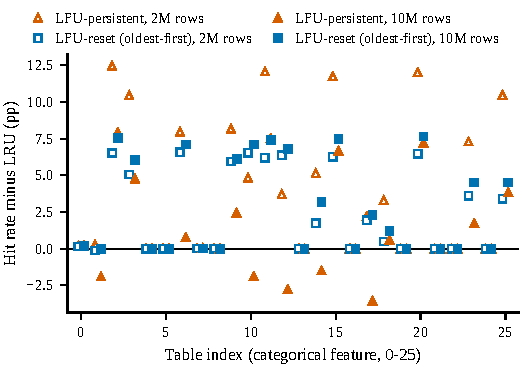
\includegraphics[width=0.6\textwidth]{fig_pertable}
\caption{Per-table caches of \R{sz.256} vectors: hit rate of each LFU variant minus that of LRU, per table, at
\R{lab.2M} (open) and \R{lab.10M} rows (filled) (P3)}
\label{fig:pertable}
\end{figure}

A rank-frequency fit gives Zipf exponents from \R{p3.zipf.lo} to \R{p3.zipf.hi} over the \R{p3.zipf.n} tables that
could be fitted at \R{lab.10M} rows, far from the single exponent assumed earlier. Five tables have at least
\R{p3.large.thr} distinct values on both traces; Fig.~\ref{fig:large} shows them combined: at small capacities
reset-on-eviction LFU, W-TinyLFU and ARC are well above LRU.

\begin{figure}[ht]
\centering
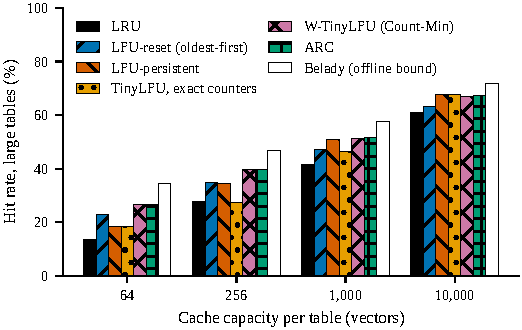
\includegraphics[width=0.55\textwidth]{fig_large}
\caption{Per-table caches, the five large tables combined: hit rate by policy and capacity, first \R{lab.10M} rows
(P3)}
\label{fig:large}
\end{figure}

\section{One cache shared by all tables}
With one shared cache the tables compete for the same entries, and the two LFU variants part ways
(Table~\ref{tab:p3b}, Fig.~\ref{fig:shared}). LFU-reset beats LRU at every shared size on both traces.
LFU-persistent falls below LRU at the smallest size on both traces and at the next size on the longer one, and at the
three smaller sizes it loses more than any other policy from the shorter to the longer trace (\R{p3b.drop.lo} to
\R{p3b.drop.hi} percentage points). Keeping a count for every address therefore does not help a small shared cache;
the cause was not isolated. The five large tables are \R{p3b.large.acc}\% of all accesses at \R{lab.2M} rows but only
\R{p3b.large.hit.lo} to \R{p3b.large.hit.hi}\% of the hits of a \R{sz.256}-entry shared cache. ARC and W-TinyLFU are
the strongest online policies up to \R{sz.1000} shared entries, but their ghost lists, sketch and window would cost
hardware that was not estimated.

\begin{table}[ht]
\centering
\caption{One shared cache: hit rate (\%) at the four capacities, first \R{lab.2M} and \R{lab.10M} rows (P3b, trace
simulation)}
\label{tab:p3b}
\small
\begin{tabular}{@{}lcccccccc@{}}
\toprule
 & \multicolumn{4}{c}{\R{lab.2M} rows} & \multicolumn{4}{c}{\R{lab.10M} rows} \\
\cmidrule(lr){2-5}\cmidrule(lr){6-9}
Policy & \R{sz.256} & \R{sz.1000} & \R{sz.10000} & \R{sz.100000} & \R{sz.256} & \R{sz.1000} & \R{sz.10000} & \R{sz.100000} \\
\midrule
LRU & \R{p3b.2M.256.LRU} & \R{p3b.2M.1000.LRU} & \R{p3b.2M.10000.LRU} & \R{p3b.2M.100000.LRU} & \R{p3b.10M.256.LRU} & \R{p3b.10M.1000.LRU} & \R{p3b.10M.10000.LRU} & \R{p3b.10M.100000.LRU} \\
LFU-reset & \R{p3b.2M.256.LFUr} & \R{p3b.2M.1000.LFUr} & \R{p3b.2M.10000.LFUr} & \R{p3b.2M.100000.LFUr} & \R{p3b.10M.256.LFUr} & \R{p3b.10M.1000.LFUr} & \R{p3b.10M.10000.LFUr} & \R{p3b.10M.100000.LFUr} \\
LFU-persistent & \R{p3b.2M.256.LFUp} & \R{p3b.2M.1000.LFUp} & \R{p3b.2M.10000.LFUp} & \R{p3b.2M.100000.LFUp} & \R{p3b.10M.256.LFUp} & \R{p3b.10M.1000.LFUp} & \R{p3b.10M.10000.LFUp} & \R{p3b.10M.100000.LFUp} \\
W-TinyLFU & \R{p3b.2M.256.WTLFU} & \R{p3b.2M.1000.WTLFU} & \R{p3b.2M.10000.WTLFU} & \R{p3b.2M.100000.WTLFU} & \R{p3b.10M.256.WTLFU} & \R{p3b.10M.1000.WTLFU} & \R{p3b.10M.10000.WTLFU} & \R{p3b.10M.100000.WTLFU} \\
ARC & \R{p3b.2M.256.ARC} & \R{p3b.2M.1000.ARC} & \R{p3b.2M.10000.ARC} & \R{p3b.2M.100000.ARC} & \R{p3b.10M.256.ARC} & \R{p3b.10M.1000.ARC} & \R{p3b.10M.10000.ARC} & \R{p3b.10M.100000.ARC} \\
\bottomrule
\end{tabular}
\end{table}

\begin{figure}[ht]
\centering
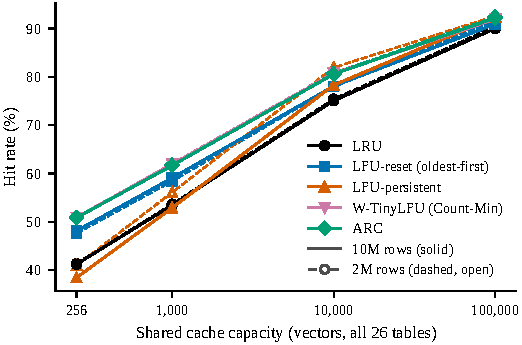
\includegraphics[width=0.5\textwidth]{fig_shared}
\caption{One cache shared by all \R{ds.tables} tables: hit rate against capacity for the five policies of the
shared-cache simulator; \R{lab.10M} rows solid, \R{lab.2M} rows dashed (P3b)}
\label{fig:shared}
\end{figure}

\section{GPU timing without counters}
Phase P4 timed a synthetic model with \R{ds.tables} PyTorch \texttt{EmbeddingBag} tables~\cite{paszke2019pytorch} and
an MLP, in fp32 inference on one H100 and one H200, over table sizes of one and ten million rows, vector dimensions of
\R{p4.dim.lo} and \R{p4.dim.hi}, batches from \R{p4.b.min} to \R{p4.b.max} and five index patterns, using CUDA events
only (\R{p4.cfg} configurations per GPU; on the H100 \R{p4.h100.skip} did not fit in memory). Hardware counters were
not available on either node at the time. A configuration is called launch-bound if its CPU wall time per iteration
is within \R{p4.lb.pct}\% of the value at batch \R{p4.b.min}; there the embedding share (\R{p4.lb.h100.lo} to
\R{p4.lb.h100.hi} on the H100) is a share of kernel-launch time, not of lookup cost (Fig.~\ref{fig:profile}). At
batch \R{p4.b.max} the embedding share of embedding plus MLP time is \R{p4.b8k.h100.lo} to \R{p4.b8k.h100.hi} on
the H100 and \R{p4.b8k.h200.lo} to \R{p4.b8k.h200.hi} on the H200. These timings say nothing about memory
behaviour, which is why P14 used counters.

\begin{figure}[ht]
\centering
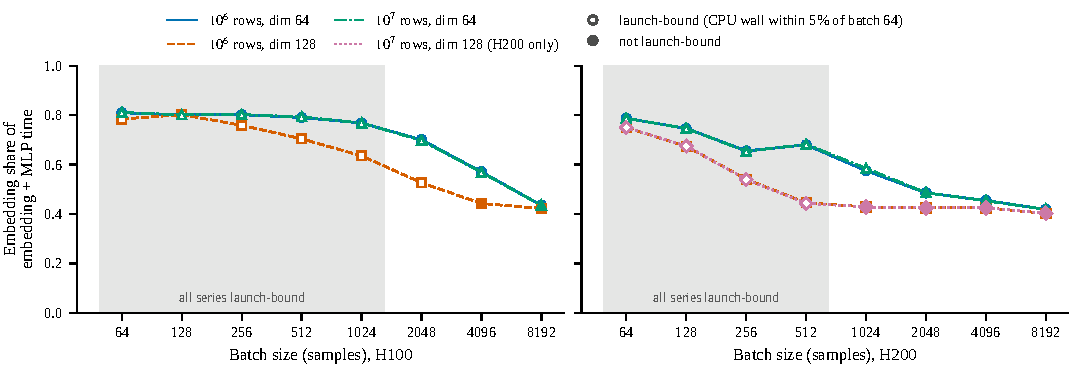
\includegraphics[width=0.9\textwidth]{fig_profile}
\caption{Median embedding share of embedding plus MLP time against batch size, Criteo-hashed indices, fp32
inference on one H100 (left) and one H200 (right), CUDA events only; open markers are launch-bound (P4)}
\label{fig:profile}
\end{figure}

\section{H100 hardware counters on the real stream}
Phase P14 profiled \texttt{nn.EmbeddingBag} with Nsight Compute (version \R{p14.ncu}) on one H100, on the Criteo
stream of the first \R{p14.rows} rows (\R{p14.acc} accesses to \R{p14.uniq} distinct table rows), with
\R{p14.dim}-dimensional fp32 vectors, for one kernel per table and for all tables concatenated, after a warm-up and
over \R{p14.batches} batches per point (Table~\ref{tab:p14}, Fig.~\ref{fig:l2}). The L2 read hit rate falls from
\R{p14.pt.64}\% to \R{p14.pt.16384}\% as the batch grows with one kernel per table, and from \R{p14.cc.64}\% to
\R{p14.cc.16384}\% with the tables concatenated. The profiled window starts at the same row for every batch size, so
batch size and window length change together.

\begin{table}[ht]
\centering
\caption{H100 counters for the embedding kernels, first \R{p14.rows} Criteo rows (P14, Nsight Compute, one GPU)}
\label{tab:p14}
\small
\begin{tabular}{@{}rlrcccc@{}}
\toprule
Batch & Layout & Lookups & L2 hit \% (all) & L2 read hit \% & DRAM bytes / lookup & GPU \textmu s / batch \\
\midrule
\R{p14.B.64} & per table & \R{p14.look.64} & \R{p14.all.64.pt} & \R{p14.pt.64} & \R{p14.dram.64.pt} & \R{p14.us.64.pt} \\
\R{p14.B.64} & concatenated & \R{p14.look.64} & \R{p14.all.64.cc} & \R{p14.cc.64} & \R{p14.dram.64.cc} & \R{p14.us.64.cc} \\
\R{p14.B.1024} & per table & \R{p14.look.1024} & \R{p14.all.1024.pt} & \R{p14.pt.1024} & \R{p14.dram.1024.pt} & \R{p14.us.1024.pt} \\
\R{p14.B.1024} & concatenated & \R{p14.look.1024} & \R{p14.all.1024.cc} & \R{p14.cc.1024} & \R{p14.dram.1024.cc} & \R{p14.us.1024.cc} \\
\R{p14.B.16384} & per table & \R{p14.look.16384} & \R{p14.all.16384.pt} & \R{p14.pt.16384} & \R{p14.dram.16384.pt} & \R{p14.us.16384.pt} \\
\R{p14.B.16384} & concatenated & \R{p14.look.16384} & \R{p14.all.16384.cc} & \R{p14.cc.16384} & \R{p14.dram.16384.cc} & \R{p14.us.16384.cc} \\
\bottomrule
\end{tabular}
\end{table}

\begin{figure}[ht]
\centering
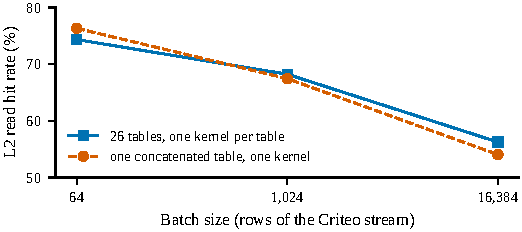
\includegraphics[width=0.5\textwidth]{fig_l2}
\caption{L2 read hit rate of the \texttt{nn.EmbeddingBag} kernels on one H100 against batch size (P14)}
\label{fig:l2}
\end{figure}

For comparison, the trace simulator with one shared cache of \R{p14.cap} vectors, the simulated size closest to the
\R{p14.l2mib}\,MiB L2 at \R{p14.vecbytes} bytes per vector, reaches \R{p3b.2M.100000.LRU}\% with LRU and
\R{p3b.2M.100000.LFUr}\% with LFU-reset over the first \R{lab.2M} rows. The comparison is indicative, not a
validation: the L2 has its own replacement policy, works on sectors (a vector is \R{p14.sectors} of them) and also
holds indices, offsets and outputs, and the counters cover a short window, whereas the simulator counts vector hits
over the whole trace from a cold cache. The H200 node refused counter access with a permission error that needs the
cluster administrators.



\chapter{The RTL Controller and the Tie-Break Finding}\label{ch:rtl}
\section{The v2 controller}
The controller (tag \texttt{rtl-v2-final}, Fig.~\ref{fig:rtl}, Table~\ref{tab:rtlparams}) stores tags, data words,
counters and valid bits in flip-flops, with no SRAM. Each line holds a \R{rtl.vecw}-bit data word, not a full
embedding vector. On a request the FSM goes from IDLE to LOOKUP; the tag compare runs per group on registered copies
of the request address, and a balanced priority tree gives the index of the matching line. On a hit the counter is
incremented and the data returned. On a miss, Stage~A (a minimum tree per group, registered in LOOKUP) and Stage~B
(across groups, in EVICT) find the line with the smallest key $\mathit{eff}$, which is zero for an invalid line and
the count plus one otherwise; FILL installs the returned data.

Phase P1 added the parameter \texttt{COUNTER\_MODE}. In mode 0 (the default) a new tag starts at count one, so the
controller belongs to the LFU-reset family; in mode 1, the original behaviour, the new tag continues from the count
left in the slot; mode 2 (an address-indexed history) stops at elaboration, pending a decision on the counter
scheme. Neither implemented mode keeps a per-address history. The self-checking testbench has \R{rtl.tests} tests;
the P1 mutation check ran \R{p1.mutants} mutants in both modes (\R{p1.runs} runs), and every mutant was killed in the
modes where it can have an effect (\R{p1.survive} runs survive because they change code the mode never executes).

\begin{table}[ht]
\centering
\caption{Controller parameters (\protect\path{results/P7/TABLES.md}, from \protect\path{rtl/v2})}
\label{tab:rtlparams}
\begin{tabular}{@{}ll@{}}
\toprule
Parameter & Value \\
\midrule
Address width (bits) & \R{rtl.addrw} \\
Data word (bits) & \R{rtl.vecw} \\
Counter width (bits), saturation & \R{rtl.cntw}, \R{rtl.sat} \\
Groups for victim selection & \R{rtl.groups} \\
Depths built (lines) & \R{sz.16}, \R{sz.64}, \R{sz.256} \\
Trace-simulator LFU counter cap & \R{rtl.simcap} \\
\bottomrule
\end{tabular}
\end{table}

\begin{figure}[ht]
\centering
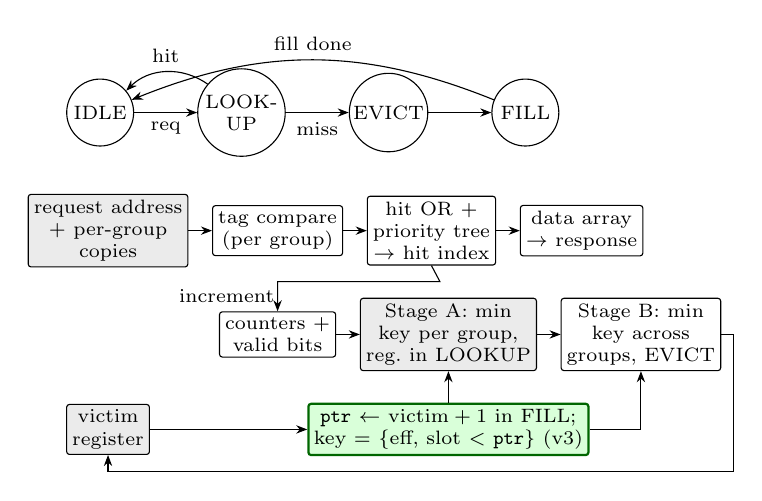
\begin{tikzpicture}[
  font=\scriptsize, >={Stealth[length=4pt]},
  blk/.style={draw, rounded corners=1pt, align=center, minimum height=5.5mm, inner sep=2pt, fill=white},
  st/.style={draw, circle, inner sep=1pt, minimum size=8.5mm, align=center},
  reg/.style={blk, fill=black!8},
  new/.style={blk, fill=green!15, draw=green!40!black, thick}]
  \node[st] (idle) {IDLE};
  \node[st, right=8mm of idle] (look) {LOOK-\\UP};
  \node[st, right=8mm of look] (evict) {EVICT};
  \node[st, right=8mm of evict] (fill) {FILL};
  \draw[->] (idle) -- node[below]{req} (look);
  \draw[->] (look) -- node[below]{miss} (evict);
  \draw[->] (evict) -- (fill);
  \draw[->] (look) to[bend right=40] node[above]{hit} (idle);
  \draw[->] (fill) to[bend right=22] node[above]{fill done} (idle);
  \node[reg, below=6mm of idle, xshift=1mm] (addr) {request address\\+ per-group\\copies};
  \node[blk, right=3mm of addr] (cmp) {tag compare\\(per group)};
  \node[blk, right=3mm of cmp] (hit) {hit OR +\\priority tree\\$\rightarrow$ hit index};
  \node[blk, right=3mm of hit] (data) {data array\\$\rightarrow$ response};
  \node[blk, below=7mm of cmp] (cnt) {counters +\\valid bits};
  \node[reg, right=3mm of cnt] (sa) {Stage A: min\\key per group,\\reg.\ in LOOKUP};
  \node[blk, right=3mm of sa] (sb) {Stage B: min\\key across\\groups, EVICT};
  \node[new, below=4mm of sa] (ptr) {\texttt{ptr} $\leftarrow$ victim${}+1$ in FILL;\\key $=$ \{eff, slot $<$ \texttt{ptr}\} (v3)};
  \node[reg] (vic) at (addr |- ptr) {victim\\register};
  \draw[->] (addr) -- (cmp);
  \draw[->] (cmp) -- (hit);
  \draw[->] (hit) -- (data);
  \draw[->] (cnt) -- (sa);
  \draw[->] (sa) -- (sb);
  \draw[->] (vic.east) -- (ptr.west);
  \draw[->] (ptr.north) -- (sa.south);
  \draw[->] (ptr.east) -| (sb.south);
  \draw[->] (sb.east) -- ++(1.5mm,0) |- ($(ptr.south)+(0,-2mm)$) -| (vic.south);
  \coordinate (mid) at ($(hit.south)!0.5!(sa.north)$);
  \draw[->] (hit.south) -- (mid) -| node[pos=0.75, left, inner sep=1pt]{increment} (cnt.north);
\end{tikzpicture}
\caption{The controller: FSM (top) and datapath (bottom; grey blocks are registers). Green: the Rotate-victim change
of v3 (pointer register and one wrap bit in the tree key)}
\label{fig:rtl}
\end{figure}

Both minimum trees keep their left operand unless the right one is strictly smaller, so among lines with the smallest
count the victim is the one with the \emph{lowest slot index}. The simulator of Chapter~\ref{ch:policy} instead
evicts the entry installed earliest, and its counters saturate at a higher value. Whether these differences matter
was the question of phases P8 and P9.

\section{The RTL-exact simulator}
While preparing the power analysis (P8), the hit counts of the RTL on two slices of the shared stream did not match
what the simulated policy predicted. Phase P9 therefore wrote a trace-simulator policy that models the RTL exactly:
slots, lowest-index filling of invalid lines, the key $\mathit{eff}$, the lowest-slot victim, the install count of each
mode and saturation at \R{rtl.sat}. It was validated against the RTL hit flag request by request in \R{p9.runs}
zero-delay RTL simulations (three depths, both modes, two cold-start slices of \R{p9.slicereq} consecutive requests,
called \emph{row0} and \emph{row1M}, and prefixes of them), with \R{p9.mism} mismatches in \R{p9.req} requests. For the
ablation, three variants of LFU-reset were built: with lowest-slot ties, with \R{rtl.cntw}-bit counters, and with
both; the last equals the RTL-exact policy in mode 0.

\section{The controller loses to LRU}
On the full shared-cache traces, the RTL-exact policy in mode 0 (the \emph{v2 rule}) is below LRU at all four sizes
simulated from \R{sz.256} to \R{sz.100000} entries, on both traces (Table~\ref{tab:p9}, Fig.~\ref{fig:tiebreak}). At
the two smallest sizes simulated (phase P11), where LRU is low, the v2 rule is above LRU but far below LFU-reset.
Mode 1 is no remedy: it beats LRU at \R{sz.256} entries but loses at \R{sz.1000} and \R{sz.10000} entries on both
traces.

\begin{table}[ht]
\centering
\caption{One shared cache, first \R{lab.10M} rows: hit rate (\%) and the v2 rule against LRU (P9, P11, trace
simulation; n/r: not run)}
\label{tab:p9}
\small
\begin{tabular}{@{}rcccccrr@{}}
\toprule
Entries & LRU & LFU-reset & v2 rule & mode 1 & v3 rule & v2 rule $-$ LRU (hits) & gap to LFU-reset (hits) \\
\midrule
\R{sz.16} & \R{p9t.16.LRU} & \R{p9t.16.LFUr} & \R{p9t.16.v2} & n/r & \R{p9t.16.v3} & & \\
\R{sz.64} & \R{p9t.64.LRU} & \R{p9t.64.LFUr} & \R{p9t.64.v2} & n/r & \R{p9t.64.v3} & & \\
\R{sz.256} & \R{p9t.256.LRU} & \R{p9t.256.LFUr} & \R{p9t.256.v2} & \R{p9t.256.m1} & \R{p9t.256.v3} & \R{p9t.256.vslru} & \R{p9t.256.gap} \\
\R{sz.1000} & \R{p9t.1000.LRU} & \R{p9t.1000.LFUr} & \R{p9t.1000.v2} & \R{p9t.1000.m1} & \R{p9t.1000.v3} & \R{p9t.1000.vslru} & \R{p9t.1000.gap} \\
\R{sz.10000} & \R{p9t.10000.LRU} & \R{p9t.10000.LFUr} & \R{p9t.10000.v2} & \R{p9t.10000.m1} & \R{p9t.10000.v3} & \R{p9t.10000.vslru} & \R{p9t.10000.gap} \\
\R{sz.100000} & \R{p9t.100000.LRU} & \R{p9t.100000.LFUr} & \R{p9t.100000.v2} & \R{p9t.100000.m1} & \R{p9t.100000.v3} & \R{p9t.100000.vslru} & \R{p9t.100000.gap} \\
\bottomrule
\end{tabular}
\end{table}

\begin{figure}[ht]
\centering
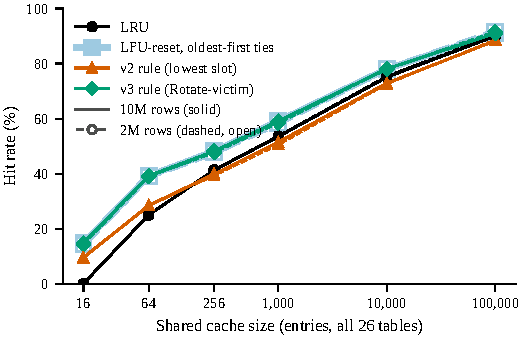
\includegraphics[width=0.55\textwidth]{fig_tiebreak}
\caption{One shared cache: hit rate against size for LRU, oldest-first LFU-reset, the v2 rule and the v3 rule;
\R{lab.10M} rows solid, \R{lab.2M} dashed. The v3 rule lies on LFU-reset (P9, P11)}
\label{fig:tiebreak}
\end{figure}

\section{Mechanism and ablation}
A new tag takes the slot of the victim, which was the lowest-indexed slot with the minimum count, and starts at count
one; unless it is hit before the next miss, it is again the lowest-indexed minimum and is evicted next. On the row0
slice at \R{sz.256} entries the v2 rule evicts the line installed by the previous miss in \R{p9.prev.v2} of its
\R{p9.prev.v2.n} evictions; oldest-first LFU-reset does so in \R{p9.prev.old} of \R{p9.prev.old.n}. The ablation
confirms the cause: LFU-reset with lowest-slot ties alone gives exactly the hits of the RTL-exact policy, and
LFU-reset with \R{rtl.cntw}-bit counters alone gives exactly the hits of LFU-reset, at all four sizes and on both
traces. The tie-break accounts for the whole gap to oldest-first LFU-reset (last column of Table~\ref{tab:p9}),
saturation for \R{p9.sat} hits and their interaction for \R{p9.int}.

The argument needs only that new lines start at the minimum count, that they take the victim's slot, that counts do
not decrease between misses, and that ties are broken by a fixed index order. Comparator trees and priority encoders give such a fixed order unless extra state is added, so the mechanism can arise in other counter-based caches built this way. Whether it costs hit rate there depends on the workload and the cache size; it was measured only for this controller on Criteo, and at \R{sz.16} and \R{sz.64} entries the v2 rule still beats LRU.

\section{Candidate fixes}
Three replacements for the lowest-slot rule were simulated (Table~\ref{tab:cand}): \emph{Rotate-victim}, which starts
the search at the slot after the previous victim; \emph{Rotate-step}, whose pointer advances on every miss; and a
\emph{young bit} per line. At depth \R{sz.256} the first two add \R{p9.ff.rs} flip-flops and the third
\R{p9.ff.yb}. In mode 0, Rotate-victim recovers the whole gap to one decimal at every size, the young bit recovers nearly all of it (Table~\ref{tab:cand}), and Rotate-step recovers more than the gap at most sizes because it gets more hits than LFU-reset. Rotate-victim was
chosen because it reproduces the policy the controller was written for: on the slices it gives exactly the hits of
oldest-first LFU-reset, and on \R{p9.probe.n} synthetic traces it departs from it on \R{p9.probe.rv}, against
\R{p9.probe.rs} for Rotate-step. In mode 1 every candidate loses hits against the unchanged rule (negative recovered
share), so the fix changes mode 0 only.

\begin{table}[ht]
\centering
\caption{Candidate tie-break rules: share of the gap between the RTL-exact policy and oldest-first LFU-reset that
each recovers (\%), one shared cache, first \R{lab.10M} rows (P9, trace simulation only)}
\label{tab:cand}
\begin{tabular}{@{}rcccc@{}}
\toprule
Entries & Rotate-victim, mode 0 & Rotate-step, mode 0 & Young bit, mode 0 & Rotate-victim, mode 1 \\
\midrule
\R{sz.256} & \R{p9c.256.rv} & \R{p9c.256.rs} & \R{p9c.256.yb} & \R{p9c.256.rv1} \\
\R{sz.1000} & \R{p9c.1000.rv} & \R{p9c.1000.rs} & \R{p9c.1000.yb} & \R{p9c.1000.rv1} \\
\R{sz.10000} & \R{p9c.10000.rv} & \R{p9c.10000.rs} & \R{p9c.10000.yb} & \R{p9c.10000.rv1} \\
\R{sz.100000} & \R{p9c.100000.rv} & \R{p9c.100000.rs} & \R{p9c.100000.yb} & \R{p9c.100000.rv1} \\
\bottomrule
\end{tabular}
\end{table}

\section{Rotate-victim in RTL (v3)}
Phase P10 added to \texttt{rtl/v3} a pointer register \texttt{ptr} that loads victim${}+1$ (modulo the depth) when a
fill completes, and extended both tree keys by one wrap bit, set when the slot index is below \texttt{ptr}, so the
victim is the first minimum-count slot at or after \texttt{ptr}, wrapping around (key width \R{p10.kw} bits). Tree
depth, counters and FSM are unchanged, and mode 1 keeps the v2 rule. A new tie-order test checks the victim order and
the wrap-around; the \R{p10.mut} mutants of the new rule are all caught by it.

In lockstep with the simulator, the v3 RTL shows \R{p10.mism} mismatches, request by request, in all \R{p10.runs}
runs (three depths, both modes, both slices); Table~\ref{tab:p10} gives the hits in mode 0. In mode 1 the v3 hit logs
equal those of v2 line for line. On these cold-start slices Rotate-victim gives more hits than the v2 rule at depths
\R{sz.64} and \R{sz.256}, and fewer at depth \R{sz.16}.

\begin{table}[ht]
\centering
\caption{RTL lockstep with the simulator, mode 0, slices of \R{p9.slicereq} requests from a cold start (P10)}
\label{tab:p10}
\begin{tabular}{@{}rlrr@{}}
\toprule
Depth & Slice & v3 RTL hits (= model) & v2-rule hits \\
\midrule
\R{sz.16} & row0 & \R{p10.16.row0.v3} & \R{p10.16.row0.v2} \\
\R{sz.16} & row1M & \R{p10.16.row1M.v3} & \R{p10.16.row1M.v2} \\
\R{sz.64} & row0 & \R{p10.64.row0.v3} & \R{p10.64.row0.v2} \\
\R{sz.64} & row1M & \R{p10.64.row1M.v3} & \R{p10.64.row1M.v2} \\
\R{sz.256} & row0 & \R{p10.256.row0.v3} & \R{p10.256.row0.v2} \\
\R{sz.256} & row1M & \R{p10.256.row1M.v3} & \R{p10.256.row1M.v2} \\
\bottomrule
\end{tabular}
\end{table}

On the full traces (P9, P11), Rotate-victim in mode 0 recovers \R{p9.rec}\% of the gap at every size, to one decimal,
differs from oldest-first LFU-reset by at most \R{p9.rvdiff.hi.abs} hits, and equals it exactly, in total and in every
table, at \R{sz.16}, \R{sz.64} and \R{sz.256} entries. At \R{sz.256} entries on the longer trace it is \R{d.v3lru}
points above LRU and \R{d.v3v2} above the v2 rule. The gain is not uniform: inside the shared cache \R{p11.tl.16} of
the \R{ds.tables} tables have fewer hits under v3 than under v2 at \R{sz.16} entries, and \R{p11.tl.256} at
\R{sz.256}.

\section{Verification summary}
Table~\ref{tab:verif} lists the checks of v2 and v3. Yosys proves the v2 and v3 RTL equivalent in mode 1 at depths
\R{sz.16} and \R{sz.64}; the proof was not run at depth \R{sz.256} and does not cover the netlists. The gate-level checks of Chapters~\ref{ch:open} and~\ref{ch:c2} compare every simulated netlist with its RTL cycle by cycle; the simulated netlists are those listed in Table~\ref{tab:verif}.

\begin{table}[ht]
\centering
\caption{Verification of the controller, as run}
\label{tab:verif}
\small
\begin{tabularx}{\textwidth}{@{}>{\raggedright\arraybackslash}p{0.33\textwidth}L@{}}
\toprule
Check & Scope and result \\
\midrule
RTL-exact model against v2 RTL (P9) & \R{p9.runs} runs (three depths, both modes, two slices, full and prefix):
\R{p9.mism} mismatches in \R{p9.req} requests \\
v3 RTL against the simulator (P10) & \R{p10.runs} runs of \R{p9.slicereq} requests (Rotate-victim in mode 0, v2 rule in
mode 1): \R{p10.mism} mismatches \\
Mutation suite on the final v2 RTL (P5d) & \R{p5.mut.tb} killed by the testbench, \R{p5.mut.ls} by lockstep,
\R{p5.mut.eq} equivalent \\
Mutation suite on v3 (P11) & \R{p11.mut.tb} killed by the testbench, \R{p11.mut.ls} by lockstep; no non-equivalent
mutant survives \\
v2 and v3 equal in mode 1 (P11, Yosys, RTL only) & proven at depth \R{sz.16} (\R{p11.eq.16} cells) and \R{sz.64}
(\R{p11.eq.64} cells); not run at \R{sz.256} \\
Open-flow GLS of v2 (P5f), zero delay & \R{p5f.netlists} netlists, \R{p5f.cycles} random cycles each:
\R{p5f.mism} mismatching cycles \\
Open-flow GLS of v3 (P11), zero delay & \R{p11.gls.n} netlist runs on the slices: \R{p11.gls.mism} mismatching cycles \\
28nm GLS before layout (P13) & zero delay and SDF, v2 and v3, two slices: \R{p13.mism} mismatching cycles \\
28nm GLS after routing (P15) & zero delay and SDF: \R{p15.mism} mismatching cycles; SDF path delays
\R{p15.sdf.path}\%, timing checks \R{p15.sdf.check}\% annotated \\
\bottomrule
\end{tabularx}
\end{table}

\chapter{Open-Source Implementation Flow}\label{ch:open}
\section{Flow}
Phases P5 to P8 used open tools only: Yosys \R{tool.yosys} with ABC~\cite{wolf_yosys,brayton2010abc} to map the RTL to
the NanGate45 open library~\cite{nangate45} (typical corner), OpenSTA \R{tool.opensta}~\cite{opensta} with the
library's wire-load model and an ideal clock for setup and hold, and Icarus Verilog~\cite{icarus} for simulation.
NanGate45 is an open library for a generic predictive process; all results are pre-layout, and area is the sum of
cell areas. Each configuration (depths \R{sz.16}, \R{sz.64} and \R{sz.256}; mode 0 and mode 1) was synthesised for a \R{clk.1000}\,MHz
and a \R{clk.500}\,MHz target, and Fmax is the reciprocal of the clock period minus the worst setup slack.

\section{Baseline and timing restructuring}
The baseline (P5, tag \texttt{rtl-v2-baseline}) met neither target. Three RTL changes replaced serial loops by balanced trees (Table~\ref{tab:p5iter},
Fig.~\ref{fig:fmax}): a Stage-B tree with per-group copies of the request address (P5b), a Stage-A tree (P5c) and a
hit-index priority tree (P5d, tag \texttt{rtl-v2-final}). For P5c a rule was fixed before synthesis: keep the address
copies only if, at depth \R{sz.256}, Fmax with copies is at least \R{p5c.rule} times Fmax without them; the copies gave
\R{p5c.copy.m0}\% and \R{p5c.copy.m1}\% and were kept. Every change was checked by the unchanged unit tests and by
lockstep against the earlier versions, with no port or victim mismatch.

\begin{table}[ht]
\centering
\caption{Pre-layout Fmax (MHz) on NanGate45, mode 0, \R{clk.1000}\,MHz netlists, by design iteration, and the spread of Fmax over
eight designs with identical logic (flow noise) (P5 to P5e)}
\label{tab:p5iter}
\begin{tabular}{@{}lccc@{}}
\toprule
Iteration & Depth \R{sz.16} & Depth \R{sz.64} & Depth \R{sz.256} \\
\midrule
P5 baseline & \R{p5.f.16} & \R{p5.f.64} & \R{p5.f.256} \\
P5b Stage-B tree and address copies & \R{p5b.f.16} & \R{p5b.f.64} & \R{p5b.f.256} \\
P5c Stage-A tree & \R{p5c.f.16} & \R{p5c.f.64} & \R{p5c.f.256} \\
P5d hit-index tree (old flow) & \R{p5d.f.16} & \R{p5d.f.64} & \R{p5d.f.256} \\
P5e same RTL, timing-driven flow & \R{p5e.f.16} & \R{p5e.f.64} & \R{p5e.f.256} \\
\midrule
Flow noise, old flow (\%) & \R{p5d.noise.16.0} & \R{p5d.noise.64.0} & \R{p5d.noise.256.0} \\
Flow noise, timing-driven flow (\%) & \R{p5e.noise.16.0} & \R{p5e.noise.64.0} & \R{p5e.noise.256.0} \\
\bottomrule
\end{tabular}
\end{table}

\begin{figure}[ht]
\centering
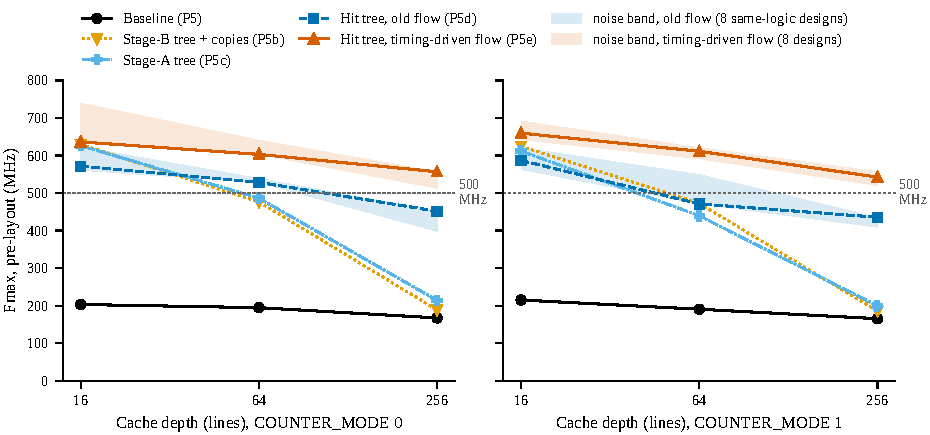
\includegraphics[width=0.9\textwidth]{fig_fmax}
\caption{Pre-layout Fmax on NanGate45 of the \R{clk.1000}\,MHz netlists against depth for each design iteration; shaded: the
Fmax range of eight designs with identical logic (flow noise) for the two flows (P5 to P5e)}
\label{fig:fmax}
\end{figure}

The noise floor matters more than any single number. P5d synthesised eight designs with the same logic (the final RTL,
a flat-vector form of it, and three one-line rewrites of each); the flow alone moves their Fmax by up to
\R{p5d.noise.64.1}\%. Differences between two designs smaller than this spread are not evidence of a design effect.
The first form of the hit-index tree, written with flat vectors, took Icarus \R{p5d.icarus}\,s per depth-\R{sz.256} lockstep
run and was rewritten with arrays of the same logic.

\section{Timing-driven flow}
P5e found why the \R{clk.1000}\,MHz and \R{clk.500}\,MHz netlists were often identical: the delay target passed to ABC could not bind
when ABC's own estimate was above both targets, and ABC's timer ran without the wire-load model and without the
flip-flop clock-to-output and setup times, so it was optimistic. The new flow runs three delay-oriented ABC passes and
buffering and sizing with the wire-load model, with an ABC target of the period minus \R{p5e.budget}\,ps. On the same
RTL it raises Fmax beyond the noise band at every depth (Table~\ref{tab:p5e}); the \R{clk.500}\,MHz netlists meet timing at
depths \R{sz.16} and \R{sz.64}, and miss it at depth \R{sz.256} by amounts far inside the noise, so whether depth
\R{sz.256} meets \R{clk.500}\,MHz is not demonstrated either way.

\begin{table}[ht]
\centering
\caption{Final v2 controller on NanGate45, timing-driven flow, pre-layout (P5e); Fmax from the \R{clk.1000}\,MHz netlists; last
column: worst setup slack of the netlist synthesised for \R{clk.500}\,MHz}
\label{tab:p5e}
\begin{tabular}{@{}rrrrrrr@{}}
\toprule
Depth & & Cells & Flip-flops & Area (\umsq) & Fmax (MHz) & WNS at \R{clk.500}\,MHz (ns) \\
\midrule
\R{sz.16} & mode 0 & \R{p5e.16.0.cells} & \R{p5e.16.0.ff} & \R{p5e.16.0.area} & \R{p5e.16.0.fmax} & \R{p5e.16.0.wns500} \\
\R{sz.16} & mode 1 & \R{p5e.16.1.cells} & \R{p5e.16.1.ff} & \R{p5e.16.1.area} & \R{p5e.16.1.fmax} & \R{p5e.16.1.wns500} \\
\R{sz.64} & mode 0 & \R{p5e.64.0.cells} & \R{p5e.64.0.ff} & \R{p5e.64.0.area} & \R{p5e.64.0.fmax} & \R{p5e.64.0.wns500} \\
\R{sz.64} & mode 1 & \R{p5e.64.1.cells} & \R{p5e.64.1.ff} & \R{p5e.64.1.area} & \R{p5e.64.1.fmax} & \R{p5e.64.1.wns500} \\
\R{sz.256} & mode 0 & \R{p5e.256.0.cells} & \R{p5e.256.0.ff} & \R{p5e.256.0.area} & \R{p5e.256.0.fmax} & \R{p5e.256.0.wns500} \\
\R{sz.256} & mode 1 & \R{p5e.256.1.cells} & \R{p5e.256.1.ff} & \R{p5e.256.1.area} & \R{p5e.256.1.fmax} & \R{p5e.256.1.wns500} \\
\bottomrule
\end{tabular}
\end{table}

\section{Gate-level simulation and equivalence}
Phase P5f simulated the \R{p5f.netlists} netlists (three depths, both modes, both targets) with zero delay. The cell
models were generated by Yosys from the library and checked against the library's cell functions: \R{p5f.pass} of
\R{p5f.cells} passed, and the one failure is a flip-flop with both set and reset that no netlist uses. In lockstep with
the RTL over \R{p5f.cycles} random cycles each, comparing the hit flag, response valid, response data, fill request and
fill address every cycle, all netlists show \R{p5f.mism} mismatching cycles and no unknown value on any output, and the
unit tests pass on the netlists. Yosys proves the four depth-\R{sz.16} netlists equivalent to the RTL (\R{p5f.eq} equivalence
cells); the proof treats the asynchronous reset as synchronous and was completed at depth \R{sz.16} only.

\section{Mutation testing and counter saturation}
Mutation testing checks that the tests can fail: each mutant is a deliberately broken copy of the RTL, and the suite
must kill every mutant that changes behaviour. For the final v2 RTL the unit testbench killed \R{p5.mut.tb} mutant
runs and the lockstep check \R{p5.mut.ls} more, and \R{p5.mut.eq} runs were of equivalent mutants. Some mutants, such
as reversing the tie order of a tree, pass the unit tests (any fixed order looks the same at the ports) and are caught
only by the lockstep comparison of the victim slot. To see whether the random stimulus exercised counter saturation,
the RTL was rerun on the same stimulus with the counters recorded: a line held the maximum count in \R{p7.sat.cyc.lo}
to \R{p7.sat.cyc.hi} of the cycles, and \R{p7.sat.sup.lo} to \R{p7.sat.sup.hi} hit increments were suppressed at the
maximum.

\section{Power analysis and its limits}
Phase P8 ran OpenSTA power analysis on the \R{clk.500}\,MHz netlists with switching activity from zero-delay gate-level
simulation (Table~\ref{tab:p8}). The clock-pin energy of the flip-flops dominates every configuration: each flip-flop
spends nearly the same recalculated energy on its clock pin in every cycle and configuration (\R{p8.ckff}\,fJ per cycle at depth \R{sz.256}). OpenSTA weights the clock-pin energy by state probabilities that it assumes independent; in one test on one netlist, a per-event recomputation from the activity file differed from OpenSTA by \R{p8.bias}\%, so the clock-pin term in
Table~\ref{tab:p8} is the recalculated one. The numbers are labelled NanGate45, typical corner, pre-layout, no clock
tree, flip-flop storage, random fill data, and activity over \R{p8.cycles} cycles of the row0 slice; they are not
comparable with the 28nm results of Chapter~\ref{ch:c2}.

\begin{table}[ht]
\centering
\caption{Power components per clock cycle (pJ, leakage in mW), NanGate45, \R{clk.500}\,MHz netlists, mode 0, row0 slice,
pre-layout, no clock tree (P8)}
\label{tab:p8}
\small
\begin{tabular}{@{}rccccc@{}}
\toprule
Depth & Flip-flop clock pins & Other flip-flop & Combinational & Switching & Leakage (mW) \\
\midrule
\R{sz.16} & \R{p8.16.ck} & \R{p8.16.ffo} & \R{p8.16.comb} & \R{p8.16.sw} & \R{p8.16.leak} \\
\R{sz.64} & \R{p8.64.ck} & \R{p8.64.ffo} & \R{p8.64.comb} & \R{p8.64.sw} & \R{p8.64.leak} \\
\R{sz.256} & \R{p8.256.ck} & \R{p8.256.ffo} & \R{p8.256.comb} & \R{p8.256.sw} & \R{p8.256.leak} \\
\bottomrule
\end{tabular}
\end{table}

\section{The v3 controller on the open flow}
Phase P11 synthesised v3 with the P5e flow unchanged. Every Fmax change of v3 in mode 0 lies within the
\R{p11.nnoise}\% change seen between the two versions in mode 1, whose logic is unchanged, so no Fmax cost or gain of
Rotate-victim is claimed from this flow. The flip-flop count in mode 0 grows by exactly the pointer width
(\R{p11.ff.256} at depth \R{sz.256}).

\chapter{Commercial 28nm FD-SOI Flow}\label{ch:c2}
\section{Flow and confidentiality}
Phases P12 to P16 used an STMicroelectronics 28nm FD-SOI standard-cell library (accessed through CMP) on a laboratory server (C2) reachable only from the laboratory network, with Cadence Genus for synthesis and power, Xcelium for
gate-level simulation and Innovus for place and route (Table~\ref{tab:flows}). The library is licensed: its files never
leave the server, are never read or printed, and the repository holds only aggregate tables generated from the tool reports of the project's own runs; their publication was approved by Prof.\ Mane. Genus states no area unit in its reports, so synthesis
areas are in library units; Innovus reports \umsq. Each design point was run once.

\begin{table}[ht]
\centering
\caption{Commercial flows and settings (tt: typical corner)}
\label{tab:flows}
\small
\begin{tabularx}{\textwidth}{@{}>{\raggedright\arraybackslash}p{0.2\textwidth}L@{}}
\toprule
Flow & Settings \\
\midrule
Synthesis (P12) & Genus, tt; library default (zero) wire load, no parasitics, pre-layout; I/O delay
\R{p12.io}${}\times{}$period; periods \R{p12.per.min} to \R{p12.per.max} ns \\
GLS and power (P13, P15) & Xcelium, \R{p13.req} requests per slice, two slices, netlist and RTL compared every
cycle; zero delay and SDF (path delays); Genus power with the activity file of the SDF run \\
Place and route (P15) & Innovus, tt (\R{p15.tt.v}\,V, \R{p15.tt.t}\,\textdegree C, nominal RC); end caps, well taps,
four-net power grid; multi-row cells excluded; setup target slack \R{p15.tslack} ns, extra post-route setup
optimisation, two post-route hold passes at \R{p15.met} and \R{p15.fail} ns; parasitics extracted for power \\
Corners (P16) & Routed layouts re-timed, no re-optimisation: slow (\R{p16.ss.v}\,V, \R{p16.ss.t}\,\textdegree C,
maximum-RC extraction), fast (\R{p16.ff.v}\,V, \R{p16.ff.t}\,\textdegree C, minimum-C extraction); on-chip
variation \\
\bottomrule
\end{tabularx}
\end{table}

\section{Synthesis brackets and area noise}
Genus synthesised v2 and v3 in both modes at all three depths for six clock periods. Because the Fmax of a failing run
depends on its target period, the reliable figure is the bracket: the tightest period met and the loosest period
failed (Table~\ref{tab:p12}). At depths \R{sz.16} and \R{sz.256} the brackets agree for all four version and mode
pairs, and at depth \R{sz.64} for all but v3 in mode 1. Since the logic of mode 1 is the same in both versions, the
v3$-$v2 differences in mode 1 are the observed noise of the flow: at a relaxed \R{p12.relax} ns the area of v3 differs
from v2 by at most \R{p12.a.16.m0.abs}\% in mode 0, while the differences in mode 1 reach \R{p12.a.256.m1.abs}\%, and at
tight periods the same-logic area difference reaches \R{p12.noise}\%.

\begin{table}[ht]
\centering
\caption{Genus synthesis, typical corner, pre-layout: tightest period met / loosest period failed (ns) (P12)}
\label{tab:p12}
\begin{tabular}{@{}llccc@{}}
\toprule
Version & & Depth \R{sz.16} & Depth \R{sz.64} & Depth \R{sz.256} \\
\midrule
v2 & mode 0 & \R{p12.b.v2.0.16.met} / \R{p12.b.v2.0.16.fail} & \R{p12.b.v2.0.64.met} / \R{p12.b.v2.0.64.fail} & \R{p12.b.v2.0.256.met} / \R{p12.b.v2.0.256.fail} \\
v2 & mode 1 & \R{p12.b.v2.1.16.met} / \R{p12.b.v2.1.16.fail} & \R{p12.b.v2.1.64.met} / \R{p12.b.v2.1.64.fail} & \R{p12.b.v2.1.256.met} / \R{p12.b.v2.1.256.fail} \\
v3 & mode 0 & \R{p12.b.v3.0.16.met} / \R{p12.b.v3.0.16.fail} & \R{p12.b.v3.0.64.met} / \R{p12.b.v3.0.64.fail} & \R{p12.b.v3.0.256.met} / \R{p12.b.v3.0.256.fail} \\
v3 & mode 1 & \R{p12.b.v3.1.16.met} / \R{p12.b.v3.1.16.fail} & \R{p12.b.v3.1.64.met} / \R{p12.b.v3.1.64.fail} & \R{p12.b.v3.1.256.met} / \R{p12.b.v3.1.256.fail} \\
\bottomrule
\end{tabular}
\end{table}

Genus merged the per-group copies of the request address into one register, so the normal netlists lack the fan-out
split the RTL was written for. Keeping all of them (\R{p12.copies} flip-flops, \emph{merge-off}) raised the Fmax of
the failing \R{p12.br.256.fail} ns runs at depth \R{sz.256} from \R{p12.f.v2} to \R{p12.fmo.v2}\,MHz for v2
(\R{p12.mo.v2}\%) and from \R{p12.f.v3} to \R{p12.fmo.v3}\,MHz for v3 (\R{p12.mo.v3}\%), one run each. In those
failing runs the option costs v3 \R{p12.mo.a.v3.abs}\% in area, more than any same-logic difference, and v2
\R{p12.fmo.a.v2}\%; in the netlists synthesised at \R{p13.period} ns, which go to gate-level simulation and layout, it
costs v3 \R{p12.mo.a08.v3.abs}\%.

\section{Gate-level simulation and energy before layout}
The merge-off depth-\R{sz.256} netlists of v2 and v3, synthesised at \R{p13.period} ns, were simulated in lockstep with their
RTL on both slices, with zero delay and with SDF path delays: no mismatching cycle and no unknown value
(Table~\ref{tab:verif}). The SDF runs annotate the path delays but none of the timing checks, because the cell models'
checks are conditional and the SDF written by Genus has no conditions; \R{p13.variants} variants of the SDF writer
were tried, all without timing checks. Power was computed by Genus with the switching activity of the SDF runs, and
energy per request as power times cycles times period over the number of requests (Table~\ref{tab:p13}). v3 needs
\R{p13.dE.row1M.abs} to \R{p13.dE.row0.abs}\% less energy per request than v2: its power is slightly higher, but with
more hits fewer requests wait for a fill and the run takes fewer cycles. Flip-flop outputs and ports are fully
annotated, combinational driver nets only in part; combinational logic is at most \R{p13.logic.hi}\% of the power,
and its share is taken as the bound on the activity error.

\begin{table}[ht]
\centering
\caption{Gate-level power and energy before layout, merge-off depth-\R{sz.256} netlists, mode 0, \R{p13.period} ns,
typical corner, no clock tree (P13)}
\label{tab:p13}
\small
\begin{tabular}{@{}llccccc@{}}
\toprule
Version & Slice & Power (mW) & Energy (pJ/req.) & Registers (\%) & Logic (\%) & Driver nets (\%) \\
\midrule
v2 & row0 & \R{p13.mW.v2.row0} & \R{p13.E.v2.row0} & \R{p13.reg.v2.row0} & \R{p13.logic.v2.row0} & \R{p13.cov.v2.row0} \\
v2 & row1M & \R{p13.mW.v2.row1M} & \R{p13.E.v2.row1M} & \R{p13.reg.v2.row1M} & \R{p13.logic.v2.row1M} & \R{p13.cov.v2.row1M} \\
v3 & row0 & \R{p13.mW.v3.row0} & \R{p13.E.v3.row0} & \R{p13.reg.v3.row0} & \R{p13.logic.v3.row0} & \R{p13.cov.v3.row0} \\
v3 & row1M & \R{p13.mW.v3.row1M} & \R{p13.E.v3.row1M} & \R{p13.reg.v3.row1M} & \R{p13.logic.v3.row1M} & \R{p13.cov.v3.row1M} \\
\bottomrule
\end{tabular}
\end{table}

\section{Place and route}
The floorplan has end caps on the row ends, well taps placed in a checkerboard, and a four-net power grid: supply,
ground and the two body-bias nets of FD-SOI, which connect to the well taps. The first flow left power-rail shorts in the depth-\R{sz.256} designs, at every instance of the one double-height cell type, most of them inserted during optimisation (\R{p15.sh.v2.08} and \R{p15.sh.v2.09} shorting instances for v2 at \R{p13.period} and \R{p15.fail} ns, \R{p15.sh.v3.08} and \R{p15.sh.v3.09} for v3). The
fix set all \R{p15.dontuse} multi-row cells of the library as not to be used and resized the multi-row instances of
the netlists (\R{p15.rs.v2} in v2, \R{p15.rs.v3} in v3) before the floorplan; no short remained after routing. The
final flow adds a setup target slack, an extra post-route setup optimisation and, at the two tightest periods, two
post-route hold passes. 

Table~\ref{tab:p15} gives the final runs. Both versions meet setup and hold at \R{p15.met} ns and fail setup at
\R{p15.fail} ns at the typical corner, with no DRC violation and no connectivity problem in the tool's checks, which
include the four power nets; the well-tap check reports \R{p15.wtv} violations per run, in rows that hold only end
caps. At \R{p15.fail} ns v3 misses setup by more than v2, and its logic cell area at \R{p15.met} ns is
\R{p15.ladiff}\% larger, one layout each; no same-logic pair of layouts was run, so neither difference can be
separated from flow variation. Figure~\ref{fig:layout} shows the two layouts.

\begin{table}[ht]
\centering
\caption{Final place-and-route runs, merge-off depth-\R{sz.256} designs, mode 0, typical corner (P15); target-slack flow,
with two hold passes at the two tightest periods. WNS in ns, paths: violating paths, areas in \umsq}
\label{tab:p15}
\footnotesize
\setlength{\tabcolsep}{4pt}
\begin{tabular}{@{}lccccccc@{}}
\toprule
Version, period & Setup WNS & Setup paths & Hold WNS & Hold paths & DRC & Logic area & Core area \\
\midrule
v2, \R{p15.fail} ns & \R{p15f.v2.09.s} & \R{p15f.v2.09.sn} & \R{p15f.v2.09.h} & \R{p15f.v2.09.hn} & \R{p15f.v2.09.drc} & \R{p15f.v2.09.la} & \R{p15f.v2.09.core} \\
v2, \R{p15.met} ns & \R{p15f.v2.10.s} & \R{p15f.v2.10.sn} & \R{p15f.v2.10.h} & \R{p15f.v2.10.hn} & \R{p15f.v2.10.drc} & \R{p15f.v2.10.la} & \R{p15f.v2.10.core} \\
v2, \R{p15.gls.period} ns & \R{p15f.v2.11.s} & \R{p15f.v2.11.sn} & \R{p15f.v2.11.h} & \R{p15f.v2.11.hn} & \R{p15f.v2.11.drc} & \R{p15f.v2.11.la} & \R{p15f.v2.11.core} \\
v3, \R{p15.fail} ns & \R{p15f.v3.09.s} & \R{p15f.v3.09.sn} & \R{p15f.v3.09.h} & \R{p15f.v3.09.hn} & \R{p15f.v3.09.drc} & \R{p15f.v3.09.la} & \R{p15f.v3.09.core} \\
v3, \R{p15.met} ns & \R{p15f.v3.10.s} & \R{p15f.v3.10.sn} & \R{p15f.v3.10.h} & \R{p15f.v3.10.hn} & \R{p15f.v3.10.drc} & \R{p15f.v3.10.la} & \R{p15f.v3.10.core} \\
v3, \R{p15.gls.period} ns & \R{p15f.v3.11.s} & \R{p15f.v3.11.sn} & \R{p15f.v3.11.h} & \R{p15f.v3.11.hn} & \R{p15f.v3.11.drc} & \R{p15f.v3.11.la} & \R{p15f.v3.11.core} \\
\bottomrule
\end{tabular}
\end{table}

\begin{figure}[ht]
\centering
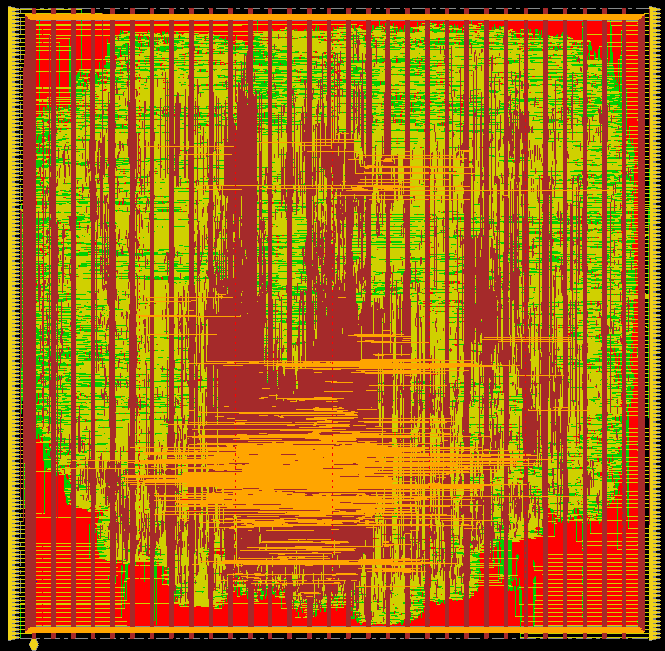
\includegraphics[width=0.45\textwidth]{fig_layout_v2_d256.png}\hspace{0.04\textwidth}
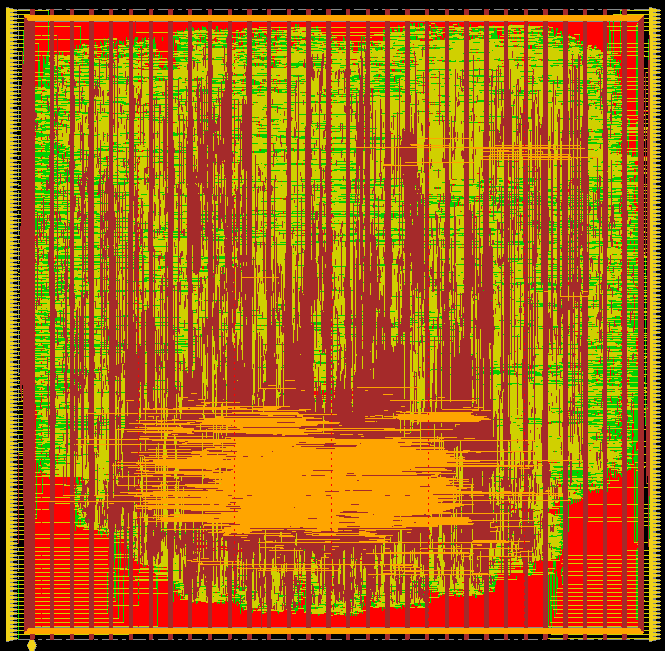
\includegraphics[width=0.45\textwidth]{fig_layout_v3_d256.png}\\[2pt]
\small (a) v2 \hspace{0.4\textwidth} (b) v3
\caption{Routed layouts at depth \R{sz.256} (merge-off netlists), \R{p15.met} ns clock after the two hold passes,
meeting setup and hold at the typical corner; same scale. Core area \R{p15.core.v2}\,\umsq{} (v2) and
\R{p15.core.v3}\,\umsq{} (v3) (P15)}
\label{fig:layout}
\end{figure}

Gate-level simulation and power after routing were run on the \R{p15.gls.period} ns layouts, which meet setup and hold
at the typical corner, with the routed netlist, its SDF and its extracted parasitics (Table~\ref{tab:p15pow}). v3 needs
\R{p15.dE.row1M.abs} to \R{p15.dE.row0.abs}\% less energy per request than v2, again because it needs fewer cycles.
Registers and the clock tree take all but \R{p15.logic.lo} to \R{p15.logic.hi}\% of the power: holding every line in
flip-flops dominates the power, which makes clock gating or SRAM storage the next step to try. These figures are not
comparable with Table~\ref{tab:p13}, which has no clock tree and no parasitics.

\begin{table}[ht]
\centering
\caption{Post-route power and energy, depth-\R{sz.256} layouts at \R{p15.gls.period} ns, mode 0, typical corner, path delays
annotated (P15)}
\label{tab:p15pow}
\begin{tabular}{@{}llccccc@{}}
\toprule
Version & Slice & Power (mW) & Energy (pJ/request) & Registers (\%) & Clock tree (\%) & Logic (\%) \\
\midrule
v2 & row0 & \R{p15.mW.v2.row0} & \R{p15.E.v2.row0} & \R{p15.reg.v2.row0} & \R{p15.clk.v2.row0} & \R{p15.logic.v2.row0} \\
v2 & row1M & \R{p15.mW.v2.row1M} & \R{p15.E.v2.row1M} & \R{p15.reg.v2.row1M} & \R{p15.clk.v2.row1M} & \R{p15.logic.v2.row1M} \\
v3 & row0 & \R{p15.mW.v3.row0} & \R{p15.E.v3.row0} & \R{p15.reg.v3.row0} & \R{p15.clk.v3.row0} & \R{p15.logic.v3.row0} \\
v3 & row1M & \R{p15.mW.v3.row1M} & \R{p15.E.v3.row1M} & \R{p15.reg.v3.row1M} & \R{p15.clk.v3.row1M} & \R{p15.logic.v3.row1M} \\
\bottomrule
\end{tabular}
\end{table}

\section{Corners and the I/O hold explanation}
The layouts were optimised at the typical corner only, so failures at other corners are expected; P16 re-timed the
existing layouts at a slow and a fast corner without changing them (Table~\ref{tab:p16}). Typical-corner re-timing reproduces the place-and-route reports; setup fails at the slow corner for every design and is
met at the fast corner. The derived slow-corner period, the place-and-route period minus the slow-corner setup
WNS of the same layout, is \R{p16.dp.v2.10} ns for v2 and \R{p16.dp.v3.10} ns for v3 at \R{p15.met} ns; it ignores hold
and is not a measurement. Here v3 is ahead, the opposite sign to the typical-corner difference at \R{p15.fail} ns, which
suggests that both differences lie within the variation of the flow.

\begin{table}[ht]
\centering
\caption{Worst setup / hold slack (ns) of the routed designs per corner, no re-optimisation (P16)}
\label{tab:p16}
\begin{tabular}{@{}lcccc@{}}
\toprule
Design & Period (ns) & Typical & Slow & Fast \\
\midrule
v3, depth \R{sz.16} & \R{p15.d16.period} & \R{p16t.d16v3.08.tt.s} / \R{p16t.d16v3.08.tt.h} & \R{p16t.d16v3.08.ss.s} / \R{p16t.d16v3.08.ss.h} & \R{p16t.d16v3.08.ff.s} / \R{p16t.d16v3.08.ff.h} \\
v2, depth \R{sz.256} & \R{p15.met} & \R{p16t.d256v2.10.tt.s} / \R{p16t.d256v2.10.tt.h} & \R{p16t.d256v2.10.ss.s} / \R{p16t.d256v2.10.ss.h} & \R{p16t.d256v2.10.ff.s} / \R{p16t.d256v2.10.ff.h} \\
v3, depth \R{sz.256} & \R{p15.met} & \R{p16t.d256v3.10.tt.s} / \R{p16t.d256v3.10.tt.h} & \R{p16t.d256v3.10.ss.s} / \R{p16t.d256v3.10.ss.h} & \R{p16t.d256v3.10.ff.s} / \R{p16t.d256v3.10.ff.h} \\
v2, depth \R{sz.256} & \R{p15.gls.period} & \R{p16t.d256v2.11.tt.s} / \R{p16t.d256v2.11.tt.h} & \R{p16t.d256v2.11.ss.s} / \R{p16t.d256v2.11.ss.h} & \R{p16t.d256v2.11.ff.s} / \R{p16t.d256v2.11.ff.h} \\
v3, depth \R{sz.256} & \R{p15.gls.period} & \R{p16t.d256v3.11.tt.s} / \R{p16t.d256v3.11.tt.h} & \R{p16t.d256v3.11.ss.s} / \R{p16t.d256v3.11.ss.h} & \R{p16t.d256v3.11.ff.s} / \R{p16t.d256v3.11.ff.h} \\
\bottomrule
\end{tabular}
\end{table}

\enlargethispage{2\baselineskip}Hold fails at the slow corner for the depth-\R{sz.256} layouts in the I/O path group only, while register-to-register hold
is met. Path reports of the v3 \R{p15.met} ns layout explain this. The constraints give the inputs a delay of
\R{p16.io.indelay} ns on the ideal clock edge, but at the slow corner the capturing register's clock arrives at
\R{p16.io.clk} ns through the propagated clock tree, so the hold slack is \R{p16.io.slack} ns; of the failing paths,
all but \R{d.in2reg.other} start at an input, and no register-to-output path fails. At the typical corner the saved
database holds a clock source latency of \R{p16.io.lat} ns, written by the tool during the flow, which cancels the
\R{p16.io.tree} ns tree delay for these paths (slack \R{p16.io.ttslack} ns); the added corners have none. At the fast
corner hold fails in the I/O group and, in the \R{p15.met} ns layouts, on some register-to-register paths. Sign-off would need per-corner I/O constraints or multi-corner optimisation; neither was done.

\chapter{Engineering and Reproducibility Practices}\label{ch:practice}
\section{Numbers from files}
No number may appear without a results file behind it, and no number is estimated or rounded up. Most phases write their tables with a script that reads the tool outputs, and \path{tools/make_tables.py} builds \path{results/P7/TABLES.md} from committed files only, reading them
with \texttt{git show HEAD:<path>} so that an uncommitted file cannot feed a table. The paper and this report go one
step further: every number is a macro generated by \path{tools/make_paper_macros.py}, which extracts it from a
results file by table row and column or by a regular expression and writes the source next to the definition, and
\path{tools/paper_numbers_check.py} fails the build on any digit typed directly into the text, a table or a caption.
Hit rates are rounded half-up to two decimals with the full value kept in the comment; differences, ratios and unit conversions are computed by the generator from the full values, with the formula recorded next to the definition; every other value appears as written in the file. 

\section{Confidentiality of the licensed library}
The commercial library is used under a licence, and the repository is public. The library, its documentation and its
technology files never leave the laboratory server and are never opened; only file names and the reports of the project's own runs are used. Raw reports, logs, netlists and SDF files stay off the repository; only aggregate tables and summaries
are committed, with Prof.\ Mane's approval. No library name, cell name, file name, path, server address or user name
may appear in a tracked file. Before every commit \path{tools/check_no_lib_leak.py} scans all tracked files against
generic patterns and against identifying patterns kept in a local file that is itself never committed, and reports only file, line and pattern number. The layout screenshots used in
Fig.~\ref{fig:layout} were cropped to the layout canvas because their window title showed a user name and the side
panel showed layer names; the originals are never committed. The paper names the vendor and node with Prof.\ Mane's approval, this report uses the same wording, and nothing else from the kit is named.

\section{Cluster workflow}
All heavy work on Sharanga runs as batch jobs: CPU trace simulations on the compute partition and GPU jobs on the H100 and H200 partitions, chained with job dependencies instead of polling. Each cluster phase uses driver or job scripts, records its job identifiers, copies its results back to the repository and commits them, because the scratch file system may be
purged.

\section{The scratch purge and the environment rebuild}
During P14, between its preparation and its main jobs, the scratch file system was purged and part of the Python environment disappeared; the next GPU jobs failed before profiling because files of the environment were missing. The environment was rebuilt offline from a
pinned list of the exact package builds (\path{cluster/dlrm_cache.explicit.txt}) with checksum-verified archives: the
rebuilt environment has \R{env.pkgs} packages and lists \R{env.files} files, with \R{env.missing} missing
(\path{results/P14/env_rebuild/}). Since then the job scripts that use the environment start with an environment check and stop with a clear message if it fails, and the checksums of the data files are recorded in \path{results/P2/data_hashes.txt}.

\section{Long jobs on the laboratory server}
The laboratory server is reached only through one authenticated connection, and jobs started from a login session
end when the session closes; a test showed that \texttt{nohup} did not survive logout. With lingering enabled for the
user, long Genus, Xcelium and Innovus jobs now run as \texttt{systemd-run -{}-user} units with a unique name and
survive logout. At most four tool jobs run at a time.

\chapter{Corrections Made During the Semester}\label{ch:corr}
\section{Audit of earlier claims}
Phase P7 checked \R{p7.a.n} claims of the earlier manuscript and README against committed files: \R{p7.a.contra}
were contradicted by a file, \R{p7.a.unsup} had no results file, \R{p7.a.notrerun} were reproduced from older
evidence that was not re-run, and \R{p7.a.sup} was supported (\path{results/P7/CLAIMS.md}). It also stated
\R{p7.b.n} new claims with their evidence and limits, of which \R{p7.b.sup} are supported and \R{p7.b.notrerun} rest on
older evidence. The main corrections are listed in Table~\ref{tab:corr}; the earlier values are not repeated here.

\begin{table}[ht]
\centering
\caption{Main corrected claims of the earlier manuscript (\protect\path{results/P7/CLAIMS.md})}
\label{tab:corr}
\small
\begin{tabularx}{\textwidth}{@{}>{\raggedright\arraybackslash}p{0.3\textwidth}>{\raggedright\arraybackslash}p{0.16\textwidth}L@{}}
\toprule
Earlier claim & Status & Correction \\
\midrule
\withdrawn{Synthesis results on a TSMC 28nm process (area, power, critical path, Fmax, slack)} & Unsupported,
withdrawn & No source file exists and no power analysis had been run; the figures are withdrawn. A Yosys generic-gate rerun of the old configuration, without a library file (gate counts only), gives \R{p7.rerun.cells} cells and \R{p7.rerun.ff} flip-flops, which contradicts the cell counts of
that table. The project's real implementation results are those of Chapters~\ref{ch:open} and~\ref{ch:c2}. \\
Share of inference time in ``embedding stalls'' & Contradicted & The figure was a ratio of two annotated profiler
ranges, not a stall measurement; the embedding kernel share in that launch-bound run was \R{old.kshare}\% (older
evidence, not re-run). \\
The claimed ratio of miss latency to hit latency & Contradicted & Picoseconds were read as cycles; no file measures the miss latency. \\
``Persistent saturating counters'' in the RTL & Contradicted & No RTL keeps a per-address history; mode 0 resets on
install and mode 1 keeps the slot's count. \\
gem5 hit rates at small L2 sizes; ``phase transition'' & Unsupported & No statistics files exist for those runs; gem5 models a CPU with DDR4, not a GPU; the trace study shows LFU-reset with oldest-first ties beating LRU at every size tested. \\
Reset on eviction causes the small-cache penalty & Contradicted & In trace simulation LFU-reset with oldest-first ties beats LRU everywhere tested; persistent LFU in a small shared cache loses (Chapter~\ref{ch:policy}), and so does the controller's lowest-slot rule (Chapter~\ref{ch:rtl}). \\
One Zipf exponent for Criteo & Contradicted & At \R{lab.10M} rows the per-table fits range from \R{p3.zipf.lo} to \R{p3.zipf.hi} (\R{p3.zipf.n} tables fitted). \\
``Criteo Terabyte'' dataset & Contradicted & The data is the Criteo Display Advertising Challenge file. \\
Waveform shows the counter values of specific lines & Contradicted & One of the two values is on a different line than claimed, and the waveform's testbench checks nothing. \\
\bottomrule
\end{tabularx}
\end{table}

\section{Corrections within this semester's work}
Several findings of this semester corrected the semester's own earlier assumptions:
\begin{itemize}
\item \textbf{Flow noise (P5c to P5d).} A noise estimate from one pair of designs was too small; eight same-logic
designs showed that the open flow alone moves Fmax by up to \R{p5d.noise.64.1}\%, so several earlier design
comparisons are within noise.
\item \textbf{ABC timing (P5e).} The delay target reached ABC but could not bind when ABC's own estimate was above both targets, and ABC's timer was optimistic; the timing-driven flow replaced it.
\item \textbf{Clock-pin power (P8).} OpenSTA's state-probability weighting of the flip-flop clock-pin energy was
biased; the clock-pin term was recalculated from the activity file.
\item \textbf{RTL and simulator (P8 to P9).} The assumption that the RTL implements the simulated LFU-reset policy was
wrong; the RTL-exact model and the tie-break finding followed.
\item \textbf{GPU counters (P14).} A test job averaged a percentage metric with the wrong weight and produced a hit rate of \R{p14.bad.pct}\%; the metric was replaced by sector counts, and the test numbers were not used.
\item \textbf{Address copies (P12).} Genus merged the per-group address copies despite the RTL's request to keep them;
the merge-off runs measured their effect.
\item \textbf{Power-rail shorts (P15).} The first place-and-route flow left shorts at the double-height cells; the
fixed flow excludes multi-row cells.
\item \textbf{I/O hold (P16).} The slow-corner hold failures were traced to the I/O constraints, not to the design.
\item \textbf{Paper.} Independent reviews of the paper draft narrowed overstated claims and added missing conditions, and a typing error in the status file was corrected.
\end{itemize}

\chapter{Limitations, Conclusions and Next Semester}\label{ch:concl}
\section{Limitations}
\begin{itemize}
\item \emph{Corners and runs.} All layouts were optimised at the typical corner only, and every design point is one
run; the bracket depends on the flow settings (other settings failed at periods up to \R{p15.oldfail} ns).
\item \emph{Timing in simulation.} The SDF simulations annotate no timing checks, so setup and hold rest on static
timing analysis at the typical corner.
\item \emph{Energy.} Activity is simulated for \R{p15.cov.v2} to \R{p15.cov.v3}\% of the driver nets after routing;
cycles per miss come from the testbench's fill handshake, a random delay of up to \R{p13.fill.max} cycles, not from a
memory system; the two slices come from one dataset.
\item \emph{Scope.} One dataset (the first \R{lab.10M} of \R{ds.rows} rows) and one within-row access order; hardware
built up to \R{sz.256} entries, larger sizes simulated with the RTL-exact model; each line holds a data word, not a
full vector.
\item \emph{Frequency.} The pre-layout runs meet \R{p12.br.256.met} ns at depth \R{sz.256} and the routed layouts
\R{p15.met} ns, probably because the pre-layout runs have no wire load, parasitics or clock tree; these effects were
not separated.
\item \emph{GPU.} Counters were measured on one H100 only, with one vector size and one lookup per bag.
\end{itemize}

\section{Conclusions}
Frequency-based replacement helps embedding caches on Criteo, but how counts are kept matters, and in a shared cache
history-keeping LFU loses to LRU at small sizes. In this controller, on Criteo, in one shared cache of \R{sz.256} to \R{sz.100000} entries, the tie-break of the victim search decides whether the cache beats LRU: with lowest-index ties a new line that starts at count one becomes the next victim unless it is hit first, and the exact model of the controller loses to LRU at every size simulated in that range. A single pointer register (Rotate-victim) restores oldest-first LFU, and in a 28nm FD-SOI flow
through place and route the fix keeps the clock period of the original design at the typical corner and lowers energy
per request by \R{p15.dE.row1M.abs} to \R{p15.dE.row0.abs}\% in post-route simulation with a testbench fill model.
Equally important for the project, every number is now traceable to a file, and the earlier unsupported claims have
been withdrawn.

\section{Work planned for the next semester}
The plan (\path{docs/plan_next_sem/plan.pdf}) ranks eight goals, each with a measurable success criterion, on a
fourteen-week timeline that puts the laboratory-server work early, in blocks of at most four tool jobs:
\begin{enumerate}[label=\alph*.]
\item multi-corner sign-off with block-level I/O constraints and multi-mode multi-corner optimisation over the
typical, slow and fast corners, with met periods per corner for v2 and v3;
\item clock gating and, if the design kit provides SRAM macros, SRAM storage for the data array, with power and energy
per request before and after in the same flow;
\item a set-associative controller with Rotate-victim per set, so that caches of a thousand to a hundred thousand entries exist in RTL and the smallest in layout;
\item a cycle-level DRAM model behind the cache instead of the testbench fill model, and energy per request
recomputed with it;
\item a second dataset and a second access order for the tie-break study;
\item repeated place and route with varied utilisation and seeds to bound the v2/v3 timing difference;
\item SDF timing-check annotation, and H200 counters once the administrators grant access;
\item the paper: Prof.\ Mane's comments, submission and revision.\enlargethispage{2\baselineskip}
\end{enumerate}


\appendix
\chapter{Phase Summary}\label{app:phases}
\begin{small}
\setlength{\tabcolsep}{4pt}
\begin{longtable}{@{}>{\raggedright\arraybackslash}p{0.08\textwidth}>{\raggedright\arraybackslash}p{0.2\textwidth}>{\raggedright\arraybackslash}p{0.2\textwidth}>{\raggedright\arraybackslash}p{0.31\textwidth}>{\raggedright\arraybackslash}p{0.12\textwidth}@{}}
\caption{Phases of the semester: question, method, key result and results folder}\label{tab:phases}\\
\toprule
Phase & Question & Method & Key result & Folder \\
\midrule
\endfirsthead
\toprule
Phase & Question & Method & Key result & Folder \\
\midrule
\endhead
P0 & What does the cluster offer? & Partition, storage and module survey & H100 and H200 partitions found; scratch
work directory created & \path{results/P0} \\
P1 & Can the counter scheme be selected? & \texttt{COUNTER\_MODE} parameter, tests, mutation & Mode 0 and mode 1 pass
\R{rtl.tests} tests; mutation \R{p1.runs} runs, all non-equivalent killed & \path{results/P1} \\
P2 & Is the dataset intact? & Download with checksum, line checks & \R{ds.rows} rows, every categorical field a hash or
empty & \path{results/P2} \\
P3 & Does LFU beat LRU per table? & Trace simulation, seven policies & Both LFU variants beat LRU at every capacity;
\R{p3.10M.256.LFUr}\% against \R{p3.10M.256.LRU}\% at \R{sz.256} vectors (\R{lab.10M}) & \path{results/P3} \\
P3b & And in one shared cache? & Shared-cache simulator & LFU-reset \R{p3b.10M.256.LFUr}\%, LRU \R{p3b.10M.256.LRU}\%,
LFU-persistent \R{p3b.10M.256.LFUp}\% at \R{sz.256} entries (\R{lab.10M}) & \path{results/P3b} \\
P4 & How long do embedding lookups take on GPUs? & CUDA-event timing, H100 and H200 & Embedding share
\R{p4.b8k.h100.lo} to \R{p4.b8k.h100.hi} at batch \R{p4.b.max} (H100); small batches launch-bound &
\path{results/P4} \\
P5 & How fast is the RTL on an open library? & Yosys, NanGate45, OpenSTA & Baseline \R{p5.f.256}\,MHz at depth
\R{sz.256}, pre-layout & \path{results/P5} \\
P5b to P5d & Can restructuring help? & Reduction and priority trees & \R{p5d.f.256}\,MHz at depth \R{sz.256}; flow noise
up to \R{p5d.noise.64.1}\% & \path{results/P5b} to \path{P5d} \\
P5e & Is the synthesis flow sound? & Timing-driven ABC flow & \R{p5e.f.256}\,MHz at depth \R{sz.256}, above the noise
band & \path{results/P5e} \\
P5f & Do the netlists match the RTL? & Zero-delay GLS, equivalence & \R{p5f.netlists} netlists, \R{p5f.mism}
mismatching cycles; depth-\R{sz.16} equivalence proven & \path{results/P5f_gls} \\
P7 & Which earlier claims hold? & Claims audit, tables from files & \R{p7.a.contra} contradicted, \R{p7.a.unsup}
unsupported of \R{p7.a.n} & \path{results/P7} \\
P8 & Where does the power go? & OpenSTA power from GLS activity & Flip-flop clock pins dominate; OpenSTA weighting biased (\R{p8.bias}\% in one test) & \path{results/P8} \\
P9 & Why do RTL and simulator differ? & RTL-exact model, ablation & Lowest-slot tie-break: v2 rule below LRU from
\R{sz.256} to \R{sz.100000} entries & \path{results/P9} \\
P10 & Does the fix work in RTL? & Rotate-victim in \texttt{rtl/v3}, lockstep & \R{p10.mism} mismatches in
\R{p10.runs} runs & \path{results/P10} \\
P11 & Full traces, synthesis and GLS of v3 & Simulation, open flow, GLS & v3 equals LFU-reset at \R{sz.16} to
\R{sz.256} entries; Fmax change within noise & \path{results/P11} \\
P12 & 28nm synthesis & Genus brackets, merge-off & \R{p12.br.256.met} met, \R{p12.br.256.fail} ns failed at depth
\R{sz.256}; merge-off \R{p12.mo.v2}\% / \R{p12.mo.v3}\% Fmax & \path{results/P12} \\
P13 & 28nm GLS and energy & Xcelium lockstep, Genus power & v3 \R{p13.dE.row1M.abs} to \R{p13.dE.row0.abs}\% less
energy per request, pre-layout & \path{results/P13} \\
P14 & GPU L2 behaviour & Nsight Compute on one H100 & L2 read hit \R{p14.pt.64}\% to \R{p14.pt.16384}\% as the batch
grows & \path{results/P14} \\
P15 & Place and route & Innovus, post-route GLS and power & Both meet \R{p15.met}, fail \R{p15.fail} ns; v3
\R{p15.dE.row1M.abs} to \R{p15.dE.row0.abs}\% less energy & \path{results/P15} \\
P16 & Other corners & Re-timing at slow and fast corners & Derived slow-corner periods \R{p16.dp.v2.10} and
\R{p16.dp.v3.10} ns; I/O hold explained & \path{results/P16} \\
\bottomrule
\end{longtable}
\end{small}

\chapter{Repository Tags and Milestone Commits}\label{app:commits}
The repository is at \url{https://github.com/idealxdxrsh/Cache-Policy-Phase-Transition-in-DLRM-Workloads}. The tag
\texttt{rtl-v2-baseline} (\texttt{0d66a3a}) marks the first synthesised RTL, \texttt{rtl-v2-final}
(\texttt{7705a7b}) the final v2 controller, and the branch \texttt{rtl-v3} holds v3 and all later work.

\begin{small}
\begin{longtable}{@{}>{\raggedright\arraybackslash}p{0.3\textwidth}>{\raggedright\arraybackslash}p{0.65\textwidth}@{}}
\caption{Milestone commits}\label{tab:commits}\\
\toprule
Commit & Milestone \\
\midrule
\endfirsthead
\toprule
Commit & Milestone \\
\midrule
\endhead
\texttt{379a5ce} & P0: cluster set-up check \\
\texttt{10cd602} & P1: \texttt{COUNTER\_MODE}, per-mode tests, mutation script \\
\texttt{22935f6} & P2: Criteo data downloaded and verified \\
\texttt{b167b20} & P3: per-table trace simulation results \\
\texttt{35c1d7d}, \texttt{cc9e875} & P3b: shared-cache results at the two trace lengths \\
\texttt{04c34be} & P4: GPU timing results \\
\texttt{b5d85b7} & P5: NanGate45 baseline synthesis \\
\texttt{4debe84}, \texttt{73016e0}, \texttt{7705a7b} & P5b, P5c, P5d: tree restructuring; final v2 RTL \\
\texttt{b69a931} & P5e: timing-driven flow \\
\texttt{4188580}, \texttt{42a8201}, \texttt{02518be} & P5f: gate-level simulation, equivalence, cluster lockstep \\
\texttt{1575c09}, \texttt{e615881} & P7: claims audit and tables from committed files \\
\texttt{5d51bad} & P7: first rewrite of the paper from the audited tables \\
\texttt{7493a68}, \texttt{8c2bc9f} & P8: open-flow power analysis \\
\texttt{03d314d}, \texttt{7dd5f5c} & P9: RTL-exact model and full-trace results \\
\texttt{25ff5d5} & P10: Rotate-victim in \texttt{rtl/v3} \\
\texttt{aacfe16}, \texttt{d8a74c6}, \texttt{6316b02} & P11: v3 synthesis, full traces and GLS \\
\texttt{1a9a928}, \texttt{ccb3650} & P12, P13: commercial synthesis, GLS and power; aggregate publication \\
\texttt{6b2863e} & P14: H100 counters on the Criteo stream \\
\texttt{f1f7e6a} & Environment rebuild after the scratch purge \\
\texttt{c963e4e}, \texttt{7ededd6}, \texttt{0335af2}, \texttt{7f3aa5c} & P15: place and route, short fix, post-route
GLS and power, final brackets \\
\texttt{30438da}, \texttt{ab20c1d} & P16: corners and the I/O hold diagnosis \\
\texttt{854f8df}, \texttt{d5ddcfe} & Paper rewrite and revision \\
\texttt{c09c0a7} & Plan for the next semester \\
\bottomrule
\end{longtable}
\end{small}

\bibliographystyle{IEEEtran}
\bibliography{../../paper/v2/refs}

\end{document}
